%%%%%%%%%%%%%%%%%%%%%%%%%%%%% Thesis.tex %%%%%%%%%%%%%%%%%%%%%%%%%%%%%%%
%                                                                      %
%  ---------- Master of Science Dissertation template ----------       %
%                                                                      %
%  Template for the Master Thesis according to the regulations         %
%  published by the Academic Board (Direcção Académica) at IST.        %
%                                                                      %
%  For up-to-date guide, please refer to the official website          %
%
% https://tecnico.ulisboa.pt/pt/ensino/estudar-no-tecnico/informacoes-academicas/dissertacao-de-mestrado/
%                                                                      %
%       Andre C. Marta                                                 %
%       Area Cientifica de Mecanica Aplicada e Aeroespacial            %
%       Departamento de Engenharia Mecanica                            %
%       Instituto Superior Tecnico                                     %
%       Av. Rovisco Pais                                               %
%       1049-001 Lisboa                                                %
%       Portugal                                                       %
%       Tel: +351 21 841 9469                                          %
%                        3469 (extension)                              %
%       Email: andre.marta@tecnico.ulisboa.pt                          %
%                                                                      %
%  Created:       Jan 20, 2011                                         %
%  Last Modified: JUn 29, 2022                                         %
%                                                                      %
%%%%%%%%%%%%%%%%%%%%%%%%%%%%%%%%%%%%%%%%%%%%%%%%%%%%%%%%%%%%%%%%%%%%%%%%
%  Revision history                                                    %
%  v1 - 2011/01/24 - original template                                 %
%  v2 - 2012/10/30 - new IST image and glossary support                %
%  v3 - 2013/12/10 - update according to 2012/13 official guide        %
%  v4 - 2014/02/28 - new default for bibliography style                %
%  v5 - 2014/05/07 - update according to 2013/14 official guide        %
%  v6 - 2015/07/02 - cover page format fixed,                          %
%                    contents page numbering fixed,                    %
%                    better language support,                          %
%                    enhanced examples of tables,                      %
%                    new option for appendix page numbering format,    %
%                    custom bibliography style                         %
%  v7 - 2018/02/19 - multiple citations compressed                     %
%  v8 - 2019/05/13 - added examples (pseudo-code)                      %
%  v9 - 2020/03/03 - added French language support                     %
%                    indented first paragraphs                         %
%  v10- 2021/01/29 - place caption above table                         %
%  v11- 2022/06/29 - included Declaration of original work             %
%%%%%%%%%%%%%%%%%%%%%%%%%%%%%%%%%%%%%%%%%%%%%%%%%%%%%%%%%%%%%%%%%%%%%%%%
%                                                                      %
% To generate the PDF file, type "make" at the terminal prompt.        %
%                                                                      %
% The IST template LaTeX package was created by the author             %
% and it can be downloaded from:                                       %
% https://fenix.ist.utl.pt/homepage/ist31052/                          %
%                                                                      %
% The external packages can be downloaded from                         %
% the Comprehensive TeX Archive Network at http://www.ctan.org/        %
%                                                                      %
% List of LaTex symbols:                                               %
% http://www.ctan.org/tex-archive/info/symbols/comprehensive/          %
%                                                                      %
% Help with LaTex can be found at                                      %
% http://www.giss.nasa.gov/tools/latex/ltx-2.html                      %
% http://en.wikibooks.org/wiki/LaTeX                                   %
%%%%%%%%%%%%%%%%%%%%%%%%%%%%%%%%%%%%%%%%%%%%%%%%%%%%%%%%%%%%%%%%%%%%%%%%

%%%%%%%%%%%%%%%%%%%%%%%%%%%%%%%%%%%%%%%%%%%%%%%%%%%%%%%%%%%%%%%%%%%%%%%%
%     Preamble                                                         %
%%%%%%%%%%%%%%%%%%%%%%%%%%%%%%%%%%%%%%%%%%%%%%%%%%%%%%%%%%%%%%%%%%%%%%%%



% ----------------------------------------------------------------------
%  Set the document class
% ----------------------------------------------------------------------
\documentclass[10pt,a4paper,twoside]{report}

\usepackage[portuguese]{babel}
\usepackage{array}
\usepackage{multirow}
\usepackage[utf8]{inputenc}
\usepackage[toc]{glossaries}
\usepackage{amsmath}
\usepackage[table]{xcolor}



\definecolor{orange}{rgb}{1,0.647,0}
\definecolor{grayblue}{rgb}{0.5, 0.5, 1}
\makeglossaries


% ----------------------------------------------------------------------
% Define external packages, language, margins, fonts and new commands
% ----------------------------------------------------------------------
%%%%%%%%%%%%%%%%%%%%%%%%%%%%%%%%%%%%%%%%%%%%%%%%%%%%%%%%%%%%%%%%%%%%%%%%
%                                                                      %
%     File: Thesis_Preamble.tex                                        %
%     Tex Master: Thesis.tex                                           %
%                                                                      %
%     Author: Andre C. Marta                                           %
%     Last modified : 29 Jun 2022                                      %
%                                                                      %
%%%%%%%%%%%%%%%%%%%%%%%%%%%%%%%%%%%%%%%%%%%%%%%%%%%%%%%%%%%%%%%%%%%%%%%%

% 'natbib' package
%
% Flexible bibliography support.
% http://www.ctan.org/tex-archive/macros/latex/contrib/natbib/
%
% > produce author-year style citations
%
% \citet  and \citep  for textual and parenthetical citations, respectively
% \citet* and \citep* that print the full author list, and not just the abbreviated one
% \citealt is the same as \citet but without parentheses. Similarly, \citealp is \citep without parentheses
% \citeauthor
% \citeyear
% \citeyearpar
%
%% natbib options can be provided when package is loaded \usepackage[options]{natbib}
%%
%% Following options are valid:
%%
%%   round  -  round parentheses are used (default)
%%   square -  square brackets are used   [option]
%%   curly  -  curly braces are used      {option}
%%   angle  -  angle brackets are used    <option>
%%   semicolon  -  multiple citations separated by semi-colon (default)
%%   colon  - same as semicolon, an earlier confusion
%%   comma  -  separated by comma
%%   authoryear - for author–year citations (default)
%%   numbers-  selects numerical citations
%%   super  -  numerical citations as superscripts, as in Nature
%%   sort   -  sorts multiple citations according to order in ref. list
%%   sort&compress   -  like sort, but also compresses numerical citations
%%   compress - compresses without sorting
%%
% ******************************* SELECT *******************************
%\usepackage{natbib}          % <<<<< References in alphabetical list Correia, Silva, ...
\usepackage[numbers,sort&compress]{natbib} % <<<<< References in numbered list [1],[2],...
% ******************************* SELECT *******************************


% 'notoccite' package
%
% Prevent trouble from citations in table of contents, etc.
% http://ctan.org/pkg/notoccite
%
% > If you have \cite com­mands in \sec­tion-like com­mands, or in \cap­tion,
%   the ci­ta­tion will also ap­pear in the ta­ble of con­tents, or list of what­ever.
%   If you are also us­ing an un­srt-like bib­li­og­ra­phy style, these ci­ta­tions will
%   come at the very start of the bib­li­og­ra­phy, which is con­fus­ing. This pack­age
%   sup­presses the ef­fect.
%
\usepackage{notoccite}


% ----------------------------------------------------------------------
% Define document language.
% ----------------------------------------------------------------------

% 'inputenc' package
%
% Accept different input encodings.
% http://www.ctan.org/tex-archive/macros/latex/base/
%
% > allows typing non-english text in LaTeX sources.
%
% ******************************* SELECT *******************************
%\usepackage[latin1]{inputenc} % <<<<< Windows
\usepackage[utf8]{inputenc}   % <<<<< Linux
% ******************************* SELECT *******************************


% 'babel' package
%
% Multilingual support for Plain TeX or LaTeX.
% http://www.ctan.org/tex-archive/macros/latex/required/babel/
%
% > sets the variable names according to the language selected
%
% ******************************* SELECT *******************************
%\usepackage[portuguese]{babel} % <<<<< Portuguese
\usepackage[english]{babel} % <<<<< English
%\usepackage[francais]{babel} % <<<<< French (requires package texlive-lang-french)
% ******************************* SELECT *******************************


% List of LaTeX variable names: \abstractname, \appendixname, \bibname,
%   \chaptername, \contentsname, \listfigurename, \listtablename, ...)
% http://www.tex.ac.uk/cgi-bin/texfaq2html?label=fixnam
%
% Changing the words babel uses (uncomment and redefine as necessary...)
%
\newcommand{\acknowledgments}{@undefined} % new LaTeX variable name
%
% > English
%
\addto\captionsenglish{\renewcommand{\acknowledgments}{Acknowledgments}}
%\addto\captionsenglish{\renewcommand{\contentsname}{Contents}}
%\addto\captionsenglish{\renewcommand{\listtablename}{List of Tables}}
%\addto\captionsenglish{\renewcommand{\listfigurename}{List of Figures}}
%\addto\captionsenglish{\renewcommand{\nomname}{Nomenclature}}
%\addto\captionsenglish{\renewcommand{\glossaryname}{Glossary}}
%\addto\captionsenglish{\renewcommand{\acronymname}{List of Acronyms}}
%\addto\captionsenglish{\renewcommand{\bibname}{References}} % Bibliography
%\addto\captionsenglish{\renewcommand{\appendixname}{Appendix}}

% > French
%
\addto\captionsfrench{\renewcommand{\acknowledgments}{Remerciements}}
%\addto\captionsfrench{\renewcommand{\contentsname}{Table des matières}}
%\addto\captionsfrench{\renewcommand{\listtablename}{Liste des tableaux}}
\addto\captionsfrench{\renewcommand{\listfigurename}{Liste des figures}} % Table des figures
%\addto\captionsfrench{\renewcommand{\nomname}{Nomenclature}}
%\addto\captionsfrench{\renewcommand{\glossaryname}{Glossaire}}
%\addto\captionsfrench{\renewcommand{\acronymname}{Liste des acronymes}}
%\addto\captionsfrench{\renewcommand{\bibname}{Bibliographie}}
%\addto\captionsfrench{\renewcommand{\appendixname}{Annexe}}

% > Portuguese
%
\addto\captionsportuguese{\renewcommand{\acknowledgments}{Agradecimentos}}
%\addto\captionsportuguese{\renewcommand{\contentsname}{Conte\'{u}do}}
%\addto\captionsportuguese{\renewcommand{\listtablename}{Lista de Figuras}}
%\addto\captionsportuguese{\renewcommand{\listfigurename}{Lista de Tabelas}}
\addto\captionsportuguese{\renewcommand{\nomname}{Lista de S\'{i}mbolos}} % Nomenclatura
%\addto\captionsportuguese{\renewcommand{\glossary}{Gloss\'{a}rio}}
%\addto\captionsportuguese{\renewcommand{\acronymname}{Lista de Abrevia\c{c}\~{o}es}}
%\addto\captionsportuguese{\renewcommand{\bibname}{Refer\^{e}ncias}} % Bibliografia
%\addto\captionsportuguese{\renewcommand{\appendixname}{Anexo}} % Apendice


% ----------------------------------------------------------------------
% Define cover fields in both english and portuguese.
% ----------------------------------------------------------------------
%
\newcommand{\coverThesis}{@undefined} % new LaTeX variable name
\newcommand{\coverSupervisors}{@undefined} % new LaTeX variable name
\newcommand{\coverExaminationCommittee}{@undefined} % new LaTeX variable name
\newcommand{\coverChairperson}{@undefined} % new LaTeX variable name
\newcommand{\coverSupervisor}{@undefined} % new LaTeX variable name
\newcommand{\coverMemberCommittee}{@undefined} % new LaTeX variable name
% > English
\addto\captionsenglish{\renewcommand{\coverThesis}{Thesis to obtain the Master of Science Degree in}}
\addto\captionsenglish{\renewcommand{\coverSupervisors}{Supervisor(s)}}
\addto\captionsenglish{\renewcommand{\coverExaminationCommittee}{Examination Committee}}
\addto\captionsenglish{\renewcommand{\coverChairperson}{Chairperson}}
\addto\captionsenglish{\renewcommand{\coverSupervisor}{Supervisor}}
\addto\captionsenglish{\renewcommand{\coverMemberCommittee}{Member of the Committee}}
% > French
\addto\captionsfrench{\renewcommand{\coverThesis}{Th\`ese pour l'obtention du Maîtrise des Sciences en}}
\addto\captionsfrench{\renewcommand{\coverSupervisors}{Directeur(s) de th\`ese}}
\addto\captionsfrench{\renewcommand{\coverExaminationCommittee}{Jury}}
\addto\captionsfrench{\renewcommand{\coverChairperson}{Pr\'esident}}
\addto\captionsfrench{\renewcommand{\coverSupervisor}{Directeur de th\`ese}}
\addto\captionsfrench{\renewcommand{\coverMemberCommittee}{Rapporteur}}
% > Portuguese
\addto\captionsportuguese{\renewcommand{\coverThesis}{Projeto Integrador de 2º ciclo em}}
\addto\captionsportuguese{\renewcommand{\coverSupervisors}{Orientador(es)}}
\addto\captionsportuguese{\renewcommand{\coverExaminationCommittee}{J\'{u}ri}}
\addto\captionsportuguese{\renewcommand{\coverChairperson}{Presidente}}
\addto\captionsportuguese{\renewcommand{\coverSupervisor}{Orientador}}
\addto\captionsportuguese{\renewcommand{\coverMemberCommittee}{Vogal}}


% ----------------------------------------------------------------------
% Define Declaration of original work in both english and portuguese.
% ----------------------------------------------------------------------
%
\newcommand{\declarationTitle}{@undefined} % new LaTeX variable name
\newcommand{\declarationText}{@undefined}  % new LaTeX variable name
% > English
\addto\captionsenglish{\renewcommand{\declarationTitle}{Declaration}}
\addto\captionsenglish{\renewcommand{\declarationText}{I declare that this document is an original work of my own authorship and that it fulfills all the requirements of the Code of Conduct and Good Practices of the Universidade de Lisboa.}}
% > Portuguese
\addto\captionsportuguese{\renewcommand{\declarationTitle}{Declara\c{c}\~{a}o}}
\addto\captionsportuguese{\renewcommand{\declarationText}{Declaro que o presente documento \'{e} um trabalho original da minha autoria e que cumpre todos os requisitos do C\'{o}digo de Conduta e Boas Pr\'{a}ticas da Universidade de Lisboa.}}


% ----------------------------------------------------------------------
% Define default and cover page fonts.
% ----------------------------------------------------------------------

% Use Arial font as default
%
\renewcommand{\rmdefault}{phv}
\renewcommand{\sfdefault}{phv}

% Define cover page fonts
%
%         encoding     family       series      shape
%  \usefont{T1}     {phv}=helvetica  {b}=bold    {n}=normal
%                   {ptm}=times      {m}=normal  {sl}=slanted
%                                                {it}=italic
% see more examples at
% https://www.overleaf.com/learn/latex/Font_typefaces
% https://tug.org/FontCatalogue/
%
\def\FontLn{% 16 pt normal
  \usefont{T1}{phv}{m}{n}\fontsize{16pt}{16pt}\selectfont}
\def\FontLb{% 16 pt bold
  \usefont{T1}{phv}{b}{n}\fontsize{16pt}{16pt}\selectfont}
\def\FontMn{% 14 pt normal
  \usefont{T1}{phv}{m}{n}\fontsize{14pt}{14pt}\selectfont}
\def\FontMb{% 14 pt bold
  \usefont{T1}{phv}{b}{n}\fontsize{14pt}{14pt}\selectfont}
\def\FontSn{% 12 pt normal
  \usefont{T1}{phv}{m}{n}\fontsize{12pt}{12pt}\selectfont}


% ----------------------------------------------------------------------
% Define page margins and line spacing.
% ----------------------------------------------------------------------

% 'geometry' package
%
% Flexible and complete interface to document dimensions.
% http://www.ctan.org/tex-archive/macros/latex/contrib/geometry/
%
% > set the page margins (2.5cm minimum in every side, as per IST rules)
%
\usepackage{geometry}	
\geometry{verbose,tmargin=2.5cm,bmargin=2.5cm,lmargin=2.5cm,rmargin=2.5cm}

% 'setspace' package
%
% Set space between lines.
% http://www.ctan.org/tex-archive/macros/latex/contrib/setspace/
%
% > allow setting line spacing (line spacing of 1.5, as per IST rules)
%
\usepackage{setspace}
\renewcommand{\baselinestretch}{1.5}


% ----------------------------------------------------------------------
% Define paragraph formating.
% ----------------------------------------------------------------------

% 'indentfirst' package
%
% Indent first paragraph after section header.
% https://ctan.org/pkg/indentfirst
%
% > indent all paragraphs (as per IST rules)
%
\usepackage{indentfirst}	


% ----------------------------------------------------------------------
% Include external packages.
% Note that not all of these packages may be available on all system
% installations. If necessary, include the .sty files locally in
% the <jobname>.tex file directory.
% ----------------------------------------------------------------------

% 'graphicx' package
%
% Enhanced support for graphics.
% http://www.ctan.org/tex-archive/macros/latex/required/graphics/
%
% > extends arguments of the \includegraphics command
%
\usepackage{graphicx}


% 'color' package
%
% Colour control for LaTeX documents.
% http://www.ctan.org/tex-archive/macros/latex/required/graphics/
%
% > defines color macros: \color{<color name>}
%
%\usepackage{color}


% 'amsmath' package
%
% Mathematical enhancements for LaTeX.
% http://www.ctan.org/tex-archive/macros/latex/required/amslatex/
%
% > American Mathematical Society plain Tex macros
%
\usepackage{amsmath}  % AMS mathematical facilities for LaTeX.
\usepackage{amsthm}   % Typesetting theorems (AMS style).
\usepackage{amsfonts} % 


% 'wrapfig' package
%
% Produces figures which text can flow around.
% http://www.ctan.org/tex-archive/macros/latex/contrib/wrapfig/
%
% > wrap figures/tables in text (i.e., Di Vinci style)
%
% \usepackage{wrapfig}


% 'subfigure' package
%
% Deprecated: Figures divided into subfigures.
% http://www.ctan.org/tex-archive/obsolete/macros/latex/contrib/subfigure/
%
% > subcaptions for subfigures
%
\usepackage{subfigure}


% 'subfigmat' package
%
% Automates layout when using the subfigure package.
% http://www.ctan.org/tex-archive/macros/latex/contrib/subfigmat/
%
% > matrices of similar subfigures
%
\usepackage{subfigmat}


% 'url' package
%
% Verbatim with URL-sensitive line breaks.
% http://www.ctan.org/tex-archive/macros/latex/contrib/url/
%
% > URLs in BibTex
%
% \usepackage{url}


% 'varioref' package
%
% Intelligent page references.
% http://www.ctan.org/tex-archive/macros/latex/required/tools/
%
% > smart page, figure, table and equation referencing
%
%\usepackage{varioref}


% 'dcolumn' package
%
% Align on the decimal point of numbers in tabular columns.
% http://www.ctan.org/tex-archive/macros/latex/required/tools/
%
% > decimal-aligned tabular math columns
%
\usepackage{dcolumn}
\newcolumntype{d}{D{.}{.}{-1}} % column aligned by the point separator '.'
\newcolumntype{e}{D{E}{E}{-1}} % column aligned by the exponent 'E'


% 'verbatim' package
%
% Reimplementation of and extensions to LaTeX verbatim.
% http://www.ctan.org/tex-archive/macros/latex/required/tools/
%
% > provides the verbatim environment (\begin{verbatim},\end{verbatim})
%   and a comment environment (\begin{comment},  \end{comment})
%
% \usepackage{verbatim}


% 'moreverb' package
%
% Extended verbatim.
% http://www.ctan.org/tex-archive/macros/latex/contrib/moreverb/
%
% > supports tab expansion and line numbering
%
% \usepackage{moreverb}



% 'nomencl' package
%
% Produce lists of symbols as in nomenclature.
% http://www.ctan.org/tex-archive/macros/latex/contrib/nomencl/
%
% The nomencl package makes use of the MakeIndex program
% in order to produce the nomenclature list.
%
% Nomenclature
% 1) On running the file through LATEX, the command \makenomenclature
%    in the preamble instructs it to create/open the nomenclature file
%    <jobname>.nlo corresponding to the LATEX file <jobname>.tex and
%    writes the information from the \nomenclature commands to this file.
% 2) The next step is to invoke MakeIndex in order to produce the
%    <jobname>.nls file. This can be achieved by making use of the
%    command: makeindex <jobname>.nlo -s nomencl.ist -o <jobname>.nls
% 3) The last step is to invoke LATEX on the <jobname>.tex file once
%    more. There, the \printnomenclature in the document will input the
%    <jobname>.nls file and process it according to the given options.
%
% http://www-h.eng.cam.ac.uk/help/tpl/textprocessing/nomencl.pdf
%
% Nomenclature (produces *.nlo *.nls files)
\usepackage{nomencl}
\makenomenclature
%
% Group variables according to their symbol type
%
\RequirePackage{ifthen} 
\ifthenelse{\equal{\languagename}{english}}%
    { % English
    \renewcommand{\nomgroup}[1]{%
      \ifthenelse{\equal{#1}{R}}{%
        \item[\textbf{Roman symbols}]}{%
        \ifthenelse{\equal{#1}{G}}{%
          \item[\textbf{Greek symbols}]}{%
          \ifthenelse{\equal{#1}{S}}{%
            \item[\textbf{Subscripts}]}{%
            \ifthenelse{\equal{#1}{T}}{%
              \item[\textbf{Superscripts}]}{}}}}}%
    }{%
    \ifthenelse{\equal{\languagename}{french}}%
    { % French
    \renewcommand{\nomgroup}[1]{%
      \ifthenelse{\equal{#1}{R}}{%
        \item[\textbf{Symbole romains}]}{%
        \ifthenelse{\equal{#1}{G}}{%
          \item[\textbf{Symboles grecs}]}{%
          \ifthenelse{\equal{#1}{S}}{%
            \item[\textbf{Indices}]}{% lettre inférieure
            \ifthenelse{\equal{#1}{T}}{%
              \item[\textbf{Exposants}]}{}}}}}% lettre supérieure
    }{ % Portuguese
    \renewcommand{\nomgroup}[1]{%
      \ifthenelse{\equal{#1}{R}}{%
        \item[\textbf{Simbolos romanos}]}{%
        \ifthenelse{\equal{#1}{G}}{%
          \item[\textbf{Simbolos gregos}]}{%
          \ifthenelse{\equal{#1}{S}}{%
            \item[\textbf{Subscritos}]}{%
            \ifthenelse{\equal{#1}{T}}{%
              \item[\textbf{Sobrescritos}]}{}}}}}%
    }}%


% 'glossary' package
%
% Create a glossary.
% http://www.ctan.org/tex-archive/macros/latex/contrib/glossary/
%
% Glossary (produces *.glo *.ist files)
\usepackage[number=none]{glossary}
% (remove blank line between groups)
\setglossary{gloskip={}}
% (redefine glossary style file)
%\renewcommand{\istfilename}{myGlossaryStyle.ist}
\makeglossary


% 'rotating' package
%
% Rotation tools, including rotated full-page floats.
% http://www.ctan.org/tex-archive/macros/latex/contrib/rotating/
%
% > show wide figures and tables in landscape format:
%   use \begin{sidewaystable} and \begin{sidewaysfigure}
%   instead of 'table' and 'figure', respectively.
%
\usepackage{rotating}


% 'hyperref' package
%
% Extensive support for hypertext in LaTeX.
% http://www.ctan.org/tex-archive/macros/latex/contrib/hyperref/
%
% > Extends the functionality of all the LATEX cross-referencing
%   commands (including the table of contents, bibliographies etc) to
%   produce \special commands which a driver can turn into hypertext
%   links; Also provides new commands to allow the user to write adhoc
%   hypertext links, including those to external documents and URLs.
%
\usepackage[pdftex]{hyperref} % enhance documents that are to be
                              % output as HTML and PDF
\hypersetup{colorlinks,       % color text of links and anchors,
                              % eliminates borders around links
%            linkcolor=red,    % color for normal internal links
            linkcolor=black,  % color for normal internal links
            anchorcolor=black,% color for anchor text
%            citecolor=green,  % color for bibliographical citations
            citecolor=black,  % color for bibliographical citations
%            filecolor=magenta,% color for URLs which open local files
            filecolor=black,  % color for URLs which open local files
%            menucolor=red,    % color for Acrobat menu items
            menucolor=black,  % color for Acrobat menu items
%            pagecolor=red,    % color for links to other pages
            pagecolor=black,  % color for links to other pages
%            urlcolor=cyan,    % color for linked URLs
            urlcolor=black,   % color for linked URLs
	          bookmarks=true,         % create PDF bookmarks
	          bookmarksopen=false,    % don't expand bookmarks
	          bookmarksnumbered=true, % number bookmarks
	          pdftitle={Thesis},
            pdfauthor={Andre C. Marta},
            pdfsubject={Thesis Title},
            pdfkeywords={Thesis Keywords},
            pdfstartview=FitV,
            pdfdisplaydoctitle=true}


% 'hypcap' package
%
% Adjusting the anchors of captions.
% http://www.ctan.org/tex-archive/macros/latex/contrib/oberdiek/
%
% > fixes the problem with hyperref, that links to floats points
%   below the caption and not at the beginning of the float.
%
\usepackage[figure,table]{hypcap}


% 'multirow' package
%
% Create tabular cells spanning multiple rows
% http://www.ctan.org/pkg/multirow
%
\usepackage{multirow}


% 'booktabs' package
%
% Publication quality tables in LaTeX
% http://www.ctan.org/pkg/booktabs
%
% > en­hance the qual­ity of ta­bles in LaTeX, pro­vid­ing ex­tra com­mands.
%
% \renewcommand{\arraystretch}{<ratio>} % space between rows
%
\usepackage{booktabs}
%\newcommand{\ra}[1]{\renewcommand{\arraystretch}{#1}}


% 'pdfpages' package
%
% Include PDF documents in LaTeX
% http://www.ctan.org/pkg/pdfpages
%
% > in­clu­sion of ex­ter­nal multi-page PDF doc­u­ments in LaTeX doc­u­ments.
%   Pages may be freely se­lected and sim­i­lar to psnup it is pos­si­ble to put
%   sev­eral log­i­cal pages onto each sheet of pa­per.
%
% \includepdf{filename.pdf}
% \includepdf[pages={4-9},nup=2x3,landscape=true]{filename.pdf}
%
\usepackage{pdfpages}


% 'algorithmicx' package
%
% The algorithmic style you always wanted
% https://ctan.org/pkg/algorithmicx
%
% > provides many possibilities to customizethe layout of algorithms.  You can use one of the predefined layouts(pseudocode,pascalandcand others), with or without modifications,or you can define a completely new layout for your specific needs
%
\usepackage{algorithm}
\usepackage{algpseudocode}


% ----------------------------------------------------------------------
% Define new commands to assure consistent treatment throughout document
% ----------------------------------------------------------------------

\newcommand{\ud}{\mathrm{d}}                % total derivative
\newcommand{\degree}{\ensuremath{^\circ\,}} % degrees

% Abbreviations

\newcommand{\mcol}{\multicolumn}            % table format

\newcommand{\eqnref}[1]{(\ref{#1})}
\newcommand{\class}[1]{\texttt{#1}}
\newcommand{\package}[1]{\texttt{#1}}
\newcommand{\file}[1]{\texttt{#1}}
\newcommand{\BibTeX}{\textsc{Bib}\TeX}

% Typefaces ( example: {\bf Bold text here} )
%
% > pre-defined
%   \bf % bold face
%   \it % italic
%   \tt % typewriter
%
% > newly defined
\newcommand{\tr}[1]{{\ensuremath{\textrm{#1}}}}   % text roman
\newcommand{\tb}[1]{{\ensuremath{\textbf{#1}}}}   % text bold face
\newcommand{\ti}[1]{{\ensuremath{\textit{#1}}}}   % text italic
\newcommand{\mc}[1]{{\ensuremath{\mathcal{#1}}}}  % math calygraphy
\newcommand{\mco}[1]{{\ensuremath{\mathcalold{#1}}}}% math old calygraphy
\newcommand{\mr}[1]{{\ensuremath{\mathrm{#1}}}}   % math roman
\newcommand{\mb}[1]{{\ensuremath{\mathbf{#1}}}}   % math bold face
\newcommand{\bs}[1]{\ensuremath{\boldsymbol{#1}}} % math symbol
\def\bm#1{\mathchoice                             % math bold
  {\mbox{\boldmath$\displaystyle#1$}}%
  {\mbox{\boldmath$#1$}}%
  {\mbox{\boldmath$\scriptstyle#1$}}%
  {\mbox{\boldmath$\scriptscriptstyle#1$}}}
\newcommand{\boldcal}[1]{{\ensuremath{\boldsymbol{\mathcal{#1}}}}}% math bold calygraphy

 % file "Thesis_Preamble.tex"

%%%%%%%%%%%%%%%%%%%%%%%%%%%%%%%%%%%%%%%%%%%%%%%%%%%%%%%%%%%%%%%%%%%%%%%%
%     Begin Document                                                   %
%%%%%%%%%%%%%%%%%%%%%%%%%%%%%%%%%%%%%%%%%%%%%%%%%%%%%%%%%%%%%%%%%%%%%%%%
\begin{document}

% Set plain page style (no headers, footer with centered page number)
\pagestyle{plain}

% Set roman numbering (i,ii,...) before the start of chapters
\pagenumbering{roman}

% ----------------------------------------------------------------------
%  Cover page
% ----------------------------------------------------------------------
%%%%%%%%%%%%%%%%%%%%%%%%%%%%%%%%%%%%%%%%%%%%%%%%%%%%%%%%%%%%%%%%%%%%%%%%
%                                                                      %
%     File: Thesis_FrontCover.tex                                      %
%     Tex Master: Thesis.tex                                           %
%                                                                      %
%     Author: Andre C. Marta                                           %
%     Last modified :  2 Jul 2015                                      %
%                                                                      %
%%%%%%%%%%%%%%%%%%%%%%%%%%%%%%%%%%%%%%%%%%%%%%%%%%%%%%%%%%%%%%%%%%%%%%%%

\thispagestyle {empty}

% IST Logo - Signature A
% parameters: bb=llx lly urx ury (bounding box), width=h_length, height=v_length, angle=angle, scale=factor, clip=true/false, draft=true/false. 

\includegraphics[bb=9.5cm 11cm 0cm 0cm,scale=0.29]{IST_A_CMYK_POS}

\begin{center}
%

% Title, author and degree
\vspace{4.0cm}
{\FontLb Ethernet Switch com Sincronização de Elevada Precisão para Subestações Elétricas} \\ % <<<<< EDIT TITLE
%\vspace{0.2cm}
%{\FontMn Subtitle (optional)} \\
%\vspace{1.9cm}
\vspace{2.6cm}
{\FontMb João Miguel Afonso Ferreira Guedes} \\ % <<<<< EDIT NAME
\vspace{2.0cm}
{\FontSn \coverThesis} \\
\vspace{0.3cm}
{\FontLb Engenharia Electrotécnica e de Computadores} \\ % <<<<< EDIT COURSE
\vspace{1.0cm}
{\FontSn %
\begin{tabular}{ll}
 \coverSupervisors: & Prof. Fernando Manuel Duarte Gonçalves \\ % <<<<< EDIT NAME
                    
\end{tabular} } \\
\vspace{1.0cm}
{\FontMb \coverExaminationCommittee} \\
\vspace{0.3cm}
{\FontSn %
\begin{tabular}{c}

Presidente:        \\
\coverSupervisor:      Prof. Fernando Manuel Duarte Gonçalves \\ % <<<<< EDIT NA
Vogal: Prof. Paulo Flores             \\ % <<<<< EDIT NAME
\end{tabular} } \\
\vspace{1.5cm}
{\FontMb Novembro 2024} \\ % <<<<< EDIT DATE (corresponds to date of oral examination)
%
\end{center}

 % file "Thesis_FrontCover.tex"
\cleardoublepage

% ----------------------------------------------------------------------
% Dedication page (optional)
% ----------------------------------------------------------------------

% ----------------------------------------------------------------------
% Declaration page (mandatory)
% ----------------------------------------------------------------------
%%%%%%%%%%%%%%%%%%%%%%%%%%%%%%%%%%%%%%%%%%%%%%%%%%%%%%%%%%%%%%%%%%%%%%%%
%                                                                      %
%     File: Thesis_Declaration.tex                                     %
%     Tex Master: Thesis.tex                                           %
%                                                                      %
%     Author: Andre C. Marta                                           %
%     Last modified :  29 Jun 2022                                     %
%                                                                      %
%%%%%%%%%%%%%%%%%%%%%%%%%%%%%%%%%%%%%%%%%%%%%%%%%%%%%%%%%%%%%%%%%%%%%%%%

\null\vskip5cm%
\begin{flushleft}
	\declarationTitle \\
	\declarationText
\end{flushleft}
\vfill\newpage

 % file "Thesis_Declaration.tex"
\cleardoublepage

% ----------------------------------------------------------------------
%  Acknowledgments (optional)
% ----------------------------------------------------------------------

% ----------------------------------------------------------------------
%  Abstract (both in English and Portuguese)
% ----------------------------------------------------------------------
%%%%%%%%%%%%%%%%%%%%%%%%%%%%%%%%%%%%%%%%%%%%%%%%%%%%%%%%%%%%%%%%%%%%%%%%
%                                                                      %
%     File: Thesis_Resumo.tex                                          %
%     Tex Master: Thesis.tex                                           %
%                                                                      %
%     Author: Andre C. Marta                                           %
%     Last modified :  2 Jul 2015                                      %
%                                                                      %
%%%%%%%%%%%%%%%%%%%%%%%%%%%%%%%%%%%%%%%%%%%%%%%%%%%%%%%%%%%%%%%%%%%%%%%%

\section*{Resumo}

% Add entry in the table of contents as section
\addcontentsline{toc}{section}{Resumo}

O PTP é um protocolo apresentado pela IEEE para auxiliar na sincronização dos relógios internos de diferentes dispositivos a comunicar numa rede. Para isso, os dispositivos a sincronizar trocam entre si mensagens portadoras da informação do instante de transmissão entre as mesmas. Efectuando cálculos com os referidos instantes de transmissão, os dispositivos conseguem descobrir o tempo de propagação das mensagens entre os mesmos e com isso ajustar adequadamente os seus relógios internos \par
Uma segunda iteração da norma foi introduzida em 2008 denomindada PTPV2. A sua principal vantagem foi a introdução do \textit{Transparent Clock} que é um modo de execução do PTP pensado para dispositivos de reencaminhamento nas redes como comutadores e roteadores. A implementação nestes do modo de funcionamento como \textit{Transparent Clock} permite aos restantes dispositivos compensarem a variabilidade dos atrasos das mensagens nos primeiros aumentando a precisão da sincronização. \par
Esta tese apresenta uma arquitectura para um comutador de Ethernet com suporte para o funcionamento como \textit{Transparent Clock}, visando a sua instalação numa subestação elétrica. O comutador deverá mais tarde ser complementado com outros protocolos relevantes na indústria de distribuição de energia gerando um produto com potencial comercial que se encontra em falta no mercado. 




\vfill

\textbf{\Large Palavras-chave:} Ethernet, comutador, Verilog, PTP, FPGA

   % file "Thesis_Resumo.tex"
\cleardoublepage

%%%%%%%%%%%%%%%%%%%%%%%%%%%%%%%%%%%%%%%%%%%%%%%%%%%%%%%%%%%%%%%%%%%%%%%%
%                                                                      %
%     File: Thesis_Abstract.tex                                        %
%     Tex Master: Thesis.tex                                           %
%                                                                      %
%     Author: Andre C. Marta                                           %
%     Last modified :  2 Jul 2015                                      %
%                                                                      %
%%%%%%%%%%%%%%%%%%%%%%%%%%%%%%%%%%%%%%%%%%%%%%%%%%%%%%%%%%%%%%%%%%%%%%%%

\section*{Abstract}

% Add entry in the table of contents as section
\addcontentsline{toc}{section}{Abstract}

Electrical substations are an essential element in the operation of the electricity grid, contributing to a stable and safe supply of electricity to all types of consumers. 
A substation has various communication systems to control and monitor its operation. Some of the main communications found in a substation are associated with supervision and control systems and safety and protection systems.  
The supervision and control systems are responsible for monitoring the general state of the substation and controlling the flow of energy in the electrical network. These systems must detect faults in equipment or processes and take corrective measures to minimize their impact. Safety and protection systems are responsible for monitoring voltage and current levels throughout the substation and shutting down equipment when abnormal conditions occur (voltage spikes, failure of one of the lines, etc.). 
Technological advances have meant that only data acquisition is analog, with supervision, control and communications being completely digital. \par The work to be carried out as part of this thesis will focus exclusively on the communications module, based on Ethernet protocols. 
As substations are considered critical systems, the Ethernet protocols used are based on redundancy, in order to guarantee immunity to at least one failure. The existing communications module already supports the specific Ethernet protocols for these critical applications. 
This work aims to expand the communications module so that it acts as an Ethernet Switch with a number of ports to be defined (the current module only has two Ethernet ports). In addition, it is also intended to include high-precision time synchronization (1 us), based on the PTP protocol ("Precision Time Protocol", IEEE 1588 standard). 
To this end, a Verilog description of the algorithms should be developed, which should be synthesizable for any Intel/Altera FPGA. 
Initially, validation will be carried out using logic simulation and, at a later stage, validation will be carried out in a laboratory environment using FPGA development boards.


\vfill

\textbf{\Large Keywords:} Ethernet, switch, Verilog, PTP, FPGA

   % file "Thesis_Resumo.tex"
\cleardoublepage

% ----------------------------------------------------------------------
%  Table of contents, list of tables, list of figures and nomenclature
% ----------------------------------------------------------------------

% Table of contents
%
\tableofcontents
\cleardoublepage 

% List of tables
%
% Add entry in the table of contents as section
\phantomsection
\addcontentsline{toc}{section}{\listtablename}
% Generate list
\listoftables
\cleardoublepage 

% List of figures
%
% Add entry in the table of contents as section
\phantomsection
\addcontentsline{toc}{section}{\listfigurename}
% Generate list
\listoffigures
\cleardoublepage 



% entries of glossary list
%%%%%%%%%%%%%%%%%%%%%%%%%%%%%%%%%%%%%%%%%%%%%%%%%%%%%%%%%%%%%%%%%%%%%%%%
%                                                                      %
%     File: Thesis_Glossary.tex                                        %
%     Tex Master: Thesis.tex                                           %
%                                                                      %
%     Author: Andre C. Marta                                           %
%     Last modified : 29 Jun 2022                                      %
%                                                                      %
%%%%%%%%%%%%%%%%%%%%%%%%%%%%%%%%%%%%%%%%%%%%%%%%%%%%%%%%%%%%%%%%%%%%%%%%
%
% The definitions can be placed anywhere in the document body
% and their order is sorted by <symbol> automatically when
% calling makeindex in the makefile
%
% The \glossary command has the following syntax:
%
% \glossary{entry}
%
% The \nomenclature command has the following syntax:
%
% \nomenclature[<prefix>]{<symbol>}{<description>}
%
% where <prefix> is used for fine tuning the sort order,
% <symbol> is the symbol to be described, and <description> is
% the actual description.

% ----------------------------------------------------------------------

\chapter*{Glossário}

\textbf{BMC} \hspace{1cm} Best Master Clock \par
\textbf{CAM} \hspace{1cm} Content Addressable Memory \par 
\textbf{CDC} \hspace{1.05cm} Clock Domain Crossing \par
\textbf{CRC} \hspace{1.05cm} Cyclic Redundant Check \par
\textbf{E2E} \hspace{1.15cm} End-to-End \par
\textbf{FCS} \hspace{1.1cm} Frame Check Sequence \par
\textbf{FIFO} \hspace{1.0cm} First-In-First-Out \par
\textbf{FPGA} \hspace{0.83cm} Field-programmable Gate Array \par
\textbf{FSM} \hspace{1.05cm} Finite State Machine \par
\textbf{HOLB} \hspace{0.8cm} Head Of Line Blocking \par
\textbf{HSR} \hspace{1.05cm} High-availability Seamless Redundancy \par
    \iffalse
    \textbf{HMI} \hspace{1.15cm} Human Machine Interface \par
    \fi
\textbf{IED} \hspace{1.2cm} Intelligent Electronic Device \par
\textbf{IQ} \hspace{1.43cm} Input Queue \par
    \iffalse
    \textbf{LLC} \hspace{1.15cm} Logical Link Control \par
    \textbf{MAC} \hspace{1.05cm} Media Access Control \par
    \textbf{MU} \hspace{1.31cm} Merging Unit \par
    \textbf{OSI} \hspace{1.25cm} Open Systems Interconnection \par
    \fi
\textbf{OQ} \hspace{1.31cm} Output Queue \par
\textbf{PRP} \hspace{1.1cm} Parallel Redundancy Protocol \par
\textbf{PTP} \hspace{1.15cm} Precision Time Protocol \par
\textbf{PUP} \hspace{1.12cm} Power Utility Profile \par
\textbf{P2P} \hspace{1.15cm} Peer-to-Peer \par
\textbf{RAM} \hspace{1.02cm} Random Access Memory \par
\textbf{RTL} \hspace{1.15cm} Register Transfer Logic \par
    \iffalse
    \textbf{SAS} \hspace{1.1cm} Substation Automation System \par
    \textbf{SCADA} \hspace{0.56cm} Supervisory Control and Data Acquisition \par
    \fi
\textbf{SFD} \hspace{1.1cm} Start Frame Delimiter \par
\textbf{TLV} \hspace{1.15cm} Type-Length-Value \par
    \iffalse
    \textbf{TCP/IP} \hspace{0.65cm} Transmission Control Protocol/Internet Protocol \par
    \fi
\textbf{UVM} \hspace{1.05cm} Universal Verification Methodology \par
\textbf{VLAN} \hspace{0.85cm} Virtual Local Area Network \par
\textbf{VMM} \hspace{1.01cm} Verification Methodology Manual \par
\textbf{VOQ} \hspace{1.05cm} Virtual Output Queue \par
 % file "Thesis_Glossary.tex"


% Add entry in the table of contents as section
\phantomsection
\addcontentsline{toc}{section}{\glossaryname}
% Insert glossary section produced by MakeIndex
\cleardoublepage

% Set arabic numbering (1,2,...) after preface
%
\setcounter{page}{1}
\pagenumbering{arabic}

% ----------------------------------------------------------------------
%  Chapters
% ----------------------------------------------------------------------

%%%%%%%%%%%%%%%%%%%%%%%%%%%%%%%%%%%%%%%%%%%%%%%%%%%%%%%%%%%%%%%%%%%%%%%%
%                                                                      %
%     File: Thesis_Introduction.tex                                    %
%     Tex Master: Thesis.tex                                           %
%                                                                      %
%     Author: Andre C. Marta                                           %
%     Last modified : 13 May 2019                                      %
%                                                                      %
%%%%%%%%%%%%%%%%%%%%%%%%%%%%%%%%%%%%%%%%%%%%%%%%%%%%%%%%%%%%%%%%%%%%%%%%

\chapter{Introdução}
\label{chapter:introduction}



%%%%%%%%%%%%%%%%%%%%%%%%%%%%%%%%%%%%%%%%%%%%%%%%%%%%%%%%%%%%%%%%%%%%%%%%

\section{Enquadramento}
Subestações elétricas são uma infraestrutura fulcral dos sistemas de geração e distribuição de energia. Com os avanços tecnológicos, as funções de monitorização e controlo das subestações foi maioritariamente automatizada culminando no aparecimento dos sistemas de automação de subestações (SAS) \cite{SAS}. Nestes, a recolha de dados de equipamentos e o controlo seu é efectuada por diversos dispositivos inteligentes supervisionados e orquestrados por sistemas SCADA (\textit{Supervisory Control and Data Acquisition}). Por forma a integrar componentes que possam ser provenientes de diferentes fabricantes, foi criada a norma IEC 61850 que define os protocolos de comunicação e os requisitos tecnológicos para dispositivos em SAS.    \par 
Para alguns dos protocolos e equipamentos o IEC 61850 definiu requisitos de sincronização na ordem do millisegundo. Para o assegurar duas técnicas eram aplicadas \cite{Electrical}. A mais comum era a conhecida por IRIG-B que consiste na transmissão de pulsos sobre um cabo coaxial ou fibra ótica dedicada. Nos pulsos é transmitida informação relativa à data e hora do instante. O IRIG-B permite alcançar precisões ainda superiores a 1 ms, mas requer a inclusão de \textit{hardware} dedicado. Alternativamente, era também usada a técnica 1-pulse-per-second. Esta consiste no envio de um pulso muito preciso, mas não transmite informação relativa à data e hora.\par 
Atualmente, com os avanços nos requisitos impostos às unidades de medições de fasor tornou-se necessária uma precisão de sincronização de 1 $\mu$s o que impôs a adoção por parte do IEC 61850 do \textit{Precision Time Protocol} (PTP) \cite{PTP} como protocolo de eleição para sincronização em SAS. O PTP consegue atingir a precisão requerida na sincronização com recurso a \textit{hardware} capaz de manipular mensagens definidas na norma e de registar o momento de recepção e envio das mensagens. A inclusão do \textit{hardware} dedicado apenas marginalmente aumenta o custo de um dispositivo. Mais ainda, o PTP aumenta a redundância ao nível das fontes de sincronização, reduz a quantidade de meios necessários para transmitir os sinais responsáveis pela sincronização, compensa os atrasos nos caminhos e transmite informação sobre data e hora \cite{comparison}. \par 

\section{Motivação}
\label{section:motivation}

 As redes de computadores operam sobre um substrato de protocolos definidos por entidades competentes que devem ser seguidos pelos vários elementos pertencentes à rede para garantir a sua interoperabilidade e eficiência. Atualmente, para servir de meio de comunicação entre os vários elementos de uma SAS vêm sendo adotadas as redes de \textit{Ethernet} \cite{ethernet}. As várias regras das redes de \textit{Ethernet} estão definidas na norma e devem ser cuidadosamente respeitadas. \par 
A \textit{Ethernet} tem como elemento fundamental o comutador. Os comutadores são os nós centrais da rede, responsáveis por encaminhar tramas portadoras de informação entre os vários elementos terminais da rede. No entanto, a variabilidade nos tempos de residência das tramas nos comutadores introduz erros na sincronização dos restantes dispositivos através do PTP. Para minimizar esses erros foi introduzida nas versões mais recentes da norma do PTP o modo de atuação como \textit{Transparent Clock}. \par 
A motivação para este projeto passa por desenvolver um comutador de \textit{Ethernet} com suporte para o funcionamento como \textit{Transparent Clock}, visando a sua instalação futura numa SAS. O projeto está incluído no âmbito de um Plano de Recuperação e Resiliência (PRR) denominado Aliança para a Transição Energética (ATE) liderado pela EFACEC.


%%%%%%%%%%%%%%%%%%%%%%%%%%%%%%%%%%%%%%%%%%%%%%%%%%%%%%%%%%%%%%%%%%%%%%%%
\section{Objectivos}
\label{section:overview}

O objectivo desta dissertação consiste em elaborar uma descrição RTL (\textit{Register Transfer Logic}) em Verilog do comutador, que posteriormente deverá ser sintetizável para uma FPGA (\textit{Field-programmable Gate Array}) da Intel. Previamente será necessário decidir a arquitectura do comutador. Para isso, serão estudadas diferentes formas de o implementar, e tidas em conta as suas vantagens e relevância neste contexto. A correta operacionalidade do comutador deverá estar garantida aquando da finalização desta dissertação, por isso o seu funcionamento será extensamente verificado com uma simulação em \textit{software}.

\iffalse
\section{Trabalho do autor}
Parte do trabalho desenvolvido nesta dissertação decorreu no âmbito da atribuição ao autor de uma bolsa de iniciação científica por parte do INESC-ID.
\fi

\section{Estrutura da dissertação}

Esta dissertação incluirá mais 7 capítulos. No segundo capítulo serão explicados os princípios básicos do PTP, onde se inclui os vários tipos operações que podem ser executadas por dispositivos com suporte para o algoritmo e de que forma as mesmas conduzem à sincronização dos relógios internos. No capítulo seguinte será dada uma introdução à \textit{Ethernet} e, mais especificamente, aos comutadores. Uma arquitectura para o comutador será proposta no capítulo 4.
No capítulo 5 revelar-se-à o resultado final do trabalho desenvolvido neste projeto. A correta operacionalidade será demonstrada no capítulo 6 com a inclusão de simulações em \textit{software}. Etapas adicionais necessários para alcançar uma implementação em FPGA serão detalhadas no capítulo 7. Para finalizar, capítulo 8, será feita uma retrospetiva do trabalho realizado, e identificação de limitações que deverão ser suprimidas futuramente.

 % file "Thesis_Introduction.tex"
\cleardoublepage

%%%%%%%%%%%%%%%%%%%%%%%%%%%%%%%%%%%%%%%%%%%%%%%%%%%%%%%%%%%%%%%%%%%%%%%%
%                                                                      %
%     File: Thesis_Background.tex                                      %
%     Tex Master: Thesis.tex                                           %
%                                                                      %
%     Author: Andre C. Marta                                           %
%     Last modified : 29 Jun 2022                                      %
%                                                                      %
%%%%%%%%%%%%%%%%%%%%%%%%%%%%%%%%%%%%%%%%%%%%%%%%%%%%%%%%%%%%%%%%%%%%%%%%

\chapter{Protocolo PTP}
\label{chapter:background}

O PTP é um protocolo de sincronização temporal inicialmente introduzido pela norma IEEE 1588. Atualmente, a versão que vem sendo mais adotada pela indústria é a versão IEEE 1588:2008, vulgarmente identificada como IEEE 1588V2, atualizada em 2020 \cite{PTP}.
A referida atualização do protocolo trouxe melhorias relativas à versão inicial como o mecanismo \textit{Peer-to-Peer} e o modo \textit{Transparent Clock} que serão posteriormente explicadas. 


%%%%%%%%%%%%%%%%%%%%%%%%%%%%%%%%%%%%%%%%%%%%%%%%%%%%%%%%%%%%%%%%%%%%%%%%
\section{Conceitos fundamentais}
\label{section:overview}

A execução do protocolo decorre sobre uma estrutura hierárquica \textit{Master}-\textit{Slave} implementada sobre um meio de comunicação. A rede será constituída por um, ou mais, dispositivos denominados de \textit{Clocks} com suporte para a execução do algoritmo e portadores de relógios internos chamados de \textit{Local Clocks}. Os vários canais de comunicação de um \textit{Clock}, ou portos, são agrupados em instâncias. A integridade da rede é dividida logicamente em domínios, na qual as várias instâncias de um domínio se sincronizam entre si.  Durante a execução contínua do protocolo, as instâncias pertencentes a dispositivos com \textit{Local Clocks} de menor precisão sincronizam-se com as instâncias pertencentes a dispositivos com \textit{Local Clocks} de maior precisão. \par  A instância que está no topo da hierarquia, portadora do \textit{Local Clock} de maior precisão, e à qual todas as restantes instâncias se sincronizam direta ou indiretamente, é denominada de \textit{GrandMaster} e normalmente pertence a um dispositivo que possui um recetor GPS. As várias instâncias de um domínio possuem uma estimativa do tempo no \textit{Grandmaster}, denominada \textit{Local PTP Clock}, que é o elemento de sincronização. Quando uma instância sincroniza o seu \textit{Local PTP Clock} com outra, esta funciona como \textit{Slave} para a segunda, que por sua vez funciona como \textit{Master}.

Os vários tipos de instâncias presentes na norma, que podem fazer parte da rede de comunicação, são os seguidamente referidos. 

\begin{itemize}
  \item \textit{Ordinary Clock}  - \quad Instância que apenas possui um porto no domínio. Pode funcionar como \textit{Slave} ou \textit{Master}. Quando em modo \textit{Slave} deve sincronizar-se com um dos \textit{Masters} presentes na rede. Num sistema de automação
  de subestações será o caso das relés de proteção ou dos sistemas SCADA, posteriormente explicados. 
  Quando em modo \textit{Master}, serve como referência temporal para um conjunto de \textit{Slaves} que se encontrem numa posição inferior na hierarquia.
  \item \textit{Boundary Clock}  - \quad Instância com múltiplos portos no domínio, que atua como \textit{Master} para determinado conjunto de instâncias e como \textit{Slave} para outras.
  \item \textit{Transparent Clock} - \quad Introduzido na norma IEEE1588V2. Transmite os sinais de sincronização na rede. É a instância vulgarmente em funcionamento nos comutadores de \textit{Ethernet}, podendo funcionar em modo P2P (\textit{Peer-to-Peer}) ou E2E (\textit{End-to-End}) consoante o modo de atuação.
\end{itemize}

Além das referidas instâncias, a rede pode ainda incluir dispositivos não relacionados ao protocolo e \textit{Management Nodes} responsáveis por transmitir à rede mensagens portadoras de informação relativa à configuração da execução do protocolo. \par
A figura 2.1 representa um exemplo simples de uma rede hierárquica do \textit{tipo Master-Slave}.

\begin{figure}[!htb]
  \centering
  \includegraphics[width=1\textwidth]{Figures/sss.jpg}
  \caption[Hierarquia \textit{Master-Slave} no PTP]{Hierarquia \textit{Master-Slave} no PTP (fonte: \cite{PTP2019})}
  \label{fig:airbus1}
\end{figure}


O modelo de rede apresentado é constituido por 6 instâncias: dois \textit{Boundary Clocks} e quatro \textit{Ordinary Clocks}. No exemplo, o \textit{Ordinary Clock}-1 possui o \textit{Local Clock} de maior precisão e é a raiz da rede, atuando como \textit{Grandmaster}. As restantes instâncias do tipo \textit{Ordinary Clock} relegam-se assim ao papel de \textit{Slave}. Os diferentes portos dos \textit{Boundary Clocks} desempenham o papel de \textit{Master} ou \textit{Slave} consoante a posição em que se encontrem na hierarquia. No exemplo, o porto 1 de \textit{Boundary Clock}-1 é um \textit{Slave} para o \textit{Grandmaster}, enquanto os restantes portos atuam como \textit{Masters}. Relativamente ao \textit{Boundary Clock}-2, o porto 1 é \textit{Slave} relativamente a \textit{Boundary Clock}-1, enquanto os restantes portos atuam como \textit{Masters} para os respetivos \textit{Ordinary Clocks}. Os cinco diferentes caminhos entre as várias instâncias podem ainda incluir vários \textit{Transparent Clocks}. Essas instâncias participam ativamente na correta execução do PTP, no entanto, não fazem parte da hierarquia \textit{Master}-\textit{Slave}. \par

\section{Algoritmo \textit{Best Master Clock}}
\label{section:overview}

Por diversos motivos, pode ser necessário, ou desejável, alterar a hierarquia ou estrutura, da rede de comunicação. Isso pode acontecer por alterações dos atributos dos diferentes \textit{Clocks} presentes, por avarias, adição de novos dispositivos ou alterações na topologia da rede. Assim, em paralelo com todas as operações necessárias para a sincronização dos múltiplos \textit{Clocks}, decorre também a execução do algoritmo BMC (\textit{Best Master Clock}), com o objetivo de manter constantemente uma hierarquia \textit{Master}-\textit{Slave} óptima. O BMC é um algoritmo executado individualmente em cada porto de \textit{Boundary Clocks} e \textit{Ordinary Clocks} e encontra-se dividido em duas partes.\par Primeiramente, os diversos portos de uma instância comparam as características do seu \textit{Local Clock} com as características dos vários \textit{Local Clocks} dos quais cada porto tem conhecimento. A informação sobre as características dos \textit{Local Clocks}, juntamente com informação sobre as respestivas instâncias, é transmitida através de mensagens do tipo \textit{Announce}, com uma periodicidade predefinida. De forma a escolher qual de entre dois \textit{Local Clocks} é o melhor são comparadas diversas características, tais como a precisão, a variância e a classe.  \par
Finalizada a primeira metade da iteração do algoritmo, e identificados os melhores \textit{Local Clocks} a concorrer para \textit{Master} dos vários portos e o melhor de entre eles, cada porto fica responsável por individualmente decidir qual o seu modo de operação, até que seja finalizada a seguinte iteração do algoritmo. Um porto pode ficar num de três estados possíveis: \textit{Master}, \textit{Slave} ou \textit{Passive}. Um porto fica em estado de \textit{Slave} quando a mensagem \textit{Announce} com a informação sobre o melhor \textit{Local Clock} for recebida no respetivo porto.
Se a referida mensagem \textit{Announce} for recebida noutro porto, este pode ficar no estado \textit{Passive} ou \textit{Master}. Se o melhor \textit{Local Clock} cuja mensagem \textit{Announce} foi recebida no respetivo porto for topologicamente superior ao melhor \textit{Local Clock} do qual a instância tomou conhecimento, o porto fica no estado \textit{Passive}, continuando a receber mensagens \textit{Announce}, mas sem desempenhar funções de sincronização. Caso contrario, o porto fica no estado \textit{Master}. A comparação topológica consiste em analisar atributos não diretamente relacionados ao desempenho dos \textit{Local Clocks}, tais como parâmetros de identificação dos portos e a quantidade de \textit{Clocks} entre as instâncias. O porto pode ainda ficar no estado \textit{Master}, quando o próprio \textit{Local Clock} da instância é o melhor de entre todos aqueles que foram comparados na primeira parte do algoritmo, situação que faz deste o \textit{GrandMaster} da rede.

\section{Aplicação}
\label{section:theory1}


A execução do PTP é conseguida através da troca de diferentes tipos de mensagens padronizadas, portadoras da informação necessária para se atingir o objetivo de sincronização dos vários \textit{Clocks}. O formato das mensagens consiste num cabeçalho, corpo da mensagem e sufixo. O cabeçalho é comum a todas as mensagens e tem o tamanho de 34 octetos. Contrariamente, o corpo muda consoante o tipo de mensagem. O sufixo, quando existe, é constituído por um conjunto de estruturas de dados do tipo TLV (\textit{Type-Length-Value}).\par As mensagens estão dividias em duas classes: evento e geral. As mensagens da classe evento diferem da classe geral por requererem o registo, com uma margem de erro dada pela incerteza da medição nos dispositivos, do instante de tempo de envio da mensagem na sua origem e da recepção no destinatário. As mensagens pertencentes à classe evento são as seguintes:

\begin{itemize}
  \item \textit{Sync}  - \quad Mensagem transmitida pelos \textit{Masters} para sincronização dos \textit{Slaves}.
  \item \textit{Delay\_Req}  - \quad Mensagem enviada por um \textit{Slave} para um \textit{Master} ao qual se sincroniza, para iniciar o processo de cálculo do tempo de propagação de uma mensagem entre ambos. 
  \item \textit{PDelay\_Req}  - \quad Mensagem enviada por uma instância que suporta o mecanismo P2P para as instâncias vizinhas com igual suporte deste mecanismo.
  \item \textit{PDelay\_Resp} - \quad Mensagem enviada como resposta à mensagem do tipo \textit{PDelay\_Req} 
\end{itemize}


As mensagens pertencentes à classe geral são as seguintes:

\begin{itemize}
  \item \textit{Announce}  - \quad Mensagens que transmitem a informação relativa às características dos diferentes \textit{Clocks} na rede a concorrer pelas posições de \textit{Master}, durante a execução do algoritmo BMC.
  \item \textit{Follow\_Up}  - \quad  Mensagem enviada pelos \textit{Master} que contém o instante de transmissão de uma mensagem \textit{Sync}. É enviada quando um \textit{Master} ou um \textit{Transparent Clock} intermédio não possui \textit{hardware} capaz de registar numa mensagem o instante de transmissão da mesma.
  \item \textit{Delay\_Resp}  - \quad Mensagem que envia para o \textit{Slave} qual o instante de recepção no \textit{Master} da correspondente mensagem do tipo \textit{Delay\_Request}.
  \item \textit{Pdelay\_Resp\_Follow\_Up} - \quad Mensagem enviada por uma instância que contém o instante de tempo de transmissão de uma mensagem \textit{PDelay\_Resp}. É enviada quando a instância geradora da mensagem \textit{PDelay\_Resp} não possui \textit{hardware} capaz de registar numa mensagem o instante de transmissão da mesma.
  \item \textit{Management} -\quad Mensagem que transmite informação relativa às configurações do protocolo.
  \item \textit{Signaling} -\quad Mensagem que transmite informação relativa às várias instâncias do PTP.  
\end{itemize}


Através da realização de cálculos simples sobre os instantes de envio e recepção das mensagens da classe evento, as instâncias em modo \textit{Slave} conseguem calcular o desfasamento entre o seu \textit{Local PTP Clock} e o \textit{Local PTP Clock} de um \textit{Master}, denominado na norma como \textit{offsetFromMaster}. A sincronização com o \textit{Master} obtém-se minimizando o valor do \textit{offsetFromMaster}, recorrendo a meios não definidos na norma. A comunicação dos referidos instantes de tempo pode ser conseguida exclusivamente com as mensagens \textit{Sync}, \textit{Delay\_Req}, \textit{Delay\_Resp} e, quando há suporte para tal, \textit{PDelay\_Req e PDelay\_Resp}. Esse modo de operação do PTP é denominado de PTP \textit{One-Way}. De forma a evitar as mensagens \textit{Follow\_Up} e \textit{PDelay\_Resp\_Follow\_Up} é necessário \textit{hardware} mais sofisticado, capaz de registar o instante em que começa a transmição de uma mensagem e alterar a referida mensagem antes de finalizado o envio através de um porto. O referido modo de operação exclui assim que a elaboração integral dos algoritmos para execução do PTP seja efectuada em \textit{software}. A vantagem da operação \textit{One-Way} é reduzir a quantidade de tráfego na rede necessário para executar o protocolo. Quando o \textit{hardware} dos dispositivos presentes não permite a execução \textit{One-Way}, é necessário o envio das mensagens \textit{Follow\_Up} e \textit{PDelay\_Resp\_Follow\_Up} para informar os \textit{Slaves} de qual o instante exato de transmissão das mensagens \textit{Sync} e \textit{Delay\_Resp}. Denomina-se o modo de operação PTP \textit{Two-Way}.   \par
O cálculo do \textit{offsetFromMaster} ocorre de cada vez que um \textit{Slave} recebe uma mensagem \textit{Sync} ou, se o modo de funcionamento for \textit{Two-Way}, a respetiva mensagem \textit{Follow\_up}. Para um correto cálculo do \textit{offsetFromMaster} o \textit{Slave} precisa de calcular previamente o atraso de propagação de uma mensagem entre si e o \textit{Master}, o que pode ser feito recorrendo ao mecanismo E2E ou P2P.

\subsection{Mecanismo \textit{End-to-End}}

Na versão inicial do PTP o atraso de caminho entre um \textit{Master} e um \textit{Slave} era exclusivamente calculado com o mecanismo E2E. Uma execução do referido mecanismo está demonstrada na figura 2.2. No exemplo é assumido que o \textit{Slave} está adiantado 8 $\mu$s em relação ao \textit{Master} com o qual se sincroniza, e que há um atraso de caminho de  6 $\mu$s em ambos os sentidos. Na figura são destacados os seguintes instantes de tempo: 


\begin{itemize}
  \item T1  - \quad Instante de tempo de transmissão da mensagem \textit{Sync} pelo \textit{Master}.
  \item T2  - \quad Instante de tempo de recepção da mensagem \textit{Sync} pelo \textit{Slave}. 
  \item T3  - \quad Instante de tempo de transmissão da mensagem \textit{Delay\_Req} pelo \textit{Slave}.
  \item T4 - \quad Instante de tempo de recepção da mensagem \textit{Delay\_Req} pelo \textit{Master}.
\end{itemize}

Se se assumir que o tempo que uma mensagem demora a deslocar-se entre o \textit{Master} e o \textit{Slave} é constante e igual nos dois sentidos, o atraso de caminho entre o \textit{Master} e o \textit{Slave} e o \textit{offsetFromMaster} são calculados através das equações 2.1 e 2.2.

\begin{equation}
 Atraso =  \dfrac{(T4 - T1) - (T3 - T2)}{2}   
\end{equation}
 
\begin{equation}
   offsetFromMaster =  T2 - T1 - Atraso   
\end{equation}



\begin{figure}[!htb]
  \centering
  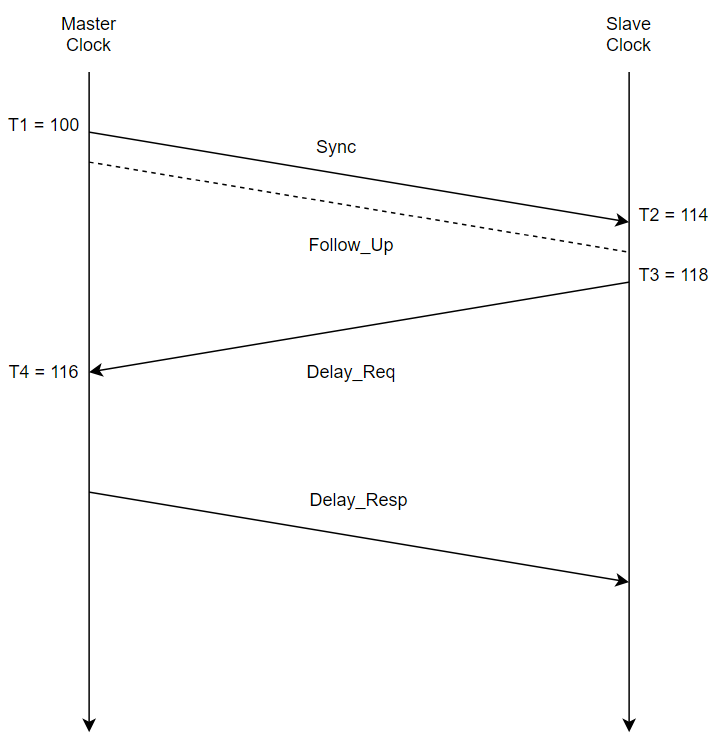
\includegraphics[width=0.8\textwidth]{First.png}
  \caption[Mecanismo E2E]{Mecanismo E2E}
  \label{fig:airbus1}
\end{figure}


Inserindo na equação 2.2 os valores dos tempos de envio e recepção das mensagens que estão definidos na figura, comprova-se o valor de 6 $\mu$s para o atraso no caminho. 

\[ Atraso =  \dfrac{(T4 - T1) - (T3 - T2)}{2} = \dfrac{(116 - 100) - (118 - 114)}{2} = 6\]

 Este procedimento para o cálculo do \textit{offsetFromMaster} formulado na versão inicial do PTP funciona com muito precisão quando o tempo de propagção da mensagen é igual nos dois sentidos, no entanto, incorre no problema causado pela presença de dispositivos intermédios já mencionado no capítulo introdutório.. Por exemplo, se houver congestionamento num dispositivo intermédio entre o \textit{Slave} e o \textit{Master} no momento em que por ele transita a mensagem \textit{Delay\_Req}, a mesma terá um tempo de propagação mais elevado do que a mensagem \textit{Sync}. Consequentemente, o atraso será erradamente calculado com a fórmula previamente apresentada, assim como os \textit{Local Clocks} serão imprecisamente sincronizados. Da mesma forma, o desfasamento entre o \textit{Master} e o \textit{Slave} também não será corretamente calculado se a mensagem \textit{Sync} for forçada a um atraso de propagação diferente daquele que foi previamente calculado com o mecanismo E2E. Para calcular corretamente os atrasos, o tempo de residência das mensagens nos dispositivos intermédios teria que ser registado e comunicado ao \textit{Slave}. As manipulações ás mensagens a efectuar pelos dispositivos intermédios para comunicar o tempo de residências das mensagens foram introduzidas no PTPV2. Ainda que as manipulações tenham alguns detalhes adicionais, em traços básicos, o tempo de residência nos \textit{Transparent Clocks} é adicionado ao campo \textit{correctionField} das mensagens e posteriormente subtraído pelo \textit{Slave} nos cálculos do atraso e \textit{offstedFromMaster}, obtendo-se as equações 2.3 e 2.4. 

\begin{equation}
    Atraso =  \dfrac{(T4 - T1) - (T3 - T2) - ResidenceTimeSync - 
    ResidenceTimeDelay\_Req}{2}
\end{equation}

\begin{equation}
    offsetFromMaster =  T2 - T1 - Atraso - ResidenceTimeSync
\end{equation}

Na figura 2.3 é apresentado um exemplo de como a implementação do suporte para funcionamento como \textit{Transparent Clcok} em dois dispositivos intermédios é usado para corrigir as assimetrias no tempo de propagação causadas por tempos de residência variáveis.


\begin{figure}[!htb]
  \centering
  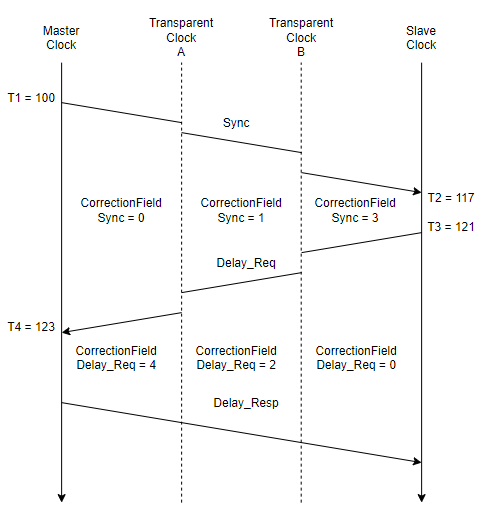
\includegraphics[width=0.8\textwidth]{correction.png}
  \caption[Aplicação do \textit{Transparent Clock}]{Aplicação do \textit{Transparent Clock}}
  \label{fig:airbus1}
\end{figure}


O exemplo é semelhante ao anterior, mas são descriminados dois \textit{Transparent Clocks} atravessados pelas várias mensagens que transitam entre o \textit{Slave} e o \textit{Master}. Além disso, é assumido que a mensagem \textit{Sync} é retardada por 1 $\mu$s no \textit{Transparent Clock} A e por 2 $\mu$s no \textit{Transparent Clock} B, e que a mensagem do tipo Delay\_Req demora 2 $\mu$s em cada um dos \textit{Transparent Clocks}. Como tal, é totalizado um valor de 3 $\mu$s para o \textit{CorrectionField} da mensagem \textit{Sync} quando esta chega ao \textit{Slave}, e de 4 $\mu$s para a mensagem \textit{Delay\_Req} quando esta chega ao \textit{Master}. 
Tal como no exemplo anterior, é assumido um desfasamento de 8 $\mu$s entre os \textit{Local PTP Clocks} e um tempo de propagação de 6 $\mu$s, e são apresentados os tempos de envio e recepção das mensagens \textit{Sync} e \textit{Delay\_Req}. Substituindo na equação 2.4 os instantes de tempo presentes no exemplo 
e os valores do \textit{CorrectionField} explicados, obtém-se o atraso de 6$\mu$s assumido.

\[ Atraso = \dfrac{(123 - 100) - (121 - 117) - 3 - 4}{2} = 6\]

\subsection{Mecanismo \textit{Peer-to-Peer}}

Alternativamente pode ser usado o mecanismo P2P para proceder à sincronização dos \textit{Local PTP Clocks}. Nesta variante, todos os dispositivos que participam na sincronização entre um \textit{Master} e um \textit{Slave} mantêm a informação do tempo de propagação de uma mensagem entre si e os seus vizinhos. Quando uma mensagem \textit{Sync} é enviada pelo \textit{Master}, todos os dispositivos intermédios adicionam ao \textit{CorrectionFieldSync} o tempo de residência no dispositivo e o tempo de propagação entre o dispositivo imediatamente anterior no caminho e si mesmo. Assim, quando a mensagem \textit{Sync} ou a respectiva mensagem \textit{Follow\_up} chegam ao \textit{Slave}, o atraso de propagação entre o \textit{Master} e o dispositivo imediatamente antes do \textit{Slave}, e todos os tempos de residência, já se encontram totalizados no \textit{CorrectionField}. Assím, para obter o \textit{Slave} obter o atraso entre si e o \textit{Master}, este apenas precisa de somar o atraso entre si e o seu vininho ao somatório dos restantes atrasos totalizados no \textit{correctionField} da mensagem \textit{Sync}. \par 
Por forma a obter os tempos de propagação entre dois vizinhos são trocadas mensagens do tipo \textit{PDelay\_Req}, \textit{PDelay\_Resp} e \textit{PDelay\_Resp\_Follow\_Up}. Um exemplo de cálculo do atraso de caminho está demonstrado na figura 2.4. Os valores do tempo de propagação e do desfasamento são os mesmos dos exemplos anteriores. 


No figura estão indicados os seguintes instantes de tempo:

\begin{itemize}
  \item T1  - \quad Instante de tempo de transmissão da mensagem \textit{PDelay\_Req} pelo \textit{Transparent Clock} A.
  \item T2  - \quad Instante de tempo de recepção da mensagem \textit{PDelay\_Req} pelo \textit{Transparent Clock} B. 
  \item T3  - \quad Instante de tempo de transmissão da mensagem \textit{PDelay\_Resp} pelo \textit{Transparent Clock} B.
  \item T4 - \quad Instante de tempo de recepção da mensagem \textit{PDelay\_Resp} pelo \textit{Transparent Clock} A.
\end{itemize}

O valor do atraso de caminho é obtido recorrendo à equeação 2.6:

\begin{equation}
    Atraso =  \dfrac{(T4 - T1) - (T3 - T2)}{2}
\end{equation}



Substituindo os instantes de tempo na equação 2.6, obtém-se 6 $\mu$s.

\[ Atraso =  \dfrac{(116 - 100) - (118 - 114)}{2} = 6\]

\begin{figure}[H]
  \centering
  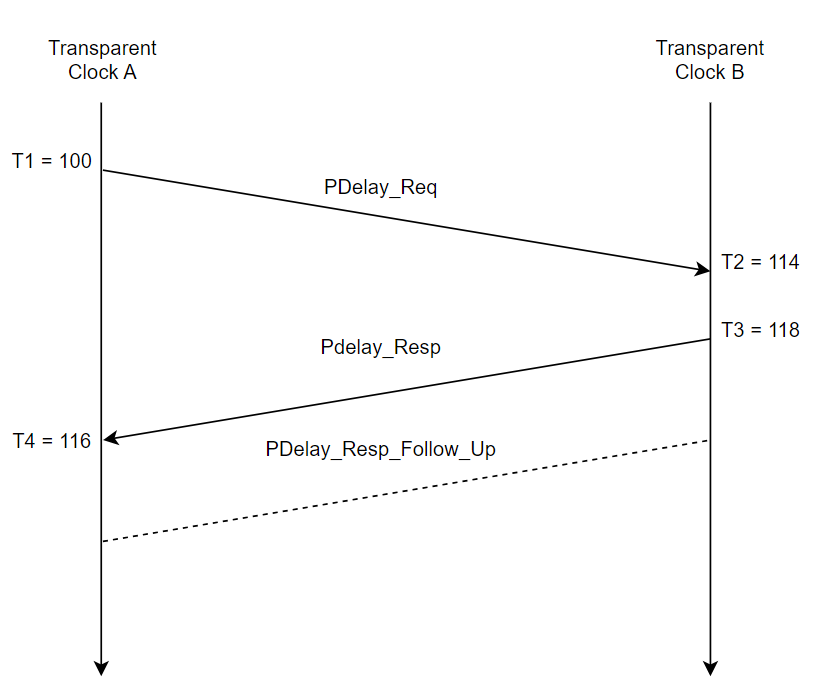
\includegraphics[width=0.8\textwidth]{Peed.png}
  \caption[Mecanismo P2P]{Mecanismo P2P}
  \label{fig:airbus1}
\end{figure}

\section{\textit{Power Utility Profile}}
\label{section:theory1}



O PTP pode ser implementado em redes construídas para funções variadas com diversos requisitos de desempenho.  Por forma a ajustar o PTP da melhor forma possível às características da rede na qual se recorre ao algoritmo, a norma dá liberdade a organizações relevantes em várias indústrias para que estas definam restrições a nível dos atributos e funcionalidades do PTP, aquando da sua implementação na respetiva indústria. À compilação destas variadas restrições dá-se o nome de perfil. Um perfil deve definir quais as opções do BMC que devem ser implementas, a utilização do mecanismo E2E ou P2P, os vários mecanismos de configuração da execução do protocolo, mecanismos de transporte, precisão e incerteza requerida ao nível da sincronização dos \textit{Clocks}, gamas de valores permitidas para os vários atributos do PTP, e as instâncias do PTP permitidas, requeridas ou proibidas. \par 

\iffalse
Por forma a integrar componentes que possam ser provenientes de diferentes fabricantes, foi criada a norma IEC 61850 que define protocolos de comunicação para dispositivos inteligentes em sistemas de automação de subestações elétricas (SAS) \cite{SAS}. A norma divide o SAS em três níveis:

\begin{itemize}
  \item \textit{Process Level} - Nível onde é feita aquisição de dados referentes ao vários equipamentos e estruturas da subestação, posteriormente enviados para os níveis superiores. É aqui que se encontram as \textit{Merging Units} (MU) e as \textit{Phasor Measurement Units}. 
  \item \textit{Bay level} - Nível onde se encontram vários \textit{Intelligent Electronic Devices} (IED), responsáveis por controlar individualmente os vários equipamentos da subestação. Além disso, encontram-se também neste nível equipamentos de segurança, como as relés de proteção.
  \item \textit{Station level} - É o nível mais próximo dos operadores das SAS. Inclui os sistemas SCADA (\textit{Supervisory Control and Data Acquisition}), que consistem num conjunto de equipamentos de \textit{hardware} e \textit{software}, utilizados para controlar e monitorizar a subestação com recurso a dados capturados no primeiro nível. Os operadores interagem com os sistemas SCADA através das \textit{Human Machine Interfaces} (HMI).
\end{itemize}

A arquitetura típica de um SAS que segue as regras definidas na norma IEC 61850 está ilustrada na figura 2.5.

\begin{figure}[H]
  \centering
  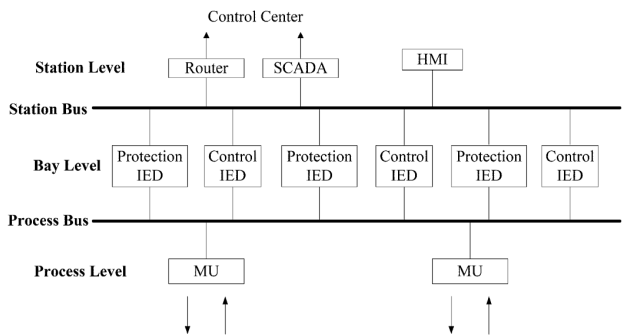
\includegraphics[width=1\textwidth]{SAS.png}
  \caption[Arquitetura típica de um sistema de automação de subestações elétricas ]{Arquitetura típica de um sistema de automação de subestações elétricas (fonte: \cite{comparison})}
  
  \label{fig:airbus1}
\end{figure}


\fi
Incluída na norma IEC 61850, a norma que define os protocolos de comunicação entre IEDs numa subestaçãoe elétrica, pode encontrar-se a subnorma IEEE 61850-9-3, vulgarmente denominada por \textit{Power Utility Profile} (PUP) \cite{PUP}, optimizada para fornecer a precisão de 1$\mu$s nas sincronizações, necessária para garantir a operacionalidade determinística dos sistemas críticos, sem inserir tráfego excessivo na rede e sem precisar de \textit{Boundary Clocks} excessivamente complexos.
O PUP exige que as comunicações sejam feitas sobre \textit{Ethernet}, com recurso exclusivamente ao mecanismo P2P e, preferencialmente, em modo de operação \textit{One-Way}, sem restrições ao nível do modo de operação do BMC. As mensagens usadas no protocolo devem recorrer sempre a tramas do tipo \textit{multicast}. Com a escolha do mecanismo P2P, o \textit{GrandMaster} da rede apenas comunica com o \textit{Transparent Clock} com o qual tem uma ligação. Assim, é possível aumentar a quantidade de dispositivos na rede a sincronizarem-se, em última instância, com o \textit{GrandMaster}, sem que para isso o mesmo precise de processar uma maior quantidade de tráfego. O PUP tem ainda a vantagem de ser compatível com protocolos que assegurem a resiliência da rede face a falhas singulares de elementos na mesma, tais como o \textit{Parallel Redundancy Protocol} (PRP) \cite{PRP}, e o \textit{High-availability Seamless Redundancy} (HSR) \cite{HSR}. Por forma a cumprir com a precisão de 1 $\mu$s, necessária em subestações elétricas, o PUP define as seguintes imprecisões máximas aceitáveis nos vários elementos na rede:  

\begin{itemize}
  \item \textit{GrandMaster Clock} - 250 ns
  \item \textit{Boundary Clock} - 200 ns
  \item \textit{Transparent Clock} - 50 ns
\end{itemize}

As imprecisões definidas permitem alcançar o desempenho requerido numa situação em que as mensagens tenham que atravessar até 15 \textit{Transparent Clocks} para se deslocarem do \textit{GrandMaster} com destino a um \textit{Slave}. O PUP exige ainda a transmissão periódica, com intervalos de 1 s, das mensagens do tipo \textit{Announce}, \textit{Sync} e \textit{PDelay\_Req}. As mensagens \textit{Announce} devem ser descartadas quando circulam por mais de 3 s na rede. 

\iffalse

\par Na figura 2.6 encontra-se ilustrado um exemplo de uma rede onde um \textit{switch} de \textit{Ethernet} é usado como \textit{Transparent Clock} para contribuir para a sincronização dos vários elementos de uma SAS com um \textit{Grandmaster}.

\begin{figure}[H]
  \centering
  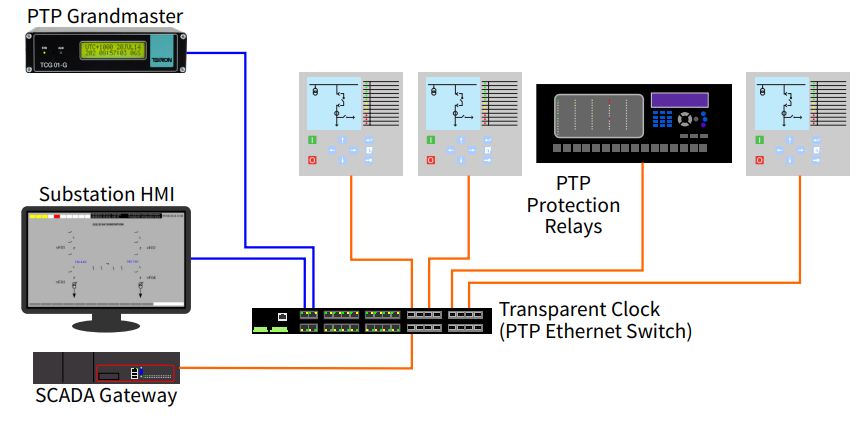
\includegraphics[width=1\textwidth]{topology.png}
  \caption[Rede numa SAS sincronizada via PTP ]{Rede numa SAS sincronizada via PTP (fonte: \cite{Electrical})}
  \label{fig:airbus1}
\end{figure}

\fi

\section{Implementação de um \textit{Transparent Clock}}

O comutador a desenvolver deverá, numa primeira fase, atuar como \textit{Transparent Clock}, podendo ser posteriormente adicionado o suporte para um funcionamento misto como \textit{Transparent Clock} e \textit{Boundary Clock}. Mais ainda, ainda que o PUP apenas imponha a suporte do mecanismo P2P, tanto este como o E2E serão implementados. 

\subsection{Processamento das mensagens}

As instâncias do PTP são postas em prática através da manipulação das mensagens já explicadas, substituindo os vários campos do corpo e cabeçalho das mesmas por instantes de tempo de envio e recepção de mensagens e demais dados armazenados na instância. Os vários campos de dados presentes nos cabeçalhos das várias mensagens do PTP são os seguidamente referidos.  

\begin{itemize}
  \item \textit{versionPTP}  - \quad Identificador da versão do PTP em execução no domínio. 
  \item \textit{\textit{domainNumber}} - \quad Mecanismo primordial para isolamento e identificação de um domínio por parte de utilizadores e dispositivos.
  \item \textit{\textit{sdoId}}  - \quad Campo que transmite informação relativa à identificação do domínio em complementaridade com o campo \textit{domainNumber}.
  \item \textit{messageType} - \quad Identificador do tipo de mensagem.
  \item \textit{flagField}  - \quad Campo no qual os vários bits funcionam como sinalizadores de propriedades da execução do PTP por parte das instâncias envolvidas na transmissão da mensagem.
  \item \textit{correctionField}  - \quad Campo que, como explicado num capítulo anterior, transmite informação relativa aos instantes de tempo de transmissão e recepção de mensagens da classe evento.
  \item \textit{sourcePortIdentity} - \quad Identificador do porto PTP percecionado como originador da mensagem.
  \item \textit{sequenceId}  - \quad Identificador usado para coordenar o envio de mensagens da classe evento e a aplicação da informação das mesmas nos cálculos dos atrasos e desfasamentos. 
  \item \textit{logMessageInterval}  - \quad Campo que pode transmitir informação relativa à periodicidade requerida de envio de mensagens dos vários tipos.
\end{itemize}

No que diz respeito ao corpo das mensagens, estão definidos na norma os campos de dados apresentados na tabela 5.1:


\begin{table} [H]
\begin{center}
\begin{tabular}{|l| l|l|}

    \hline
    Mensagem & Campo de Dados & Conteúdo \\
    \hline
     \textit{Sync} & \textit{originTimestamp} & Instante de transmissão da mensagem \textit{Sync} \\
    \hline
    \multirow{2}{*}{\textit{Follow\_Up}} & \multirow{2}{*}{\textit{preciseOriginTimestamp}} & Instante de transmissão da mensagem \textit{Sync} correspondente  \\
    & & em modo \textit{Two-Way} \\
    \hline
    \textit{Delay\_Req} & \textit{originTimestamp} & Instante de transmissão da mensagem \textit{Delay\_Req} \\
    \hline
    \multirow{3}{*}{\textit{Delay\_Resp}} & \textit{receiveTimestamp} & Instante de recepção
    da mensagem \textit{Delay\_Req} no \textit{Master}\\
    \cline{2-3}
    & \multirow{2}{*}{\textit{requestingPortIdentity}}  &  Campo que transmite a identificação do porto que enviou a \\
    &   &  mensagem \textit{Delay\_Req} à qual se está a responder\\
    \hline
    \textit{PDelay\_Req} & \textit{originTimestamp} & Instante de transmissão da mensagem \textit{PDelay\_Req} \\
    \hline
     \multirow{3}{*}{\textit{PDelay\_Resp}} & \textit{requestReceiptTimestamp} & Instante de recepção
    da mensagem \textit{PDelay\_Req} \\
    \cline{2-3}
    & \multirow{2}{*}{\textit{requestingPortIdentity}}  &  Campo que transmite a identificação do porto que enviou a \\
    &   &  mensagem \textit{PDelay\_Req} à qual se está a responder\\
    \hline
    & \multirow{2}{*}{\textit{responseOriginTimestamp}} & Instante de transmissão da mensagem \textit{PDelay\_Resp}  \\
    \textit{PDelay\_Resp}& & correspondente em modo \textit{Two-Way} \\
    \cline{2-3}
    \textit{\_Follow\_Up}& \multirow{2}{*}{\textit{requestingPortIdentity}}  &  Campo que transmite a identificação do porto que enviou a \\
    &   &  mensagem \textit{PDelay\_Req} à qual se está a responder\\
    \hline
    
    \hline
\end{tabular}
\end{center}
\caption{Campos de dados das mensagens}\label{Campos de dados das mensagens}
\end{table}


A execução do PTP decorre sobre a divisão lógica de uma rede em domínios. Por forma a isolar os diferentes domínios numa mesma rede, todas as mensagens que circulam num domínio devem ter a mesma combinação dos parâmetros \textit{sdoId} e \textit{domainNumber}, que devem diferir entre os vários domínios. No momento de recepção de uma mensagem por parte de uma instância, uma mensagem apenas deve ser considerada para posterior processamento e reencaminhamento quando os respetivos campos \textit{sdoId} e \textit{domainNumber} correspondem com aqueles guardados internamente nas estruturas de dados das instâncias. \par
Uma descrição detalhada do procedimento a adotar pelo comutador aquando da recepção dos vários tipos de mensagens é apresentada seguidamente.

\textbf{\textit{Sync}} Aquando da recepção de uma mensagem \textit{Sync} o comutador deve adicionar ao \textit{correctionField} da mesma o tempo de residência e, no modo P2P, o tempo de propagação entre si e o último dispositivo com suporte para o mecanismo P2P que manipulou a mensagem. \par

\textbf{\textit{Follow\_Up}} A mensagem deve ser reencaminha sem proceder a manipulações da mesma. \par

\textbf{\textit{Delay\_Req}} A mensagem deve ser descarta em modo P2P. Em modo E2E deve ser reencaminha em modo \textit{broadcast} e adicionado o tempo de residência da mensagem ao \textit{correctionField} da mesma. \par

\textbf{Delay\_Resp} A mensagem deve ser tratada da mesma forma que a mensagem \textit{Delay\_Req}. \par

\textbf{\textit{PDelay\_Req}} Aquando da recepção de uma mensagem \textit{PDelay\_Req} em modo P2P, se a mesma passar as validações necessárias, deverá ser preparada uma mensagem do tipo \textit{PDelay\_Resp} para envio o mais prontamente possível. O \textit{Sequence Id} e o \textit{sourcePortIdentity} da mensagem \textit{PDelay\_Req} devem ser inseridos respetivamente nos campos \textit{sequenceId} e \textit{requestingPortIdentity} da mensagem \textit{PDelay\_Resp}. Esses dois campos serão posteriormente analisados pelo criador da mensagem \textit{PDelay\_Req}, por forma a concluir que a \textit{PDelay\_Resp} é enviada em resposta precisamente à sua mensagem \textit{PDelay\_Res}. O \textit{correctionField} deverá ser o somatório entre o \textit{correctionField} da mensagem \textit{PDelay\_Req} e a diferença entre o instante de transmissão da mensagem \textit{PDelay\_Resp} e de transmissão da mensagem \textit{PDelay\_Req}. Por sua vez, em modo E2E, deverá ser reencaminhada em modo \textit{broadcast}, e adicionado o tempo de residência no \textit{Transparent Clock} ao \textit{correctionField} da mesma.

\textbf{\textit{PDelay\_Resp}} A mensagem deverá ser descartada quando o modo de operação é P2P. No entanto, quando o conteúdo da mensagem se encontra em conformidade com o devido quando a mensagem se destina ao \textit{Transparent Clock}, deverão ser acionados os cálculos do tempo de propagação entre o \textit{Transparent Clock} e a instância que criou a mensagem. Em modo E2E, deverá ser reencaminhada em modo \textit{broadcast}, e adicionado o tempo de residência ao \textit{correctionField} da mesma. 

\textbf{\textit{PDelay\_Resp\_Follow\_Up}} Tal como na recepção de uma mensagem \textit{PDelay\_Resp} em modo P2P, a mensagem deverá ser descartada, ainda que possa acionar os cálculos do tempo de propagação. Em modo E2E, deverá ser reencaminhada em modo \textit{broadcast}, e adicionado o tempo de residência no \textit{Transparent Clock} ao \textit{correctionField} da mesma.

\textbf{\textit{Management}} A mensagem deverá ser reencaminhada ou, se tiver o \textit{Transparent Clock} como destinatário, ser descartada. \par

\textbf{Signaling} Tal como a mensagem \textit{Management}, deverá ser reencaminhada ou descartada quando o \textit{Transparent Clock }for o seu destinatário. \par

\subsection{Cálculo do atraso}

O cálculo do tempo de propagação entre os vários PTP \textit{ports} do \textit{Transparent Clock} e as instâncias vizinhas com suporte para o mecanismo P2P ocorre aquando da recepção de uma mensagem \textit{PDelay\_Resp}, ou da respetiva \textit{PDelay\_Resp\_Follow\_Up} num porto a operar no modo P2P, e deverá ser guardado na estrutura de dados denominada de \textit{meanLinkDelay}. Aquando da recepção de uma mensagem \textit{PDelay\_Resp}, é verificado o valor de um bit específico do campo \textit{flagField} da mesma, denominado \textit{twoStepFlag}. Quando este bit vem a 0, significa isto que a instância responsável por enviar a mensagem está a operar no modo \textit{One-Way} e que a totalidade da informação gerada pela respetiva instância necessária para calcular o tempo de propagação já se encontra incluída na mesma. Consequentemente, o tempo de propagação é calculado com a fórmula 5.1, onde t1 representa o instante de recepção da mensagem \textit{PDelay\_Resp}, e t4 o instante de transmissão da mensagem \textit{PDelay\_Req}.

\begin{equation}
    meanLinkDelay = \dfrac{(t4 - t1) - PDelay\_RespCorrectionField}{2} 
\end{equation}

Inversamente, quando o \textit{twoStepFlag} tem o valor 1, a instância que gerou a mensagem \textit{PDelay\_Resp} está a operar no modo de funcionamento \textit{Two-Way}. Devido a isso, a informação do instante de transmissão da mensagem \textit{PDelay\_Resp} não se encontra na mesma e não é disponibilizada ao \textit{Transparent Clock}. Assim, o \textit{Transparent Clock} não procede aos cálculos do tempo de propagação, esperando pela chegada de uma mensagem \textit{PDelay\_Resp\_Follow\_Up} com o mesmo \textit{sequenceId} da mensagem \textit{PDelay\_Resp}. No momento de recepção da mesma, o tempo de propagação é calculado com a fórmula 4.2.




    \begin{equation}
    \begin{split}
         meanLinkDelay = & ((t4 - t1) - (responseOriginTimestamp -requestReceiptTimestamp ) \\ & - PDelay\_RespCorrectionField - \\ 
    & PDelay\_Resp\_Follow\_UpCorrectionField) / 2
    \end{split}
    \end{equation}
    

\subsection{Estrutura interna}

\iffalse
Para uma correta execução das funcionalidades fundamentais do protocolo é apenas exigido às instâncias que manipulem e enviem as mensagens como definido na norma quando a comunicar com instâncias que não foram especialmente desenvolvidas para comunicar entre si. No entanto, entre duas instâncias vizinhas, estas podem proceder a uma comunicação com regras e técnicas próprias se para isso forem previamente desenvolvidas, e essa comunicação poder ser escondida das restantes instâncias. Tais situações estão previstas na norma, por isso, é dada bastante liberdade de escolha na execução do PTP e implementação das instâncias.\par
\fi
Ainda que esta não tenha que ser estritamente seguida, a norma sugere qual deve ser a estrutura interna dos vários tipos de instância, tais como os \textit{Transparent Clocks}. Os vários módulos cuja implementação é sugerida são os seguidamente referidos. \par 


\textbf{\textit{Network Interface Stack}} Módulo responsável por capturar os instantes de tempo de recepção e transmissão das mensagens da classe evento.

\textbf{PTP \textit{Port Block}} Módulo responsável pelas funcionalidades de um PTP \textit{Port} que não sejam dependentes das regras do meio de comunicação. Entre outras funções deve manter as estruturas de dados referentes a um PTP\textit{Port} e gerar as mensagens da classe evento. 

\textbf{PTP \textit{Common Core}} É sugerido o desenvolvimento de um módulo central que comunique com os vários PTP \textit{Ports} presentes na instância. Este deve ser responsável por gerenciar as estruturas de dados presentes na instância que não se restrinjam a um único PTP \textit{Port} e providencia-las aos mesmos. No caso de \textit{Ordinary Clocks} e \textit{Boundary Clocks} deve ainda ser responsável por aspetos do BMC que requeiram informação dos vários PTP \textit{Ports}.

\textbf{\textit{Media Dependent Adapter}} Para dar a uma mensagem o formato adequado ao meio de comunicação onde se encontra a instância é sugerido este módulo. No caso da implementação de um dispositivo numa rede \textit{Ethernet}, o módulo deve inserir a mensagem no campo de dados de uma trama e preencher os restantes campos adequadamente. % file "Thesis_Background.tex"
\cleardoublepage

%%%%%%%%%%%%%%%%%%%%%%%%%%%%%%%%%%%%%%%%%%%%%%%%%%%%%%%%%%%%%%%%%%%%%%%%
%                                                                      %
%     File: Thesis_Implementation.tex                                  %
%     Tex Master: Thesis.tex                                           %
%                                                                      %
%     Author: Andre C. Marta                                           %
%     Last modified : 13 May 2019                                      %
%                                                                      %
%%%%%%%%%%%%%%%%%%%%%%%%%%%%%%%%%%%%%%%%%%%%%%%%%%%%%%%%%%%%%%%%%%%%%%%%



\chapter{Fundamentos de um switch}
\label{chapter:implementation}
\section{LAN e MAC \textit{bridge}}
A Ethernet foi introduzida em 1973 pelo grupo de trabalho IEEE 802.3 com o propósito de interligar computadores e outros dispositivos em redes de área local (LAN). LAN são redes que interconectam computadores numa área limitada como um campus ou um escritório. Nestas, os vários dispositivos têm um endereço físico que deve ser único na rede, denominado de endereço MAC. \par 
Um dispositivo genericamente denominado de \textit{bridge} é usado para agregar segmentos de uma LAN ou um conjunto de LANs. As regras que devem ser seguidas pelas \textit{bridges} foram definidas na norma IEEE 802.1D  \cite{Bridge}. As \textit{bridges} possuem o mínimo de dois pontos de acesso a canais de comunicação da rede, denominados de portos, e reencaminham pacotes de informação entre os mesmos. A estes pacotes chama-se tramas e o seu formato varia consoante a tecnologia em que esteja implementada a LAN. \par 
As \textit{bridges} possuem uma tabela que faz a associação entre os vários endereços MAC do seu conhecimento e os portos das mesmas que estão interligados com o dispositivo com o respectivo endereço. No momento de receção de uma trama, a \textit{bridge} faz uma procura pelo endereço MAC de destino presente no cabeçalho da trama. Se o endereço for encontrado e o porto associado não coincidir com o porto de receção da trama, a mesma é transmitida para o porto associado, denominando-se de envio \textit{unicast}. Contrariamente, se o endereço não for encontrado, a trama é enviada por todos os restantes portos, denominando-se o envio de \textit{broadcast}. Por sua vez, o endereço de origem presente no cabeçalho pode ser adicionado à tabela juntamente com o porto de receção.

\par Na figura 3.1 está ilustrada uma LAN com 8 computadores e uma \textit{bridge} juntamente com o preenchemento da tabela de endereços do mesmo.



\begin{figure}[H]
  \centering
  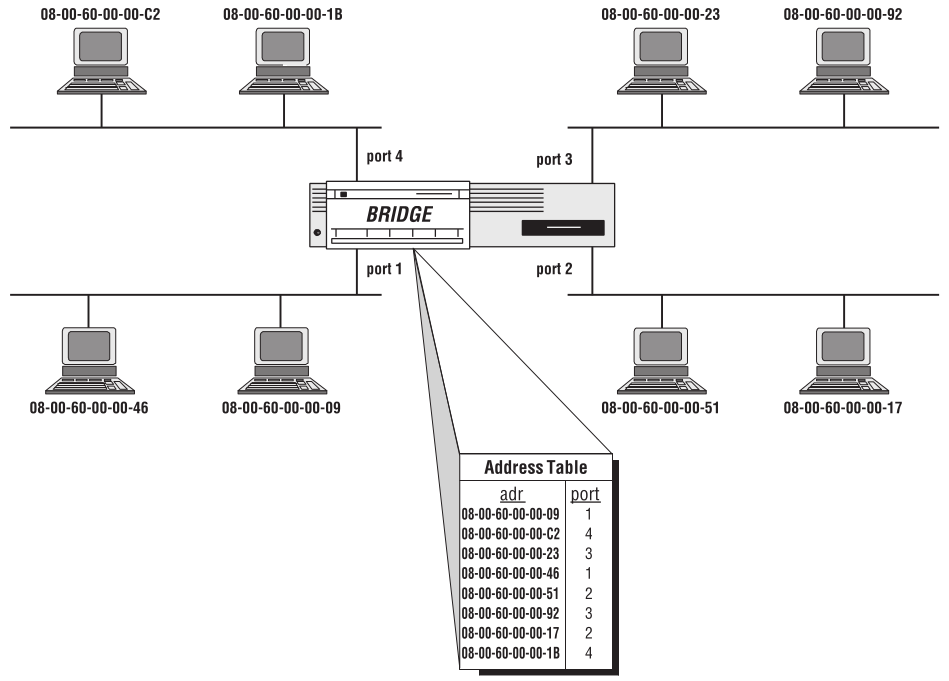
\includegraphics[width=1\textwidth]{Bridge.png}
  \caption[MAC bridge]{MAC \textit{bridge} \cite{make}}
  \label{fig:airbus1}
\end{figure}

\subsection{LAN virtual}

Na norma IEEE 802.1Q foi introduzido o conceito de LAN virtual (VLAN). Estas consistem numa divisão de uma rede fisicamente interligada num conjunto de LANs logicamente separadas. Numa VLAN, os seus membros apenas trocam informação com outros membros da mesma VLAN ainda que possa haver caminhos disponíveis para comunicar com membros de outras VLANs. As VLAN permitem aumentar a escalabilidade de uma rede, facilitar a mobilidade dos elementos da rede, aumentar a segurança e diminuir o tráfego desnecessário na mesma. \par

A sepração da rede em VLAN é implementada com recurso a switches com a capacidade de identificar a VLAN a que uma trama pertence e de usar essa informação na decisão do reencaminhamento da trama. A identificação da VLAN a que a trama pertence é efectuada com recurso à etiqueta VLAN que pode estar incluíada na trama. Esta tem a dimensão de dois octetos e está dividida nos seguintes 4 campos:

\begin{itemize}
  \item \textit{Tag Protocol Identifier}  - \quad Um código com a dimensão de um octeto que sinaliza a inclusão da etiqueta na trama.
  \item \textit{Priority Code Point}  - \quad Três bits que indicam a prioridade de transmissão da trama. Este campo não está diretamente associado à gestão das VLAN vai foi inserido na etiqueta por conveniência.
  \item \textit{Drop Eligeble Indicator}  - \quad Um bit que dá indicação de se a trama pode ser descartada em caso de congestionamento. Tal como o campo anterior foi inserido na etiqueta por conveniência.
  \item VLAN \textit{Identifier}  - \quad Identificador da VLAN à qual a trama pertence com a dimensão de doze bits. 
  \end{itemize}

  Quando a etiqueta não vem incluída na trama o switch pode identificar a VLAN a que esta pertence com recurso a diferentes estratégias. A mais comum e apoiada pela norma IEEE 802.1Q é a associação por porto. Nesta o switch mantém uma lista de da VLAN a que conecta cada um dos seus portos. 
  Um exemplo da associação de VLAN a portos está ilustrada na figura 3.2

  
\begin{figure}[H]
  \centering
  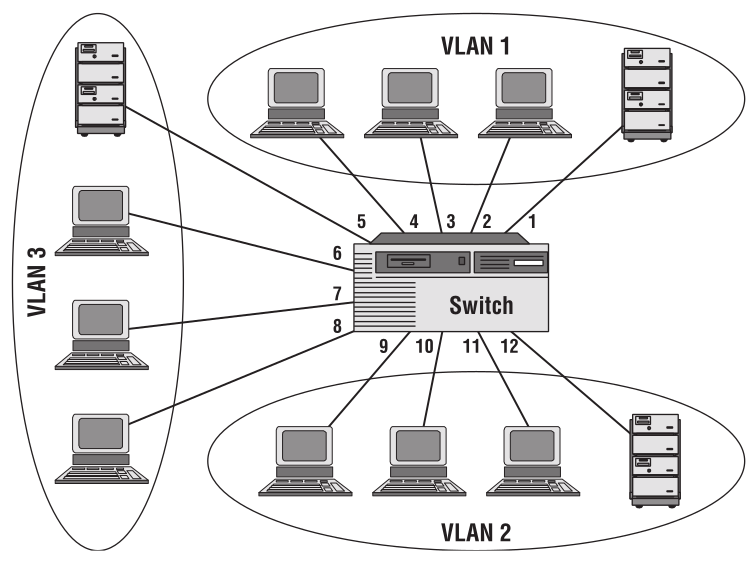
\includegraphics[width=0.7\textwidth]{Port_ASS.png}
  \caption[Associação porto-VLAN]{Associação porto-VLAN}
  \label{fig:airbus1}
\end{figure}

A tabela a consultar no momento da receção da trama para identificação da VLAN corrrespondente pode ser preenchida estaticamente ou dinamicamente com recurso a protocolos como o GARP. \par




\subsection{\textit{Spanning tree protocol}}


\section{\textit{Ethernet}}
\label{section:model}
 A Ethernet foi introduzida em 1973 pelo grupo de trabalho IEEE 802.3 com vista à sua utilização em redes LAN. Devido à sua simplicidade, baixo-custo e padronização de implementação, ganhou preponderância globalmente e foi a sua utilização foi extendida a redes de mais vasta área geográfica. Na atualidade, a maioria do tráfego da internet é gerado a partir de redes \textit{Ethernet}. Na sua versão primordial, a \textit{Ethernet} tinha débitos de 10 Mbps em ligações \textit{half-duplex}, sobre uma topologia \textit{bus} com o dispositivo conhecido como Ethernet \textit{Hub} a funcionar como \textit{bridge}. Tal significava que vários dispositivos partilhavam um único canal de comunicação, tendo que dividir o débito do canal entre si. De forma a gerenciar os acessos ao canal, implementava-se o mecanismo \textit{carrier-sense multiple access}. Posteriormente, com o aparecimento de tecnologias com maior débito como \textit{Fast Ethernet} e \textit{Gigabit Ethernet}, os \textit{Ethernet Hubs} foram substituídos por switches e as ligações \textit{half-duplex} por ligações \textit{full-duplex} segundo uma topologia em estrela, ganhando a designação comum de \textit{Switch-Ethernet}, devido à centralidade do referido dispositivo no funcionamento da rede. \par 
 
 \subsection{Trama de Ethernet}
 
Atualmente existem alguns tipos de tramas diferentes, divididas em vários campos de dados, consoante a norma aplicável. A versão mais predominante é a \textit{Ethernet} II. Nesta versão, os vários campos das tramas, as suas regras e conteúdo são os seguintes: 

\begin{itemize}
  \item Preâmbulo  - \quad Não pertence diretamente à trama, servindo como sinal para que o dispositivo que a recebe sincronize o seu ciclo de relógio ao canal de transmissão. É constituído por sete bytes consecutivos com o valor 10101010. 
  \item \textit{Start Frame Delimiter} (SFD)  - \quad Tal como o preâmbulo, não pertence diretamente à trama, sendo usado para sinalizar o início do envio da trama. É constituído por um byte com o valor 10101011.  
  \item Origem  - \quad Campo com a dimensão de 6 bytes, portador do endereço MAC do dispositivo que iniciou o envio da trama.
  \item Destino - \quad Campo com a dimensão de 6 bytes, portador do endereço MAC do dispositivo ao qual se destina a trama.
  \item IEEE 802.1Q -\quad Etiqueta VLAN explicada previamente que pode ser incluída na trama.
  \item \textit{EtherType} - \quad Campo que transmite a informação relativa ao campo de dados da trama. O valor deste campo deve ser superior a 1536, e indica o protocolo de mais alto nível que encapsula o campo de dados. No caso do PTP este campo tem o valor 0x88F7. Noutras normas, como o IEEE 802.3, este campo pode ter um valor inferior a 1500 e transmite o comprimento do campo de dados.
  \item \textit{Payload} - \quad Campo que contém os dados a serem transmitidos na rede. No caso do PTP, o cabeçalho, corpo e, quando existam, TLVs de uma mensagem são inseridos no \textit{Payload} da trama.
  \item \textit{Frame Check Sequence} (FCS). -\quad Campo que contém os 4 bytes de um código gerado pelo último dispositivo que manipulou a trama e afixado no final da mesma. No dispositivo que recebe a trama e nos switches que a retransmitem, o código é calculado novamente, e caso não coincida com o FCS incluido na trama, significa que esta sofreu erros. O FCS pode ser gerado de várias formas, mas tipicamente consiste num \textit{Cyclic Redundant Check} (CRC). 

  

\begin{figure}[H]
  \centering
  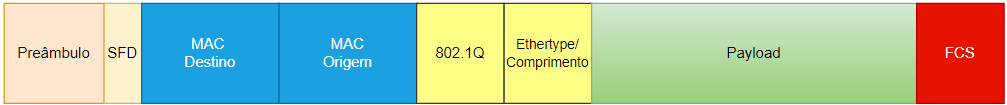
\includegraphics[width=1.\textwidth]{trama_best.png}
  \caption[Trama de Ethernet]{Formato de uma trama}
  \label{fig:airbus1}
\end{figure}


  
\end{itemize}


\subsection{\textit{Cyclic Redundancy Check}}


A norma IEEE 802.1D impôe a implementação de uma mecanismo de verificação de erros em tramas, ou seja, o FCS previamente mencionado. Em Ethernet é usado um \textit{Cyclic Redundant Check} (CRC). Este faz parte da classe de código cíclicos. O CRC é calculado pelo dispositivo que gera a trama e inserido no campo FCS. Aquando da receção da trama noutro disposito, o CRC deve ser novamente calculado. Quando CRC calculado coincide com o que vem na trama é considerado que esta está ausente de erros. Contrariamente, caso não coincidam, a norma IEEE 802.1D impõe que a trama seja descartada devido a provavel presença de erros na mesma.\par
O código CRC é o resto da divisão módulo 2 da trama acrescida de 4 octetos nulos por um polinómio de grau 32 sobre um campo finito de dois elementos. Devido à propriedade de as subtrações serem iguais às somas em campos finitos de dois elementos, a adição do CRC à trama garante que esta passa a ser divisível pelo polinómio gerador do CRC. Daí resulta que calcular o CRC da totalidade de uma trama recebida num dispositivo deve produzir 32 bits com o valor 0.\par
A divisão de dois polinómio em campos finitos de dois elementos pode ser efectuada iterativamente através da subtração de múltiplos do divisor sobre o dividendo. As subtrações, por sua vez, são iguais ás somas. Seguidamente são detalhados as etapas a efectuar numa iteração da divisão. 

\begin{enumerate}
\item Multiplicar o divisor por \(x^{n}\). O índice n na primeira iteração é igual à diferença entre o expoente máximo do dividendo e o expoente máximo do divisor.
\item Subtrair o dividendo pelo produto do divisor por \(x^{n}\).
\item Se n igual a 0, finalizar o algoritmo. Caso contrário, decrementar n.
\end{enumerate}

Na tabela 3.1 é dado o exemplo da divisão do polinómio \(x^{9} + x^{8} + x^{7} + x^{6} + x^{5}\) por \(x^{3} + x^{1}\) com o algoritmo descrito.


\begin{table}[H]
\begin{center} 
\begin{tabular}{|l l l l l l l l l l|}

    \hline
    \rowcolor{lightgray}
    1 & 1 & 1 & 1 & 1 & 0 & 0 & 0 & 0 & 0 \\
    \cellcolor{green}1 & \cellcolor{green}0 & \cellcolor{green}1 & \cellcolor{green}0 & & & & & & \\
    \hline
    \rowcolor{lightgray}
    0 & 1 & 0 & 1 & 1 & 0 & 0 & 0 & 0 & 0 \\
    & \cellcolor{green}1 & \cellcolor{green}0 & \cellcolor{green}1 & \cellcolor{green}0 & & & & &\\
    \hline
    \rowcolor{lightgray}
    0 & 0 & 0 & 0 & 1 & 0 & 0 & 0 & 0 & 0 \\
    & & \cellcolor{red}1 & \cellcolor{red}0 & \cellcolor{red}1 & \cellcolor{red}0 & & & & \\
    \hline
    \rowcolor{lightgray}
    0 & 0 & 0 & 0 & 1 & 0 & 0 & 0 & 0 & 0 \\
    & & & \cellcolor{red}1 & \cellcolor{red}0 & \cellcolor{red}1 & \cellcolor{red}0 & & & \\
    \hline
    \rowcolor{lightgray}
    0 & 0 & 0 & 0 & 1 & 0 & 0 & 0 & 0 & 0 \\
    & & & & \cellcolor{green}1 & \cellcolor{green}0 & \cellcolor{green}1 & \cellcolor{green}0 & & \\
    \hline
    \rowcolor{lightgray}
    0 & 0 & 0 & 0 & 0 & 0 & 1 & 0 & 0 & 0 \\
    & & & & & \cellcolor{red}1 & \cellcolor{red}0 & \cellcolor{red}1 & \cellcolor{red}0 & \\
    \hline
    \rowcolor{lightgray}
    0 & 0 & 0 & 0 & 0 & 0 & 1 & 0 & 0 & 0 \\
    & & & & & & \cellcolor{green}1 & \cellcolor{green}0 & \cellcolor{green}1 & \cellcolor{green}0 \\
    \hline
    \cellcolor{lightgray}0 & \cellcolor{lightgray}0 & \cellcolor{lightgray}0 & \cellcolor{lightgray}0 & \cellcolor{lightgray}0 & \cellcolor{lightgray}0 & \cellcolor{blue}0 & \cellcolor{blue}0 & \cellcolor{blue}1 & \cellcolor{blue}0 \\
    \hline
    
\end{tabular}
\end{center}

\end{table}


Na primeira iteração do processo de divisão o divisor é multiplicador por \(x^{6}\) resultando no polinómio \(x^{9} + x^{7}\). Por sua vez, ese resultado é subtraido no dividendo obtendo-se o polinómio \(x^{8} + x^{6} + x^{5}\) que é usado como dividendo na seguinte iteração. No final do algoritmo é obtido, como resto da divisão, o polinómio \(x^{1}\) que pode ser representado binariamente como 010. \par
O algoritmo demonstrado é de fácil implementação em RTL, o que contribuiu para a utilização do CRC como método de deteção de erros em Ethernet.  



\section{Componentes}
\label{section:model}

O switch de \textit{Ethernet} é uma classe de dispositivos de elevada complexidade. Um switch além de receber e enviar tramas, deve também ser capaz de aprender enquanto membro de uma rede, quais os portos que levam as tramas a chegar aos destinos desejados, verificar a ocorrência de erros, seguir as regras de VLAN, proceder ao processamento, criação e alteração de tramas segundo protocolos de alto nível e, como é o caso no PTP, participar ativamente na execução dos protocolos. Para isso, as arquitecturas dos switches são divididas em vários módulos, cada qual responsável por executar uma tarefa específica dentro das várias necessárias no dispositivo. Alguns módulos podem estar ou não presentes e seguir abordagens distintas consoante as arquitecturas que sejam escolhidas na utilização que se pretende para o switch. No entanto, alguns componentes são fundamentais e devem servir como base no desenvolvimento de um switch. Dois desses componentes vitais a um switch são a tabela de endereços e a \textit{switch fabric} \cite{make}. \par
\subsection{Lógica de reencaminhamento}
A procura, inserção e eliminação de elementos da tabela pode ser implementada com diferentes abordagens, variando em eficácia, eficiência temporal, eficiência de utilização de memória, quantidade de \textit{hardware} necessário e complexidade no desenvolvimento e, em última análise, em custo monetário. As duas formas mais comuns de implementar o processamento da tabela é com recurso a algoritmos de procura semelhantes aos usados em \textit{software}, ou, quando possível, com recurso a memórias CAM (\textit{Content Addressable Memory}) \cite{CAM}. As memórias CAM são um tipo de memória muito usado em redes de computadores e em aplicações que exijam uma elevada eficiência temporal. O seu modo de operação consiste em serem capazes de devolver o endereço de memória de um conjunto de bits que estejam armazenados na mesma em apenas um ciclo de relógio. Para o conseguirem, as células de uma memória CAM, que armazenam um bit de informação, têm um circuito semelhante ao de uma célula SRAM, à qual são adicionados quatro transístores para funcionarem como comparadores entre o conteúdo de uma célula e os bits de uma palavra que se procura na CAM. O circuito básico pode ser observado na figura 3.3. Os transístores M1, M2, M3 e M4 são responsáveis pela comparação entre D, o bit armazenado, e SL, o bit da palavra. O par de transístores M1 e M3, tal como o par M2 e M4 funcionam como um caminho entre ML e a terra. Quando SL e D têm valores opostos, ou seja, o bit que se procura difere do bit armazenado, um dos dois caminhos conduz corrente forçando ML a ficar com a tensão de terra. Contrariamente, se houver correspondência entre D e SL, os caminhos não conduzem, desconectando ML da terra.  Quando ML é desconectado em todas as células que armazenam os bits de uma palavra, um sinal com o valor lógico 1 é introduzido num codificador levando a que a saída do mesmo seja o endereço de memória da palavra que se procurava. Um exemplo de uma \textit{CAM} que armazena palavras de 3 bits pode ser observado na figura 3.2.

\begin{figure}[H]
\centering
\begin{minipage}{.5\textwidth}
  \centering
  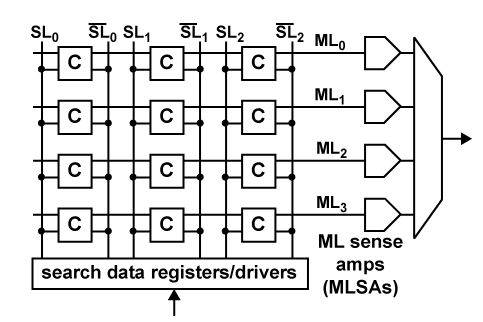
\includegraphics[width=.9\linewidth]{CAM_TOP.png}
  \caption{Memória CAM}{(fonte: \cite{CAM})}
  \label{fig:test1}
\end{minipage}%
\begin{minipage}{.5\textwidth}
  \centering
  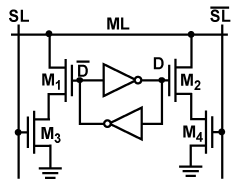
\includegraphics[width=.7\linewidth]{CAM.png}
  \caption{Célula CAM}{(fonte: \cite{CAM})}
  \label{fig:test2}
\end{minipage}
\end{figure}

Desenvolvendo as CAM com recurso a uma arquitectura de muito baixo nível é possível obter uma excelente eficiência na procura sem ser necessário pagar o custo de complexidade ao nível lógico. Em situações em que não seja possível incluir uma CAM abordada da forma descrita, é igualmente possível desenvolver em RTL um sistema de memória com os mesmos resultados de uma CAM, funcionado como uma pseudo-CAM. Para tal, basta substituir os transístores que procedem à comparação, por circuitos comparadores ao nível lógico, em conjunção com máquinas de estado para controlar o sistema de memória. No entanto, a eficiência temporal e o consumo de energia são piores que com recurso a uma verdadeira CAM. \par 
\subsection{Switch fabric}
A \textit{switch fabric} é o módulo do switch responsável por encaminhar as tramas dos portos onde estas são recebidas para os respetivos porto de destino. Tipicamente, por limitações de débito ou paralelismo na \textit{switch fabric}, este módulo não tem capacidade para transmitir todas as tramas logo que são recebidas nos portos. Assim, a abordagem básica é colocar as tramas numa IQ (\textit{Input Queue}) existente no respetivo porto de recepção.\par 
Para implementar a \textit{switch fabric} existem duas arquitecturas predominantes.
A mais popular é conhecida por “\textit{shared memory}” e consiste em providenciar uma memória central que pode ser lida e escrita por todos os portos pertencentes ao switch. Quando um porto recebe uma trama, armazena-a diretamente na memória comum, de onde é extraída pelos portos de destino. Adicionalmente, poderá ser também necessário registar meta-dados referentes à trama. A escolha de uma memória comum faz sentido em cenários onde não haja consideráveis exigências de eficiência, uma vez que esta técnica minimiza a quantidade de memória requerida no dispositivo e facilita a tarefa de dirigir as tramas para os respetivos portos. A desvantagem é que, como todas as tramas têm que ser transferidas serialmente sobre uma única via, o desempenho do dispositivo fica limitado à largura de banda da memória.\par
A abordagem alternativa passa por implementar uma matriz \textit{crosspoint} que consiste num conjunto de interruptores que possibilita conectar todos os pares de portos possíveis em simultâneo. Graças a esse paralelismo, o débito que se atinge tenderá a ser mais elevado do que com recurso a uma memória comum e crescente com a quantidade de portos presentes no switch. Para um correto funcionamento, a matríz \textit{crosspoint} requer a implementação de um algoritmo capaz de proceder à correspondência entre os portos que requerem o envio de tramas e os que estão disponíveis para as receber. Tal, consiste numa aplicação concreta do problema da correspondência em grafos bipartidos comum em teoria de grafos. O débito na matríz \textit{crosspoint} será dependente da capacidade do algoritmo em identificar as correspondências máximas e do tempo necessário para tal.\par


\section{\textit{Head of line blocking}}

As matrízes \textit{crosspoint} sofrem de um problema sistémico denominado HOLB(\textit{Head of line blocking}) quando implementadas em conjunto com IQs. HOLB é uma situação que ocorre quando vários portos concorrem para transmitir tramas a um mesmo porto, impossibilitando o envio de tramas com destino a outros portos que não se encontrem no topo da respetiva fila. De acordo com \cite{old}, numa matriz \textit{crosspoint} onde as tramas são previamente guardadas em IQs, o débito fica limitado a 58.6\% do débito instalado. 


\begin{figure}[H]
  \centering
  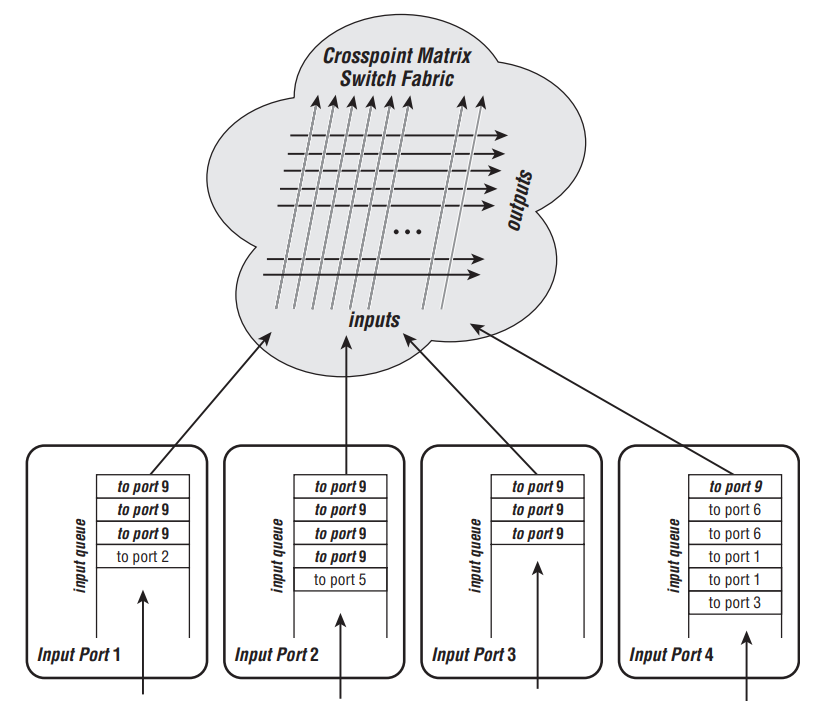
\includegraphics[width=0.9\textwidth]{HOL.png}
  \caption[Headh-of-line blocking]{Head-Of-Line Blocking (fonte: \cite{make})}
  \label{fig:airbus1}
\end{figure}



Na figura 3.3 encontra-se exemplificada uma situação em que as várias tramas do porto 4 não são transmitidas, ainda que os portos de destino das mesmas se encontrem livres. Técnicas que podem ser aplicadas para minimizar ou eliminar as limitações causadas por HOLB incluem equipar os portos com lógica capaz de requerer o envio de tramas que se encontrem em posições mais atrasadas nas filas ou incluir várias filas por porto. \par
Uma forma de contornar as limitações no débtito causados por HOLB é com recurso a OQs (\textit{Output Queue}) ao invés de IQs. Estas funcionam como filas de tramas com destino a um determinado porto. Desse modo, o HOLB desaparece porque a única situação em que uma trama não está a ser transmitida para o porto respetivo é se esse porto já estiver a receber uma outra trama. No entanto, a \textit{switch fabric} necessita de estar preparada para, no pior cenário, transmitir tramas de todos os portos de origem para um mesmo porto de destino, ou seja, o débito nas OQs tem que ser acelerado por um fator equivalente ao número de portos do switch.\par 
Uma opção alternativa é o recurso a VOQs (\textit{Virtual Output Queue}). Esta é uma variante das IQs, na qual, ao invés de haver uma fila em cada porto, há uma fila para cada par de portos origem-destino. De acordo com \cite{VOQ}, VOQs, em conjunto com um algoritmo do tipo \textit{round-robin} para atribuição de permissão de transmissão e recepção de tramas, alcança débitos à saída do switch muito próximos daqueles conseguidos via OQs, sem requerer que a \textit{switch fabric} seja capaz de transferir tramas para um porto com um débito mais elevado do que aquele com que o porto transmite as tramas para os cabos de \textit{Ethernet}. De acordo com \cite{math}, com recurso a uma aceleração por um fator de apenas dois, torna-se possível garantir o mesmo débito que com uma arquitectura com recurso a OQs. \par

 % file "Thesis_Implementation.tex"
\cleardoublepage

%\input{Thesis_new_file} % add new .tex files for new chapters
%\cleardoublepage

%\input{Thesis_new_file} % add new .tex files for new chapters
%\cleardoublepage

%\input{Thesis_new_file} % add new .tex files for new chapters
%\cleardoublepage

%%%%%%%%%%%%%%%%%%%%%%%%%%%%%%%%%%%%%%%%%%%%%%%%%%%%%%%%%%%%%%%%%%%%%%%%
%                                                                      %
%     File: Thesis_Results.tex                                         %
%     Tex Master: Thesis.tex                                           %
%                                                                      %
%     Author: Andre C. Marta                                           %
%     Last modified : 29 Jan 2021                                      %
%                                                                      %
%%%%%%%%%%%%%%%%%%%%%%%%%%%%%%%%%%%%%%%%%%%%%%%%%%%%%%%%%%%%%%%%%%%%%%%%

\chapter{Proposta de Arquitectura}
\label{chapter:results}

A arquitectura de um dispositivo deve ser cuidadosamente fundamentada num conjunto de metas que se pretendem assegurar, definindo as melhores estratégias para as cumprir o melhor que se possa com os recursos disponíveis. Neste trabalho decidiu-se que o mais importante seria procurar ao máximo assegurar a transmissão de todas as tramas que se apresentem ao dispositivo, tal como a correta execução do PTP. De modo que não ocorram situações em que o comutador tenha que descartar uma dada trama em detrimento de outras, é necessário que a arquitectura escolhida seja capaz de transmitir tramas com o mesmo débito com que as recebe. No entanto, devido ao estágio inicial em que se encontra o projeto no qual se insere este trabalho, ainda não há conhecimento das características das redes em que este dispositivo possa ser inserido. Assim, tentar-se-à maximizar o débito no dispositivo de acordo com o tempo disponível para a elaboração do mesmo. 


\section{\textit{Switch fabric}}


Como discutido no capítulo anterior, o débito num comutador é, essencialmente, limitado pela topologia escolhida para o módulo \textit{switch fabric}. Dessa forma, a escolha natural é a implementação de uma matriz \textit{crosspoint} em conjunto com VOQs. Um algoritmo responsável port corresponder os portos de transmissão com os portos de recepção foi encontrado em \cite{iSLIP}, denominando-se de iSLIP. De acordo com o  artigo, o algoritmo permite manter o débito na \textit{switch fabric} igual ao débito teórico máximo em circunstâncias de tráfego uniforme, com reduzidas limitações em situações de tráfego não uniforme. Além disso, o algoritmo garante que um porto não fica indefinidamente sem ser servido pela \textit{switch fabric}. A escolha do iSLIP deveu-se às referidas vantagens e também ao facto de ter uma implementação bastante simples, reduzindo o tempo necessário ao seu desenvolvimento, assim como o \textit{hardware} necessário.\par O iSLIP é um algoritmo de atribuição de correspondências em formato \textit{round-robin}. Cada porto que transmite tramas possui uma lista ordenada de prioridades de recepção por parte dos portos de destino. Além disso, possui também um codificador de prioridades, que a cada iteração determina qual o porto com prioridade mais elevada, de entre aqueles que dão permissão de envio. No momento de atualizar a lista de prioridades, todos os portos sobem uniformemente a sua prioridade, excetuando o porto no topo da lista de prioridades, que se torna o menos prioritário. Assim, resulta, que entre dois quaisquer portos num dado momento, aquele que tem maior prioridade é o que se encontra há mais tempo sem estar no topo da lista de prioridades. Da mesma forma, os portos de destino possuem igualmente uma lista da ordem de prioridades de envio de tramas por parte dos portos de origem. Além disso, tal como os portos de origem, estes possuem também um codificador de prioridades. O algoritmo funciona à base de iterações e a cada ronda do algoritmo é maximizada a correspondência (ou \textit{match}) entre os portos de origem e os portos de destino na quantidade de iterações definidas. Cada iteração está dividida em 3 fases: \textit{request}, \textit{grant} e \textit{accept}. Na fase de \textit{request}, cada porto de origem comunica a cada porto de destino se tem uma trama para lhe enviar. Na fase de \textit{grant}, cada porto de destino, tendo recebido a comunicação de quais os portos de origem que lhe querem enviar tramas, oferece uma permissão ao porto de origem que tiver a maior prioridade. Na fase de \textit{accept}, cada porto de origem decide transmitir ao porto de destino com maior prioridade de entre aqueles que lhe deram a sua permissão.\par A figura 4.1 ilustra um exemplo de funcionamento do algoritmo iSLIP.

\begin{figure}[!htb]
  \centering
  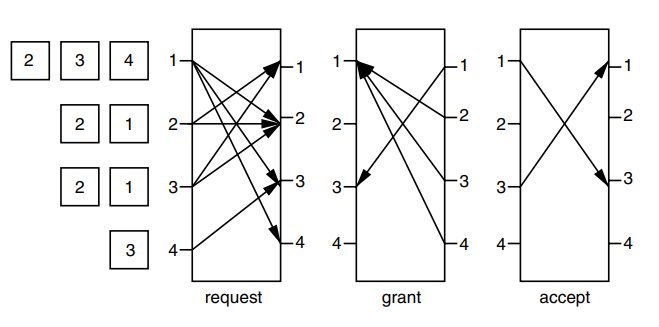
\includegraphics[width=1\textwidth]{imagem_islip.png}
  \caption[Iteração do iSLIP]{Iteração do iSLIP (fonte: \cite{math})}
  \label{fig:airbus1}
\end{figure}


Na fase de \textit{request}, o porto 1 requer o envio de tramas para os portos 2, 3, e 4; o porto 2 requer o envio para os portos 2 e 1; o porto 3 requer o envio para os portos 2 e 1; o porto 4 requer o envio para o porto 3. Na fase de \textit{grant}, o porto 1 oferece permissão de envio ao porto 3, enquanto os restantes portos oferecem permissão ao porto 1. Na fase de \textit{accept}, o porto 1, de entre as permissões que lhe são atribuídas decide transmitir para o porto 3, enquanto o porto 3 decide transmitir para o porto 1. Se o algoritmo acabar aqui, os portos 2 e 4 não têm opção de transmitir tramas, porque nenhum porto lhes deu essa permissão. Caso contrário, na iteração seguinte o algoritmo aumentará o \textit{match} correspondendo os portos de transmissão 2 e 4 relativamente aos portos de recepção 2 e 4.



Ao fim de uma iteração, nos portos de origem e destino que pertençam a uma correspondência, as listas de prioridades são atualizadas segundo a regra definida. Se o algoritmo estiver definido para uma iteração, a ronda acaba neste momento. Caso contrário, continua a tentar formar mais correspondências com os portos que ainda não pertençam a uma. Ao atualizar as listas de prioridade precisamente quando o respetivo porto fez parte de uma correspondência, a tendência a longo prazo será para haver dessincronização entre os elementos mais prioritários nas várias listas, reduzindo a ocorrência de exclusão de um porto no acesso à \textit{switch fabric}.


\section{Lógica de reencaminhamento}

No que diz respeito à tabela de endereços, dada a impossibilidade de utilizar uma memória CAM em FPGA, foi necessário pesquisar algoritmos de procura em tabelas implementados em \textit{hardware}. Numa análise exaustiva de alguns algoritmos, aplicados no contexto do protocolo HSR, foi encontrada uma solução \cite{HSR}. No documento são propostos três algoritmos para procurar e inserir elementos numa tabela.\par 
O primeiro algoritmo é denominado de "\textit{buffer} circular". Neste algoritmo, uma tabela é implementada juntamente com um ponteiro de escrita. De cada vez que é necessário escrever dados na tabela o ponteiro é incrementado. Excecionalmente, se o ponteiro se encontrar no fim da tabela, este volta para o início após uma escrita. Desta forma é garantido que as entradas da tabela que vão sendo retiradas são as mais antigas, permanecendo as mais recentes. A implementação desta solução é simples, no entanto, pode não ser a mais vantajosa se se desejar uma consulta da tabela consistentemente de curta duração. Em última análise, devido há falta de qualquer tipo de organização da tabela, será necessário percorrer toda a tabela para descobrir que um endereço não se encontra registado na mesma.\par 
Por forma a melhorar a eficiência temporal da procura na tabela, é analisado um segundo algoritmo com recurso a tabelas de dispersão. As tabelas de dispersão consistem em estruturas de dados que possuem alguma organização na distribuição da informação contida nos vários endereços de memória. Nestas tabelas, cada pedaço integral de informação que se pretende inserir ou procurar é mapeado através de uma função para um endereço de memória específico. Idealmente, as funções de dispersão devem ser totalmente aleatórias para reduzir a coincidência da função de dispersão de dois elementos diferentes, o que se denomina de colisão. No entanto, quando a quantidade de endereços de memória numa tabela não é várias ordens de grandeza maior que a quantidade de elementos possíveis de serem armazenados, as colisões tornam-se inevitáveis. Assim, torna-se necessário implementar técnicas que permitam manter presentes na tabela, em simultâneo, vários elementos que tenham sido mapeados para o mesmo endereço, e, posteriormente, aceder-lhes em momento de leitura. No estudo referido, foi implementada a técnica denominada \textit{Open Adressing}. Quando aplicada esta técnica, no momento de uma colisão, a procura pela informação pretendida continua para o endereço seguinte, segundo uma regra definida, até se encontrar os dados pretendidos ou se decida parar a procura. Por forma a não se dispensar demasiado tempo na procura, o autor definiu que a procura por um conjunto de dados estaria limitada a uma quantidade predefinida de endereços. Para finalizar o algoritmo, quando os dados não são encontrados nos endereços selecionados, os mesmos são inseridos no endereço cujo conteúdo foi mais antigamente acedido. Este algoritmo nunca procede a procuras tão lentas como o primeiro algoritmo poderá fazer, no entanto, a sua implementação é muito mais complexa devido ao mecanismo de rastreamento dos momentos de leitura das várias posições de memória.\par 
Por último, é proposto um algoritmo com a pretensão de ter uma eficiência semelhante ao segundo algoritmo, mas com uma complexidade de implementação semelhante ao primeiro algoritmo. Para isso, a tabela de endereços é divida num conjunto de \textit{buffers} circulares de reduzida dimensão, onde cada \textit{buffer} possui um ponteiro de escrita e um ponteiro de leitura. Tal como no segundo algoritmo, é aplicada uma função de dispersão. No entanto, esta mapeia os dados a procurar a um dos vários \textit{buffers} ao invés de a um endereçamento de memória. Após o mapeamento, o ponteiro de leitura é sucessivamente incrementado até que seja encontrado o que se procura ou se tenha percorrido a totalidade do \textit{buffer}. Quando não encontrados, os dados são guardados no endereço para o qual aponta o ponteiro de escrita, sendo este seguidamente incrementado. Quando a eficiência do algoritmo é medida como a probabilidade de serem encontrados na tabela os dados procurados, este algoritmo será teoricamente inferior ao anterior. A razão para isso prende-se com a escolha do endereço de memória a atualizar em caso de insucesso na procura. No segundo algoritmo, o endereço atualizado é aquele cujos dados permanecem hà mais tempo sem serem acedidos, face ao último endereço a ser escrito, que é a solução usada no terceiro algoritmo. 
\par Uma simulação em redes HSR de variada dimensão foi elaborada no estudo referido, onde foi validado o desempenho equiparável das duas variantes de tabela de dispersão. Assim, devido à maior simplicidade de implementação da tabela com recurso a um conjunto de \textit{buffers} circulares será essa a solução escolhida para operar como tabela de endereços.


 % file "Thesis_Results.tex"
\cleardoublepage

\chapter{Implementação}

Após a definição das funcionalidades a instalar e da arquitectura de suporte, inicia-se o processo de desenvolvimento do comutador. Para isso procede-se a uma descrição em Verilog do design escolhido. Verilog é uma linguagem usada para descrever um bloco de \textit{hardware} no requerido fluxo de dados entre os vários registos presentes no mesmo. A esse tipo de descrição denomina-se \textit{Register Transfer Logic} (RTL). No design global do comutador foram incluídos dois modelos de RTL muito versáteis e comuns. São eles:

\begin{itemize}
  \item \textit{Finite State Machines} (FSM) -\quad Máquinas de estados são modelos abstratos de computação que dividem o funcionamento de um módulo em diferentes operações consoante o estado em que se encontram. As máquinas de estados definem não só os vários estados como as transições entre os mesmos, que podem depender do estado atual, dos vários sinais que são dados à máquina de estados por outros módulos, ou de ambos. São bastante utilizadas devido à simplicidade de descrição e aos baixos recursos requeridos na sua implementação.
   \item \textit{First-In-First-Out} (FIFO) -\quad FIFOs consistem num bloco de memória na qual os dados são lidos na mesma ordem da sua escrita. Normalmente são implementadas com recurso a dois ponteiros. Um ponteiro com a posição do endereço de memória onde será feita a escrita seguinte, e um ponteiro com a posição de memória onde deve ser feita a seguinte leitura. No momento de uma escrita ou leitura os dois ponteiros são incrementados para garantir a coordenação referida da ordem da escrita e leitura na memória. 
   \iffalse
    \item \textit{Dual-Port-RAM} (DPRAM) -\quad Memória RAM que, contrariamente às convencionais, permitem a escrita e leitura simultânea na mesma. No dispositivo desenvolvido é o caso das filas previamente descritas.
    \fi
\end{itemize}

\section{Interfaces}

Para proceder à troca de informação entre nós de uma rede de \textit{Ethernet} e os canais de comunicação, é necessário que se use uma interface reconhecida por ambos os elementos. Devido à existência das várias iterações da \textit{Ethernet} disponíveis hoje em dia definiram-se várias interfaces diferentes, usualmente indicadas para canais de um débito pré-especificado. O comutador desenvolvido nesta dissertação deverá ser incluído numa rede a operar com débitos de canal de 1000 Mbit/s. Para esses, a interface usada é, tipicamente, a \textit{Gigabit media-independente interface} (GMII). Nesta, a recepção e transmissão ocorre segundo uma frequência de 125 Mhz, onde são recebidos pelo nó 8 bits no flanco ascende do relógio associado à recepção, e transmitidos 8 bits no flanco ascendente do relógio associado à transmissão.
Nas tabelas 5.1 e 5.2 estão identificados e descritos, respetivamente, os sinais de recepção e transmissão da interface GMII.\par Como se pode observar na tabela 5.2, a interface GMII inclui dois relógios associados à transmissão. Um deles, o GTXCLK é usado quando se pretende transmitir dados com o débitos de 1000 Mbit/s, ao passo que o TXCLK é usado quando o débito pretendido é de 10 Mbit/s ou 100 Mbit/s. No comutador desenvolvido, havendo apenas ao momento a indicação do requerimento de suportar o débito de 1000 Mbit/s, somente se gera o relógio GTXCLK.


\begin{table}[h]
\begin{center}
\begin{tabular}{|l|l|}

    \hline
    Sinal &  Descrição  \\
    \hline
    RXCLK &  Pulso de relógio recebido  \\
    \hline
    RXD[7:0] & Dados recebidos \\
    \hline
    RXDV & Indica que os dados recebidos são válidos \\
    \hline
    RXER & Indica que os dados recebidos contêm erros \\
    \hline
    
\end{tabular}
\end{center}
\caption{Sinais de recepção da interface GMII}\label{Sinais de recepção do GMII}
\end{table} 

\begin{table}[h]
\begin{center}
\begin{tabular}{|l|l|}

    \hline
    Sinal &  Descrição  \\
    \hline
    GTXCLK &  Pulso de relógio de 1000 Mbit/s transmitido  \\
    \hline
    TXCLK &  Pulso de relógio de 10 ou 100 Mbit/s transmitido  \\
    \hline
    TXD[7:0] & Dados transmitidos \\
    \hline
    TXEN & Indica que os dados transmitidos são válidos \\
    \hline
    RXER & Indica que os dados transmitidos contêm erros \\
    \hline
    
\end{tabular}
\end{center}
\caption{Sinais de transmissão da interface GMII}\label{Sinais de transmissão do GMII}
\end{table}


\section{Modelo comportamental}

Nas secções seguintes será explicado detalhadamente de um posto de vista funcional o esquema interno do comutador desenvolvido com os seus vários módulos, o processamento interno de cada um, e os vários bits de informação que são trocados entre si. \par
O processo que decorre entre o início da recepção do preâmbulo de uma trama e a transmissão do término do FCS da mesma num porto diferente pode ser dividida, do ponto de vista dos módulos envolvidos, em 3 fases. Uma primeira fase na qual é procedida à recepção da trama, a criação de meta-dados da mesma fundamentais nas fases seguintes, e ao registo da trama e dos respetivos meta-dados nos vários blocos de memória presentes no comutador. Numa segunda fase, os módulos centrais do comutador, tais como a \textit{Switch Fabric}, procedem à lógica necessária para encaminhar as tramas dos blocos de memória onde se encontram para os portos de destino. Numa terceira fase é procedida a manipulações finais à trama que possam ser necessárias.   


\subsection{Recepção de uma trama}

Na figura 6.1 podem ser observados os vários módulos que participam no processo de recepção de uma trama num porto. Os módulos PTP \textit{Common Core} e \textit{Forward Logic} representados na imagem consistem em módulos centrais do comutador que comunicam com módulos presentes na fase de recepção de uma trama em todos os portos. Contrariamente, os restantes módulos observados são contidos no processo de recepção de um único porto, de forma que se replicam por todos os portos presentes no comutador. Alguns dos módulos possuem alguma complexidade, podendo conter submódulos. O funcionamento detalhado de cada um e alguns esquemas internos serão dados de seguida.  

\begin{figure}[H]
  \centering
  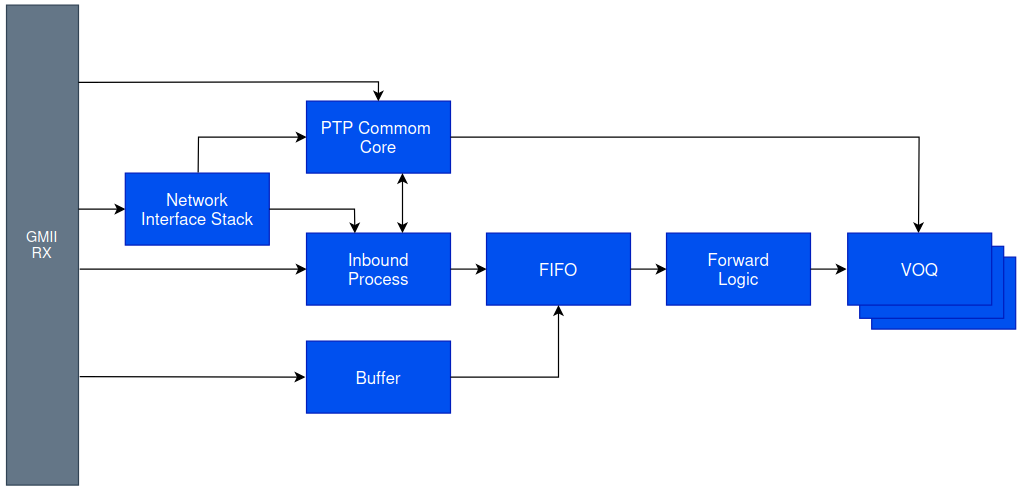
\includegraphics[width=1\textwidth]{FrameInbound.png}
  \caption[Processo de recepção de uma trama]{Processo de recepção de uma trama}
  \label{fig:airbus1}
\end{figure} 


\subsubsection{\textit{Inbound Process}}

O módulo \textit{Inbound Process} é o responsável por recolher um conjunto de meta-dados referentes ás tramas recebidas e por validar as mesmas para reencaminhamento. Para gerenciar a atividade do mesmo, este inclui uma máquina de estados. A máquina de estados é inicializada num estado de espera que remete a lógica de processamento de tramas do módulo para inatividade. Aquando da ativação do sinal RXDV avança-se sucessivamente para dois estados indicadores da recepção dos endereços MAC de destino e de origem da trama. Esses endereços são enviados para o módulo \textit{Forward Logic} onde serão usados no preenchimento e recolha de dados da tabela de endereços. Seguidamente, é identificado o \textit{EtherType} da trama. O valor do mesmo só é relevante se o mesmo for o \textit{EtherType} do PTP, o que é sinalizado ao módulo PTP \textit{Common Core}. Ainda que em certas normas como a IEEE 802.3 o campo que vem em seguimento ao campo do endereço MAC de origem possa comunicar o cumprimento do campo de dados da trama, o comutador recorre ao sinal \textit{RXDV} para delimitar a mesma. O último estado é aquele onde o módulo se encontra enquanto são recebidos o campo de dados e o FCS da trama, antes de voltar ao estado de espera. Há ainda um outro estado pelo qual o módulo pode passar caso seja identifica a presença da etiqueta de VLAN e de onde se recolhe a informação da prioridade da trama.   \par 
Se em qualquer momento durante o processamento da trama houver indicação de congestionamento da FIFO, indicação de congestionamento do \textit{Buffer}, indicação de que a trama é portadora de uma mensagem do PTP não passível de reencaminhamento, ou identificação de um erro, a trama não é aprovada para reencaminhamento e a decisão é comunicada ao \textit{Buffer}. Os erros possíveis de serem identificados pelo \textit{Inbound Process} são:

\begin{enumerate}
\item Erro no preâmbulo - \quad Erro identificado quando o preâmbulo e SFD não têm os valores esperados. 
\item Erro indicado pelo PHY - \quad Erro identificado quando o sinal RXER do respetivo porto se encontra com o valor lógico 1 aquando da recepção de um octeto da trama.
\item Erro no tamanho da trama -\quad Erro que ocorre quando o tamanho da trama é inferior ou superior aos limites definidos para as tramas do tipo \textit{Ethernet} II. Por forma a identificar este tipo de erro, o módulo inicia uma contagem aquando do início da recepção do campo de dados. Se suceder que a contagem ultrapasse o valor 1504 sem haver alteração do sinal RXDV, assume-se que a trama excedeu os 1500 octetos de dados permitidos somados aos 4 octetos do FCS. Da mesma forma, uma trama é interpretada como sendo demasiado pequena quando o valor do RXDV se torna 0 antes de a contagem chegar a 54, representativo dos 50 octetos do campo de dados mínimo somados aos 4 octetos de FCS. Futuramente, se, como é expectável, o comutador vier a ser incluído numa rede executante dos protocolos HSR ou PRP, os referidos valores dos limiares aceitáveis para o tamanho deverão ser ajustados para acomodar campos específicos dos referidos protocolos.  
\item Erro no FCS -\quad Aquando da mudança do sinal RXDV para 0, caso não tenha sido detetado um dos erros previamente descritos, pode ainda ser identificado um erro se o FCS que vem no fim da trama não coincidir com o FCS que é calculado no módulo. Um módulo capaz de calcular CRCs é incluído em cada módulo \textit{Frame Process} do comutador para esse efeito. 
\end{enumerate}

\subsubsection{\textit{Buffer}}

Blocos de memória na fase de recepção de tramas de um porto, onde é guardada a informação das referidas tramas, desde o preâmbulo até ao FCS. A estratégia escolhida passou por guardar as tramas num conjunto de segmentos de tamanho igual e pré-definido. Os segmentos precisam de ter uma dimensão suficiente para registar toda a informação referida anteriormente. Por exemplo, para uma situação em que o campo de dados tem o tamanho máximo de 1500 octetos, somando 22 octetos dos restantes campos, se se assumir 4 segmentos por trama, cada segmento deve ter capacidade para registar o mínimo de 593 octetos. Um exemplo de como as tramas podem ser guardadas num \textit{Buffer} pode ser observado na figura 6.2. Neste, podem ser identificadas duas tramas, a trama A e a trama B. A trama A está guarda nos segmentos com índice 1, 7 e 8, enquanto que a trama B está guardada nos segmentos com os índices 2, 3, e 6. Os restantes segmentos do \textit{Buffer} podem conter partes de tramas já recebidas ou encontrarem-se livres.


\begin{figure}[H]
  \centering
  \includegraphics[width=0.2 \textwidth]{Segments2.png}
  \caption[Buffer descontíguo]{Buffer descontíguo}
  \label{fig:airbus1}
\end{figure} 



 
O registo de uma trama no \textit{Buffer} no segmento disponível de índice mínimo inicia-se assim que o sinal TXDV é recebido com o valor lógico 1, marcando o segmento como indisponível numa tabela para isso criada. Após o preenchimento da totalidade do segmento, a escrita é transferida imediatamente para o segmento disponível seguinte, e assim sucessivamente, até que o sinal TXDV volte para o valor lógico 0. No final, se for recebida a informação por parte do módulo \textit{Inbound Process} que a trama não foi aprovada para reencaminhamento, os segmentos são novamente marcados como livres na lista sem haver necessidade de remover o conteúdo do \textit{Buffer}. A quantidade de leituras que deve ser feitas de cada segmento será dependente de a trama ser enviada em modo \textit{unicast} ou \textit{multicast}, sendo essa informação disponibilizada posteriormente pelo módulo que gere as VOQ. 

\subsubsection{PTP \textit{Common Core}}

O módulo PTP \textit{Common Core} é onde são analisadas as mensagens do protocolo \textit{PTP} e geradas as respostas em concordância com o protocolo. Na figura 5.3 está ilustrada a estrutura simplificada do módulo. Por forma a possibilitar a recepção de tramas portadoras de mensagens do PTP em todos os portos do comutador em simultâneo existe uma estrutura destas dedicada a cada porto. 


\begin{figure}[H]
  \centering
  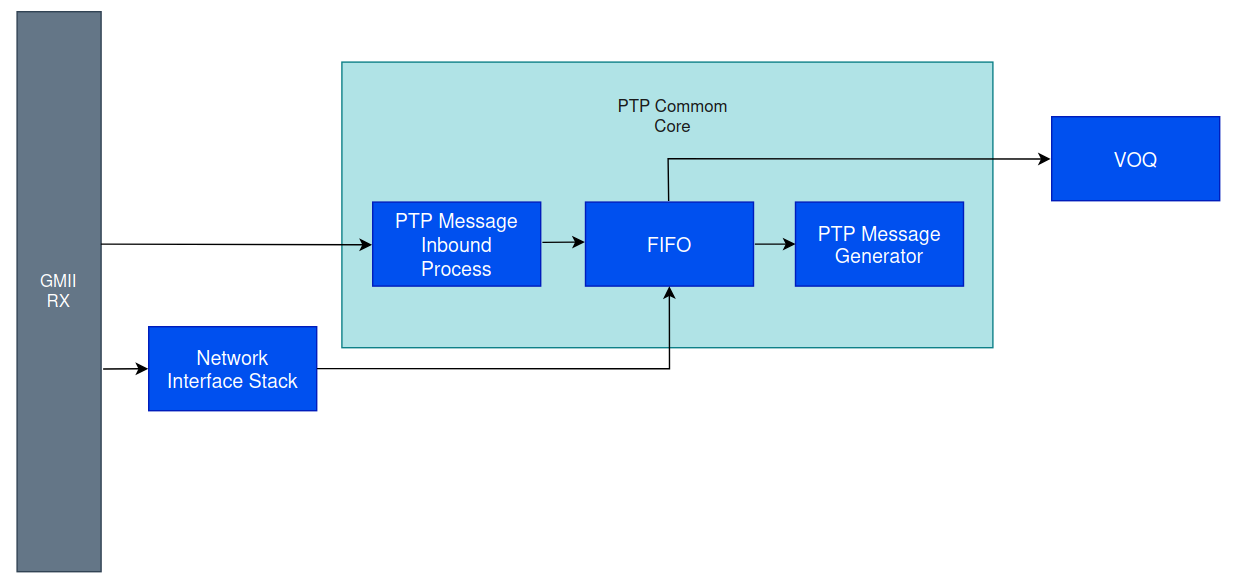
\includegraphics[width=1 \textwidth]{CommomCore.png}
  \caption[PTP Commom Core]{PTP Commom Core}
  \label{fig:airbus1}
\end{figure} 

O módulo PTP \textit{Message Inbound Processo} é onde são analisadas as mensagens do PTP recebidas e tomadas as decisões sobre como proceder. As quatro decisões possíveis, cujas circunstâncias causadoras foram explicadas no subcapítulo 2.4.1 são as seguintes:

\begin{enumerate}
    \item -\quad Permitir o reencaminhamento da trama sem requeres a alteração do \textit{correctionField}.
    \item -\quad Permitir o reencaminhamento da trama requerendo a alteração do \textit{correctionField}.
    \item -\quad Unicamente descartar a trama.
    \item -\quad Descartar a trama e iniciar o processo de resposta com uma trama portadora de uma mensagem \textit{PDelay\_Resp}.
\end{enumerate}

Quando é tomada a decisão de gerar uma mensagem \textit{PDelay\_Resp}, os campos \textit{sequenceId}, \textit{sourcePortIdentity}, \textit{correctionField}, e instante de recepção da mensagem \textit{PDelayReq} são capturados e colocados na FIFO presente no PTP \textit{Common Core}, onde aguardam até poderem ser inseridas na VOQ correspondente. Também na mesma FIFO são inseridas as indicações do requisito de transmissão das mensagens \textit{PDelay\_Req} nos momentos oportunos. 
 

\subsubsection{FIFO}
FIFOs onde são guardados os meta-dados referentes a uma trama. Os meta-dados consistem no tamanho da trama, o endereço MAC de destino e origem, a prioridade da mesma, um bit identificador de uma mensagem PTP da classe evento, o instante de recepção pelo comutador e os índices dos segmentos do \textit{Buffer} onde é guardada a trama. Um bit sinalizador do estado de FIFO vazia é fornecido ao módulo \textit{Frame Process} enquanto que outro sinalizador de FIFO cheia é fornecido ao módulo MAC \textit{Table Controller}. 


\subsubsection{\textit{Forward Logic}}

O módulo \textit{Forward Logic} é o responsável por proceder à gestão da tabela de endereços com recurso ao algoritmo explicado no capítulo 4. O módulo é único no comutador e recebe como sinais de entrada os bits indicadores de se as FIFO's previamente mencionadas se encontram ou não vazias. O módulo tem um estado de espera predefinido durante o qual aguarda que alguma fila deixe de estar vazia. Quando o bit de entrada de uma das vilas indica que esta não se encontra vazia, o módulo MAC \textit{Forward Logic} requer a leitura do elemento no topo da fila onde se encontram, entre outros dados, o endereço MAC de destino e origem da trama. Seguidamente, o módulo procede ao cálculo do CRC dos endereços MAC de destino e origem da trama que é usado como função de dispersão. Após o cálculo dos CRC's, é executada a procura dos endereços e possível atualização da tabela como explicado no capítulo 4. Para minimizar o tempo que uma trama se encontra no comutador, a procura do endereço de destino incluído na trama é efectuada antes da procura pelo endereço de origem. A conclusão do processo de procura do endereço de destino, juntamente com a informação do porto ou portos de destino da mesma, são imediatamente comunicados ao módulo responsável por atualizar as VOQs. 

\subsubsection{VOQ}

Filas de metadados referidas no capítulo 4. A quantidade de VOQs instaladas na fase de recepção de cada porto é dada pelo produto da quantidade de portos do comutador pela quantidade de prioridades de transmissão definidas. Os referidos metadados consistem nos índices dos vários segmentos do \textit{Buffer} onde se encontra guardada a trama, o instante de recepção da trama pelo porto, o tamanho da trama, e um código que indica se a trama contém uma mensagem do PTP.  A inserção é efectuada após a indicação do porto de destino da trama ou da transmissão em modo \textit{broadcast} por parte do módulo \textit{Forward Logic}. Quando a indicação é de proceder à transmissão para um único porto, os metadados são inseridos na VOQ correspondente ao porto destino e à prioridade da trama comunicada pelo módulo \textit{Inbound Process}. Alternativamente, quando a indicação é para reencaminhar a trama em modo \textit{broadcast}, os meta-dados são inseridos em todas as filas da respetiva prioridade, excluindo a fila que reencaminharia a trama de regresso ao porto por onde foi recebida.\par
 A inserção dos metadados referentes a tramas portadoras de mensagens \textit{PDelay\_Req} e \textit{PDelay\_Resp} ocorre quando solicitada pelo módulo PTP \textit{Common Core}, e é efectuada numa VOQ que represente o envio de uma trama de um porto para si mesmo. Para estas, os metadados consistem apenas no código respectivo Para reduzir o tempo que as tramas portadoras de mensagens do PTP permanecem no comutador, os seus metadados são sempre inseridos em filas de prioridade máxima.


\subsection{Reencaminhamento das tramas}

O processo de reencaminhamento das tramas é executado por dois módulos, \textit{Switch Fabric} e \textit{Switch Fabric Interface}. O módulo \textit{Switch Fabric} é exclusivamente responsável por receber os pedidos de transmissão de cada porto, selecionar os reencaminhamentos e providenciar os vários percursos que permitam a execução desses reencaminhamentos de tramas entre os portos. 
Por sua vez, o módulo \textit{Switch Fabric Interface} é responsável por proceder à comunicação entre os módulos da fase de recepção de tramas, os módulos que procedem às manipulações das tramas em fase de transmissão, e a \textit{Switch Fabric}. 
Seguidamente, segue uma descrição do funcionamento isolado de ambos.



\subsubsection{\textit{Switch Fabric}}

Na figura 5.4 é possível ser observada uma versão simples da estrutura interna do módulo \textit{Switch Fabric}.

\begin{figure}[H]
  \centering
  \includegraphics[width=0.3 \textwidth]{Fabric.png}
  \caption[\textit{Switch Fabric}]{\textit{Switch Fabric}}
  \label{fig:airbus1}
\end{figure} 

O seu submódulo principal é aquele denominado de iSLIP que executa o algoritmo homónimo descrito no capítulo 3. Por forma a maximizar sempre a correspondência entre portos a requerer o reencaminhamento de tramas, e os portos disponíveis para as receber, o módulo executa várias iterações do algoritmo até que não haja mais correspondências possíveis. \par Tal como muitos dos restantes módulos do comutador, este inclui uma máquina de estado para controlar a execução do algoritmo. Por defeito, a máquina de estados encontra-se num estado de espera, na qual o módulo iSLIP se encontra inativo. A transição para execução do algoritmo ocorre quando são transmitidos os pedidos de reencaminhamento de tramas por parte do módulo \textit{Switch Fabric Interface}. A execução do algoritmo decorre durante um único estado. Cada iteração decorre durante um ciclo de relógio desse estado, percorrendo os três estágios necessários: \textit{request}, \textit{grant} e \textit{accept}. No final da iteração, se for efectuada uma nova correspondência, o estado mantém-se, executando-se uma nova correspondência entre os portos não envolvidos nas correspondências já estabelecidas. Aquando da conclusão de uma iteração que não produza correspondências, a informação das correspondências estabelecidas é comunicada à \textit{Switch Fabric Interface}, e avança-se para um novo estado. Neste, decorre o envio do conteúdo das tramas dos portos de origem para os portos de destino através da matriz \textit{crosspoint} presente na \textit{Switch Fabric}. Esta consiste numa matriz de pontos de interseção que possuem dois conjuntos de entradas e saídas, e dois estados possíveis, representativos das duas formas possíveis de proceder a uma ligação bijetiva entre os referidos conjuntos. Uma representação da matriz pode ser observada na figura 5.5, juntamente com os respetivos pontos de interseção na figura 5.6.

\begin{figure}[H]
\centering
\begin{minipage}{.5\textwidth}
  \centering
  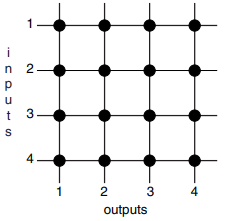
\includegraphics[width=.9\linewidth]{crossmatrix.png}
  \caption{Matriz \textit{crosspoint}}{(fonte: \cite{math})}
  \label{fig:test1}
\end{minipage}%
\begin{minipage}{.5\textwidth}
  \centering
  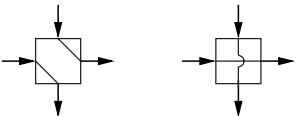
\includegraphics[width=.9\linewidth]{crosspoint.png}
  \caption{Ponto de interseção}{(fonte: \cite{math})}
  \label{fig:test2}
\end{minipage}
\end{figure}

A decisão sobre estados dos pontos de interseção que criam os caminhos entre os portos que possuem tramas a transmitir e os portos de destino correspondentes é efectuada pelo submódulo \textit{Matrix Control}. Para uma correta tomada de decisão a informação das correspondências é-lhe transmitida pelo módulo responsável por executar o iSLIP. 
Quando as tramas tiverem sido integralmente transmitidas, a conclusão do processo é comunicada pela \textit{Switch Fabric Interface}, regressando a \textit{Switch Fabric} a um estado de espera.  

\subsubsection{\textit{Switch Fabric Interface}}

O módulo \textit{Switch Fabric Interface} consiste num ponto de comunicação entre os módulos presentes na recepção e transmissão das tramas, e a \textit{Switch Fabric}, como pode ser observado na figura 5.7.

\begin{figure}[H]
  \centering
  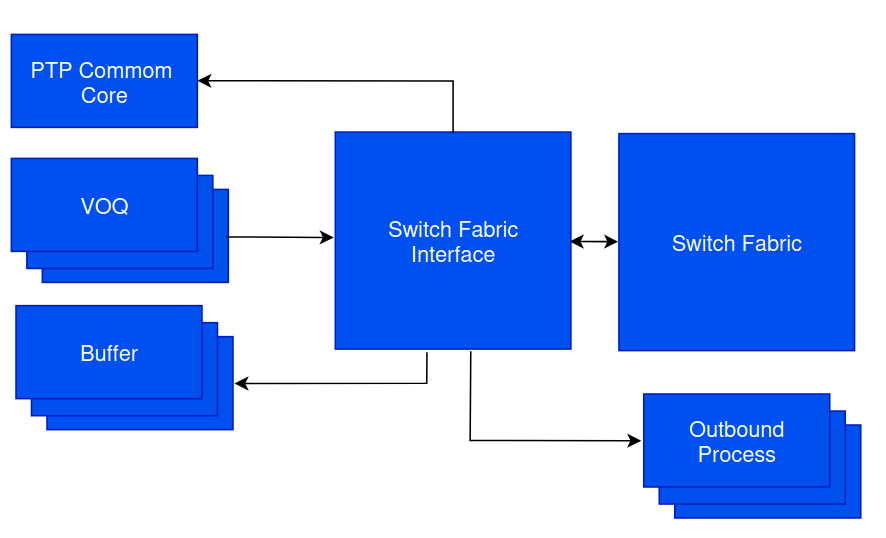
\includegraphics[width=1 \textwidth]{Interface_Fabric.png}
  \caption[\textit{Switch Fabric Interface}]{\textit{Switch Fabric Interface}}
  \label{fig:airbus1}
\end{figure} 


Esta é responsável por comunicar os pedidos de transmissão de tramas à \textit{Switch Fabric}, e, após providenciada a correspondência, requerer a leitura dos segmentos de memória dos \textit{Buffer}s onde estão guardadas as tramas. Ainda que haja troca de conteúdo das tramas entre a \textit{Switch Fabric} e outros módulos como o \textit{Buffer}, a responsabilidade da comunicação dos momentos adequados para a efectuar é da inteira responsabilidade da \textit{Switch Fabric Interface}.   \par
Para tirar o máximo de proveito das características da \textit{Switch Fabric} e do iSLIP, o momento em que é feito um novo pedido à \textit{Switch Fabric} situa-se imediatamente a seguir ao envio de todas as tramas por parte dos portos servidos previamente pela \textit{Switch Fabric}. Aí, para a criar o novo pedido de correspondências, a \textit{Switch Fabric Interface} apenas precisa de analisar o valor de um conjunto de sinais que indicam se as VOQs presentes no comutador estão, ou não, vazias.  


\subsection{Transmissão de uma trama}

Após a recepção na \textit{Switch Fabric Interface} da correspondência selecionada pela \textit{Switch Fabric} inicia-se o processo de envio das tramas para fora do comutador. Os módulos envolvidos na transmissão e as operações por si efectuadas variam consoante a trama seja gerada no comutador ou apenas reencaminhada. Seguidamente segue uma descrição das duas variantes do processo.

\subsubsection{Transmissão de tramas reencaminhadas}

Na figura 5.8 estão ilustrados os módulos que participam na transmissão de uma trama guardada num \textit{Buffer} do comutador após indicação do início do reencaminhamento por parte da \textit{Switch Fabric Interface}.

\begin{figure}[H]
  \centering
  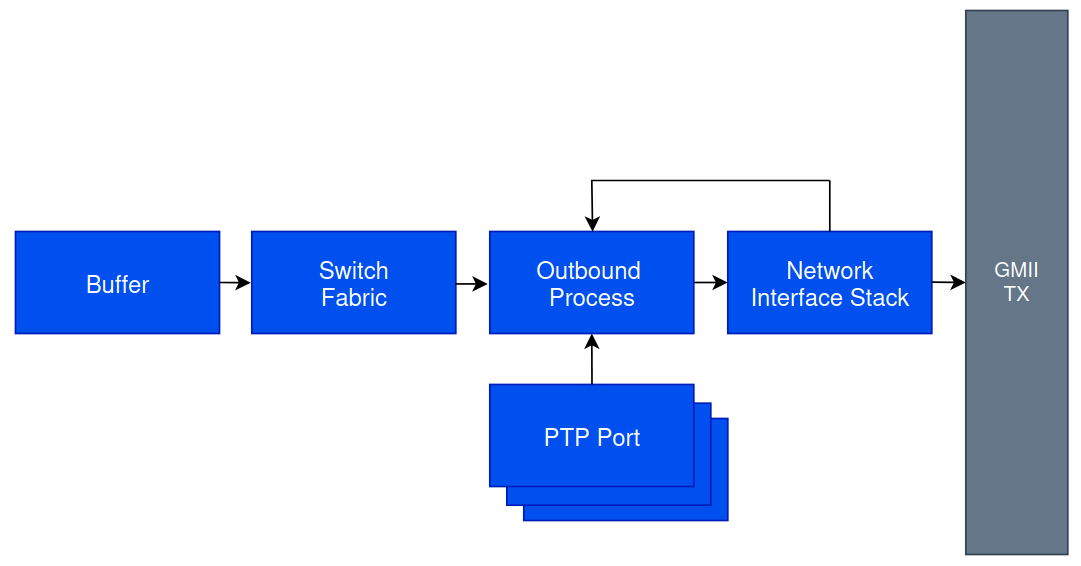
\includegraphics[width=1 \textwidth]{Outbound_Normal.png}
  \caption[Transmissão de tramas reencaminhadas]{Transmissão tramas reencaminhadas}
  \label{fig:airbus1}
\end{figure} 

Como explicado previamente, o conteúdo das tramas é guardada em segmentos dos \textit{Buffers} nos portos de recepção. Os ponteiros para as posições iniciais de cada segmentos são inseridos nas VOQs adequadas e recolhidos mais tarde pelo módulo \textit{Switch Fabric Interface} após a indicação por parte da \textit{Switch Fabric} de que pode começar a transmissão da referida trama. Assim que a \textit{Switch Fabric Interface} se encontre em posse dos ponteiros, esta indica aos \textit{Buffers} a leitura das tramas. \par 


Antes de sair do comutador, o fluxo de dados vindo dos \textit{Buffers} atravessa o módulo \textit{Outbound Process}. Este módulo, após receber a indicação do início da transmissão por parte da \textit{Switch Fabric Interface}, é responsável por fazer duas manipulações ao fluxo de dados recebido antes de o reencaminhar para a interface GMII. 

\begin{enumerate}
\item Alteração do \textit{correctionField} -\quad Para algumas mensagens do PTP já mencionadas anteriormente é necessário adicionar o tempo de residência e, em situações mais específicas, o \textit{meanLinkDelay} associado ao porto. O código identificador dessas mensagens é comunicado ao \textit{Outbound Process} pela \textit{Switch Fabric Interface}. Uma vez que, tanto as tramas de \textit{Ethernet} como as mensagens do PTP seguem um formato fixo, a posição do \textit{correctionField} na trama é constante para as tramas padronizadas da \textit{Ethernet}. Assim, para determinar o momento de manipulação do \textit{correctionField}, o módulo apenas precisa de iniciar uma contagem aquando do início da transmissão da trama que decorra até à posição previamente calculada do \textit{correctionField}. O instante de recepção da trama por um porto, de transmissão no porto adequado, e o \textit{meanLinkDelay}, são fornecidos ao módulo respetivamente pela \textit{Switch Fabric Interface}, \textit{Network Interface Stack} e PTP \textit{Port}.
\item Alteração do FCS -\quad Quando há alteração do \textit{correctionField} torna-se necessário calcular um novo FCS para a trama. Para isso, as tramas que são transmitidas por um porto são fornecidas a um módulo que calcula CRCs igual ao que se encontra presente no módulo \textit{Inbound Process}. No entanto, a responsabilidade de indicar o início e o fim da trama ao respetivo módulo e de inserir o código gerado na trama é da responsabilidade do \textit{Outbound Process}. A informação do tamanho da trama para isso necessária é-lhe fornecida pelo módulo \textit{Switch Fabric Interface}.
\end{enumerate}

\subsubsection{Transmissão de tramas \textit{PDelay\_Req} e \textit{PDelay\_Resp}}

Os módulos envolvidos na geração e consequente transmissão de uma trama portadora de uma mensagem \textit{PDelay\_Req} ou \textit{PDelay\_Resp} podem ser observados na figura 5.9.


\begin{figure}[H]
  \centering
  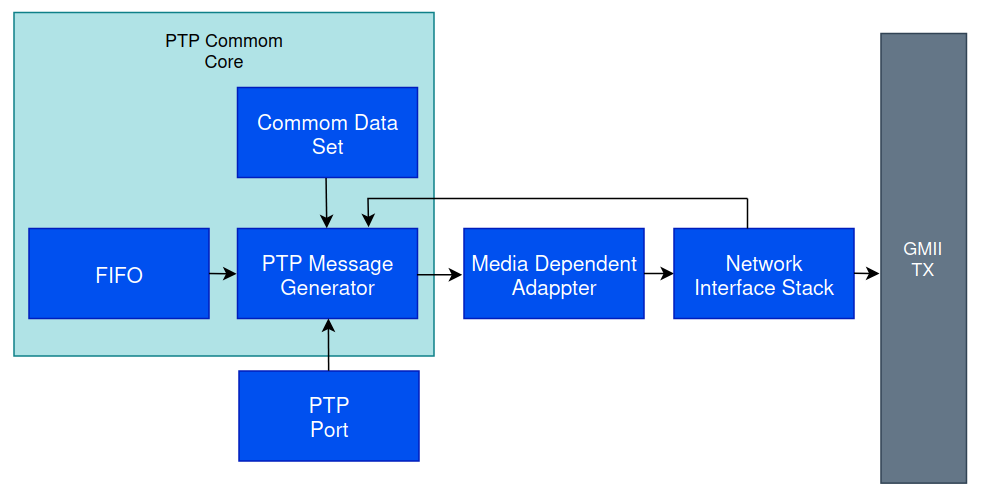
\includegraphics[width=1\textwidth]{PTP_Commom_Core.png}
  \caption[Transmissão de tramas \textit{PDelay\_Req} e \textit{PDelay\_Resp}]{Transmissão de tramas \textit{PDelay\_Req} e \textit{PDelay\_Resp}}
  \label{fig:airbus1}
\end{figure} 


Para facilitar a inclusão da capacidade de geração de tramas por iniciativa própria por parte do comutador, as tramas portadoras de mensagens \textit{PDelay\_Req} e \textit{PDelay\_Resp} requerem o acesso à \textit{Switch Fabric} em igualdade com as restantes tramas, ainda que não necessitem de reencaminhamento de um porto para outro. Desta forma, o início do envio destas tramas coincide com o início do envio de tramas reencaminhadas. Nesse instante, a \textit{Switch Fabric Interface}, com o conhecimento obtido através do código inserido na respetiva VOQ, informa o PTP \textit{Common Core} da autorização para a transmissão da respetiva trama portadora de uma mensagem \textit{PDelay\_Req} ou \textit{PDelay\_Resp}. A geração da trama começa, por indicação do PTP \textit{Common Core}, no módulo MD \textit{Adapter} presente no porto. Este é responsável por gerar todos os campos da trama à exceção do campo de dados com os seguintes conteúdos:


\begin{itemize}
  \item Preâmbulo -\quad 7 octetos com o valor 8xD5.
  \item SFD - \quad Um octeto com o valor 8x55.
  \item Endereço MAC de destino - \quad Como definido na norma, 01-80-C2-00-00-0E quando a trama contém uma mensagem utilizada no mecanismo P2P e 01-1B-19-00-00-00 para tramas que contenham uma das restantes mensagens.
  \item Endereço MAC de origem - \quad Endereço MAC do comutador que lhe é dado como parâmetro no código Verilog desenvolvido.
  \item \textit{EtherType} -\quad O \textit{EtherType} do PTP definido na norma, 16x88F7.
\end{itemize}


Após o preenchimento dos referidos campos, o MD \textit{Adapter} comunica ao PTP \textit{Common Core} o início da geração e transmissão do campo de dados.\par Para permitir a criação de mensagens relativas ao mecanismo P2P em simultâneo em todos os portos, o módulo PTP \textit{Common Core} possui um gerador dessas mensagens dedicado a cada porto. Esse gerador é responsável por preencher os vários campos do cabeçalho e corpo das mensagens com os vários valores das estruturas de dados presentes nos módulos PTP \textit{Port} e PTP \textit{Common Core}, e, no caso das mensagens \textit{PDelay\_Resp}, com recurso a alguns campos da mensagem \textit{PDelay\_Req} à qual se está a responder e do instante de transmissão da mensagem \textit{PDelay\_Resp}. Os dados provenientes da mensagem \textit{PDelay\_Req} são recolhidos da fila após a comunicação por parte da \textit{Switch Fabric Interface} da autorização para gerar a trama respetiva. O instante de transmissão da trama, necessário para preencher o \textit{correctionField} de uma mensagem do tipo \textit{PDelay\_Resp} é transmitido ao gerador pela \textit{Network Interface Stack} do respetivo porto.\par     
No fim da geração da mensagem do PTP o evento é comunicado ao \textit{MD Adapter}. Quando a mensagem a ser gerada é do tipo \textit{PDelay\_Resp}, este insere na trama o FCS calculado pelo módulo por isso responsável finalizando a criação da mesma.

\subsection{Cálculo do \textit{meanLinkDelay}}
O cálculo do \textit{meanLinkDelay} de um porto é da responsabilidade do respetivo PTP\textit{Port}. Nestes, cada um possui um contador que é incrementado todos os ciclos de relógio até decorrer 1 segundo que é o tempo de intervalo entre transmissões sucessivas de mensagens \textit{PDelay\_Req} definido na norma. Aí, o PTP \textit{port} requer o envio da mensagem ao PTP \textit{Commom Core} e fornece o \textit{sequenceId} respetivo ao mesmo. No momento em que a mensagem começa a ser gerada, o instante de transmissão da mesma, fornecido pelo \textit{Nerwork Interface Stack}, é registado pelo PTP \textit{Port}, assim como a sua associação ao \textit{sequenceId} da mensagem. O cálculo do \textit{meanLinkDelay} inicia-se no momento da recepção de uma mensagem \textit{PDelayResp} se o PTP \textit{Port} estiver a aguardar uma mensagem com o \textit{sequenceId} que vem na mesma e se o \textit{twoStepFlag} tiver o valor 0. Se o \textit{twoStepFlag} tiver o valor 1, o instante de recepção da mensagem, o seu \textit{correctionField} e o seu \textit{requestReceiptTimestamp} são registados em associação com o \textit{sequenceId} da mensagem. Aí, o cálculo acontece no momento da recepção da mensagem \textit{Pdelay\_Resp\_Follow\_Up} com o mesmo \textit{sequenceId}.\par
No instante em que o PTP \textit{Port} toma a decisão de atualizar o \textit{meanLinkDelay} as grandezas usadas são fornecidas a uma calculadora a isso dedicada. Dada a dimensão elevada dessas grandezas em quantidade de bits, para a calculadora ser sintetizável, as várias multiplicações e somas realizadas tiveram que ser subdivididas em operações com operandos de menor dimensão. 


\section{Opções de configuração}

Para tirar proveito da reconfigurabilidade das FPGA's, durante o desenvolvimento do comutador, o código Verilog do mesmo foi preferencialmente elaborado com recurso a parâmetros. Isso permite aumentar o conjunto de ambientes nos quais o comutador possa ser instalado, manipulando os parâmetros necessários. Os parâmetros existentes são os seguidamente descritos.

\begin{itemize}
  \item NUMBER\_PORTS  - \quad Define a quantidade de portos de Ethernet presentes no comutador. 
  \item SEGMENT\_SIZE  - \quad Define a quantidade de endereços de memória consecutivos num \textit{Buffer} que perfazem um segmento. 
  \item TOTAL\_SEGMENTS - \quad Define a quantidade de segmentos existentes no \textit{Buffer} associado a um porto.
  \item BIN\_SIZE - \quad Define o tamanho dos vários \textit{Buffers} circulares presentes na tabela de endereço.
  \item MAC\_TABLE\_SIZE - \quad Define a quantidade de \textit{Buffers} circulares presentes na tabela de endereços.
  \item VOQ\_FIFO\_SIZE -\quad Define a quantidade de elementos que podem ser armazenados em cada uma das várias VOQ's presentes no comutador. Precisa de ser um múltiplo de 2.
  \item PRIORITY\_QUEUE -\quad Define a quantidade de prioridades de diferentes com que as tramas podem ser diferenciadas pelo comutador. O valor deste parâmetro reflete-se na quantidade de VOQs que podem representar o envio de tramas entre cada par de portos.
  \item SLIP\_STAGES -\quad Define a quantidade de módulos consecutivos capazes de executar uma iteração do algoritmo iSLIP. Valores mais elevados neste parâmetro garantem uma execução mais rápida do iSLIP, pagando o custo de necessitar de mais recursos na implementação em FPGA.
  \item PTP - \quad Parâmetro que promove a instanciação de toda a lógica necessária para executar o protocolo PTP quando lhe é atribuido o valor 1. 
  \item COUNTERS - \quad Parâmetro que promove a instanciação de contadores de tramas úteis para calcular o desempenho do comutador e auxiliar em situações de depuração. Estes contadores permitem o registo da quantidade de tramas recebidas pelo comutador, a quantidade de tramas aprovadas para reencaminhamento, a quantidade de tramas rejeitadas por conterem erros, a quantidade de tramas descartadas por congestionamento de um \textit{Buffer}, a quantidade de tramas rejeitadas por congestionamento de uma VOQ, a quantidade de tramas transmitidas pelo comutador, e total de octetos contabilizados nas situações referidas. 
  \item ASYNC\_FIFO - \quad Quando com o valor 1, este parâmetro promove a instanciação de filas assíncronas, explicadas no capítulo seguinte.
\end{itemize}
  
Além dos referidos parâmetros, o comutador inclui ainda dois registos de configuração responsáveis por, separadamente, activar e desactivar o funcionamento como E2E \textit{Transparent clock} e P2P \textit{Transparent Clock}.  % file "DesenvolvimentoSwitch.tex"
\cleardoublepage

\chapter{Verificação do comutador}

\section{Princípios de verificação}

Após a descrição em Verilog do comutador é inevitável proceder a uma verificação exaustiva da correta funcionalidade do mesmo por forma a garantir o seu correto funcionamento em ambiente real, ou seja, no caso desta dissertação, em FPGA. Verificar o comutador estimulando-o trama a trama e observando as formas de onda dos sinais que servem como interface do mesmo pode dar uma primeira perspectiva do estado do mesmo, mas não é suficiente para garantir o seu correto funcionamento num ambiente real, na presença de tramas e erros de variados tipos. O \textit{testbench} deve ser capaz de cobrir o máximo do espaço de estímulos dos ambientes previsíveis de utilização do design desenvolvido, denominados de casos de teste, e proceder a uma validação autónoma da funcionalidade do mesmo nos vários ambientes. Para alcançar esta versatilidade, escalabilidade, e diminuir o tempo de desenvolvimento do mesmo, o \textit{testbench} deve ser dividido em várias componentes passíveis de reutilização em diferentes cenários e casos de teste. \par
O desenvolvimento de um \textit{testbench} em Verilog dificilmente não conduz unicamente à elaboração de testes diretos e a um formato monolítico do mesmo. Assim, é fulcral que o \textit{testbench} seja desenvolvido com uma linguagem possuidora de capacidades superiores de verificação. A linguagem usada na indústria e criada para esse propósito é o SystemVerilog \cite{SV}. Esta foi construida tendo Verilog como base e partilhando todas as suas capacidades de desenvolvimento, possuindo ainda capacidades adicionais ao nível de verificação, sendo por isso considerada, simultaneamente, uma linguagem de descrição de \textit{hardware} e uma linguagem de verificação de \textit{hardware}. As principais vantagens do SystemVerilog são a introdução de mecanismos de aleatoriedade, que permitem com maior facilidade abranger um vasto conjunto de estímulos diferentes no design, e o suporte para uma programação orientada por objectos que o dota da capacidade de ser usado para desenvolver \textit{testbenchs} com várias componentes passíveis de reutilização.\par
A estrutura típica de um \textit{testbench} desenvolvido em SystemVerilog foi, inicialmente, formulada no "\textit{Verification Methodoly Manual}" (VMM) \cite{VMM} e consolidada na metodologia UVM("\textit{Universal Verification Methodology}") \cite{UVM}, sem alterações a nível conceptual. Esta é hierárquica, dividindo o \textit{testbench} em várias camadas, onde as camadas superiores operam em níveis acrescidos de abstração. Os vários módulos presentes no \textit{testbench} trocam pacotes de informação representativos dos estímulos a injetar na DUT e das respostas capturadas denominados transações. O formato e conteúdo das transações pode ser variável consoante a posição na hierarquia das classes a comunicar, aumentando em detalhe quando na posse das classes de posição mais baixa na hierarquia.

\begin{itemize}
  \item \textit{DUT}  - \quad Abreviatura para "\textit{Design Under Test}", tipicamente usada para referir ao design que se está a verificar.  
  \item \textit{Environment}  - \quad Classe onde são construidos as várias classes do \textit{testbench}, separando-as do teste. 
  \item \textit{Driver}  - \quad Classe que contém os métodos que traduzem a informação contida numa transação para os vetores de bit's representativos da transação que são introduzidos nas interfaces correspondes da DUT.
  \item \textit{Monitor} -\quad Classe responsável por analisar os sinais à saida do DUT e comunicar os resultados à \textit{Scoreboard} para análise.
  \item \textit{Agent} -\quad Classe que recebe as transações originárias do \textit{Generator} e invoca os métodos das \textit{Driver}'s adequadas para produzirem a estimulação da DUT com as respetivas transações. Mais ainda, tipicamente, também é responsável por entregar as mesmas transações à \textit{Scoreboard}.
  \item \textit{Generator} -\quad Classe responsável por criar transações relevantes para a a verificação da DUT. Dependendo da complexidade do \textit{testbench} e da metodologia a ser seguida pode ser subdividido em dois módulos. Uma \textit{Sequence} responsável por criar uma transação singular e o \textit{Sequencer} responsável por requerer ao \textit{Sequence}, com as restrições necessárias, as transações indicadas para criar um cenário de teste. 
  \item \textit{Scoreboard} -\quad Classe que verifica se os sinais capturados à saída da DUT são os desejados para o teste a ser executado. Normalmente incluem o modelo de referência da DUT que simula o comportamento desejável na mesma. Os resultados capturados à saída da DUT são comparados com os previstos pelo modelo de referência para validar a correta funcionalidade da DUT.
  \item \textit{Test} -\quad Classe que inicializa o \textit{Environment} com as restrições e condições adequadas aos vários casos de teste. 
\end{itemize}

\section{\textit{Testbench} elaborado}

O primeiro passo na elaboração de um \textit{testbench} é definir os casos de teste e as métricas que se pretendem obter após a execução do \textit{testbench}. O comutador desenvolvido apenas tem a capacidade de interagir com as tramas portadoras de mensagens do PTP, sendo por isso irrelevante para a elaboração do \textit{testbench} qual o protocolo e conteúdo das restantes tramas.  Por sua vez, a interação com as tramas portadoras de mensagens do PTP depende do modo de operação do comutador. Assim, definiram-se dois casos de teste que consistem na implementação do comutador nos dois diferentes modos de execução do PTP. \par

O \textit{testbench} foi desenvolvido tendo por base transações representativas de tramas. Os valores destes campos são escolhidos de forma aleatório pelo \textit{generator}. Como as tramas são recebidas e enviadas em portos, para aumentar a escalabilidade e simplicidade de implementação do \textit{testbench} este foi construido com um \textit{generator}, \textit{agent}, \textit{driver} e \textit{monitor} por porto. A estratégia para verificar a correta funcionalidade do comutador passa por introduzir neste tramas unívoca e imediatamente identificáveis, registar o evento, e compara-las posteriormente com as tramas enviadas pelo comutador. A identificação das tramas é conseguida inserindo um código exclusivo da trama nos primeiro três octetos do campo de dados da mesma. Os identificadores necessários para cobrir todas as tramas criadas durante a execução do \textit{testbench} são gerados no \textit{environment} e entregues aos vários \textit{agents} previamente ao início dos testes. Um único tipo de transação representativo de tramas foi definido para ser trocado entre as várias classes do \textit{testbench}. As variáveis presentes na transação são os vários campos de dados do cabeçalho da trama, o comprimento do campo de dados e o referido identificador da trama. Para as tramas do PTP faz ainda parte da transação os campos de dados das mensagens do PTP. As tramas são criadas num \textit{generator} a pedido do \textit{agente} do respectivo porto. O \textit{generator} inclui métodos distintos para gerar transações representativas de tramas genéricas, tramas \textit{Sync}, tramas \textit{Follw\_Up}, tramas \textit{Delay\_Req}, tramas \textit{Delay\_Resp}, tramas \textit{PDelay\_Req}, tramas \textit{PDelay\_Resp} e tramas \textit{PDelay\_Resp\_Follow\_Up}. Após a recepção da transação no \textit{agent} este invoca os métodos da \textit{driver} que introduzem no comutador a trama representada pela transação. Tal como o \textit{generator}, este possui diferentes métodos consoante a transação represente uma trama genérica ou uma das várias tramas do PTP. A \textit{driver} inclui ainda a capacidade de inserir no comutador erros no PHY, CRC ou comprimento das tramas quando assim indicado pelo \textit{agent}. A periodicidade média do envio das tramas e da inserção de erros foi parametrizada no \textit{testbench} para permitir testar um conjunto mais diverso de cenários. As transações são também entregues à \textit{scoreboard} quando as tramas respetivas são introduzidas sem erros no comutador. \par 
Para capturar as tramas reencaminhadas pelo comutador, o \textit{testbench} inclui um \textit{monitor} por porto. Estes possuem um método responsável por capturar os vários campos de uma trama que é ativado no momento do flanco ascendente do sinal TXEN da interface GMII do respetivo porto. No final da recepção da trama, o \textit{monitor} cria uma transação que represente a respetiva trama e transmite-a para a \textit{scoreboard} juntamente com a informação da ocorrência ou ausência de erros. Os erros passíveis de identificação pelo \textit{monitor} são os três erros possíveis existentes em tramas de Ethernet, e a quebra do padrão definido para o campo de dados das tramas que não sejam do PTP. \par
A validação da correta execução do PTP e do reencaminhamento das tramas para os portos corretos é confirmada na \textit{scoreboard}. Para isso, a \textit{scoreboard} mantém uma lista por porto de transações que representem as tramas esperadas nesses portos. Essas listas são atualizadas no instante em que um \textit{agente} comunica à \textit{scoreboard} a introdução de uma trama no comutador.  Quando a trama não inclui uma mensagem do PTP, a \textit{scoreboard} apenas precisa analisar o endereço de destino da transação que representa a trama introduzida e adicionar a transação à lista de transações esperadas no respetivo porto. Para transações que representem tramas portadoras de mensagens do PTP, é computada uma transação esperada segundo as regras do protocolo explicadas em capítulos anteriores. Alguns campos da transação só são computados após a recepção da trama correspondente no \textit{monitor} e posterior comunicação à \textit{scoreboard}. O \textit{meanLinkDelay} dos vários portos do comutador, necessário para uma correta validação da execução do PTP port parte do comutador, é calculado de cada vez que uma trama \textit{Delay\_Resp}, \textit{PDelay\_Resp} e \textit{PDelay\_Resp\_Follow\_Up} é introduzida no comutador por uma \textit{driver}  \par
Para auxliar na decisão de término da execução do \textit{testbench} todos os \textit{monitors} incluem um contador que conta o tempo entre a última trama recebida e o instante de simulação presente. Quando esse valor ultrapassa um limiar previamente definido nos contadores de todos os monitores a execução do \textit{testbench} é terminada e os resultados obtidos são disponibilizados no terminal do Vivado.


\section{Latência e largura de banda obtidos}


Após a verificação permitir ter uma confiança elevada no funcionamento sem erros do comutados, o \textit{testbench} foi ampliado com a capacidade de calcular as latências e a largura de banda do comutador para diferentes tipos de tráfego. 

\begin{enumerate}
\item Tráfego ligeiro num único porto -\quad 
\item Tráfego exaustivo num único porto -\quad 
\item Tráfego ligeiro em todos os portos -\quad 
\item Tráfego exaustivo em todos os portos -\quad 
\end{enumerate}


Na tabela 6.1 podem ser observados os valores da latência e da largura de banda oferecidos pelo comutador para diferentes configurações dos parâmetros do mesmo e de volume de tráfego. Foram definidos quatro tipos de tráfego:

\begin{table}[h]
\begin{center}
\begin{tabular}{|l|l|}

    \hline
    &    \\
    \hline
     & \\
    \hline
     &   \\
    \hline
     &   \\
    \hline
     &  \\
    \hline
     &  \\
    \hline
    
\end{tabular}
\end{center}
\caption{Latência e largura de banda do comutador}\label{Latência e largura de banda do comuatdor}
\end{table}

 % file "Thesis_Implementation.tex"
\cleardoublepage

\chapter{Prototipagem em FPGA}

\section{Filas assíncronas}

A implementação de um circuito em ambiente físico requer o controlo de dificuldades que não são visíveis em simulações informáticas comportamentais do circuito. Devido à complexidade crescente dos circuitos uma situação que se vem manifestando de forma prevalente é a de transmitir informação entre registos que pertençam a diferentes domínios de relógio, onde um domínio consiste no conjunto de registos de um circuito que atualizam os seus estados no flanco de um relógio comum. Esta é normalmente conhecida por \textit{Clock Domain Crossing}(CDC). Na figura 7.1 é ilustrado o que pode suceder em CDC.  

\begin{figure}[H]
  \centering
  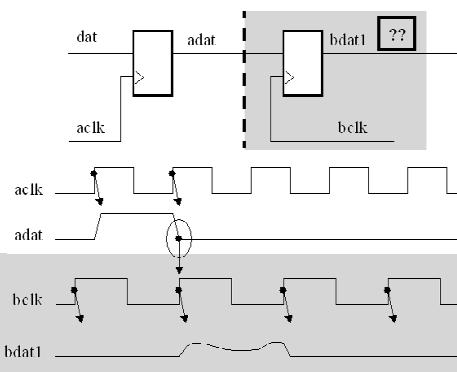
\includegraphics[width=0.55\textwidth]{CDC.png}
  \caption[\textit{Clock Domain Crossing} ]{\textit{Clock Domain Crossing} (fonte: \cite{CDC})}
  \label{fig:airbus1}
\end{figure}

Quando o sinal "adat" proveniente do domínio associado ao relógio "aclk" é capturado pelo registo no domínio associado a "bclk", o sinal à saída do registo pode passar por um período de metaestabilidade no qual flutua instavelmente entre bandas de valores proibidos. Entrando neste estado, não há garantias de que o sinal colapse para o valor lógico correto num período suficientemente reduzido de tempo que permite o normal funcionamento do circuito. O sinal metaestável pode propagar pelo circuito, ser capturado com diferentes valores em registos paralelos e consequentemente gerar uma disrupção no desejado funcionamento do circuito lógico. \par 
Em CDC, é muito improvável que possa ser evitado o aparecimento da metaestabilidade, no entanto, é possível contornar as suas consequências com recurso a técnicas para isso desenvolvidas. A mais básica e conhecida é a inserção de sincronizadores no circuito. Estes consistem numa sequência de registos associados ao domínio de relógio de destino, como se exemplifica na figura 7.2.

\begin{figure}[!htb]
  \centering
  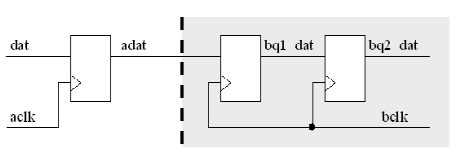
\includegraphics[width=0.65\textwidth]{synch.png}
  \caption[Sincronizador ]{Sincronizador (fonte: \cite{CDC})}
  \label{fig:airbus1}
\end{figure}


Recorrendo a um sincronizador suficientemente longo, é esperado que a metaestabilidade seja resolvida internamente ao mesmo, e que o correto valor do sinal seja, mais ou mais cedo, capturado à entrada do sincronizador. \par
Os sincronizadores servem, como descrito, quando o sinal a transitar entre domínios contém apenas um bit. No entanto, se se pretender transitar sinais com vários bits como, por exemplo, o sinal TXD da interface GMII, estes não são adequados. Ainda que previnam a metaestabilidade, não há garantia de que os vários bits sejam capturados pelo sincronizador num mesmo flanco de relógio. Para fazer a transição de domínios do referido sinal foram implementadas filas assíncronas. Uma ilustração do esquema interno de uma fila assíncrona pode ser observado na figura 7.3

\begin{figure}[h]
  \centering
  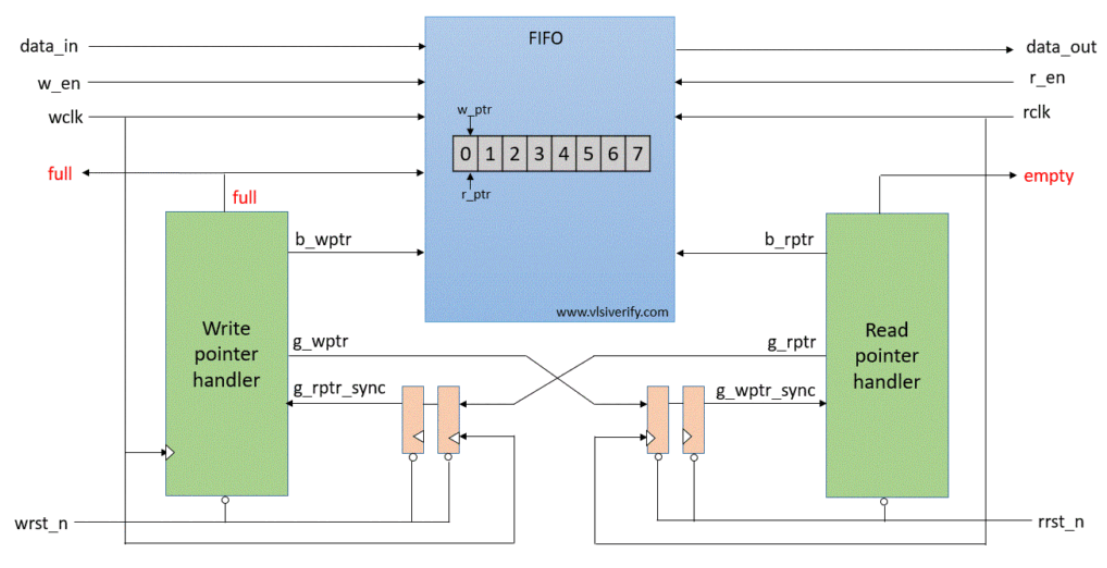
\includegraphics[width=0.9\textwidth]{AsyncFIFO.png}
  \caption[Fila assíncrona]{Fila assíncrona}
  \label{fig:airbus1}
\end{figure}


O esquema interno da fila assíncrona inclui um bloco de memória de profundidade variável, sincronizadores, e dois módulos responsáveis por gerenciar os ponteiros de escrita e leitura. O ponteiro de leitura dá a indicação da posição na fila de onde será efectuada a seguinte leitura, da mesma forma que o ponteiro de escrita dá a indicação da posição na fila da escrita seguinte. Após uma escrita o ponteiro de escrita é incrementado, tal como o ponteiro de leitura após uma leitura. A fila encontra-se cheia ou vazia quando os dois ponteiros indicam a mesma posição na fila. Para distinguir uma situação da outra um bit extra é adicionado ao ponteiro de escrita, duplicando a quantidade de posições que podem por si ser indicadas, de forma a trazer a indicação de que o referido ponteiro deu uma volta extra na fila em relação ao ponteiro de leitura. A comparação entre os dois ponteiros é efectuada pelos módulos denominados \textit{Write Pointer handler} e \textit{Read pointer handler}, que se encontram em domínios de relógio diferentes. Para transitar entre os dois domínios, todos os bits dos ponteiros passam por sincronizadores, como se observa na imagem. Como explicado previamente, tal não é possível se se tentar transitar dados, no entanto, para ponteiros isso é alcançável recorrendo a contadores de Gray. Estes contam segundo um código binário na qual entre dois valores consecutivos apenas há a mudança no valor lógico de um dos bits, ou seja, a distância de Hamming entre dois valores consecutivos é sempre de um. Na tabela 8.1 pode-se observar o código de Gray para os números entre 0 e 15, bem como o bit do código que se altera em cada transição. 

\begin{table}[H]
\begin{center} 
\begin{tabular}{|l|l|l|l|l|}

    \hline
    Decimal &  3 & 2 & 1 & 0 \\
    \hline
    0 & 0 & 0 & 0 & 0 \\
    \hline
    1 & 0 & 0 & 0 & \cellcolor{blue!25}1 \\
    \hline
    2 & 0 & 0 & \cellcolor{blue!25}1 & 1 \\
    \hline
    3 & 0 & 0 & 1 & \cellcolor{blue!25}0 \\
    \hline
    4 & 0 & \cellcolor{blue!25}1 & 1 & 0 \\
    \hline
    5 & 0 & 1 & 1 & \cellcolor{blue!25}1 \\
    \hline
    6 & 0 & 1 & \cellcolor{blue!25}0 & 1 \\
    \hline
    7 & 0 & 1 & 0 & \cellcolor{blue!25}0 \\
    \hline
    8 & \cellcolor{blue!25}1 & 1 & 0 & 0 \\
    \hline
    9 & 1 & 1 & 0 & \cellcolor{blue!25}1 \\
    \hline
    10 & 1 & 1 & \cellcolor{blue!25}1 & 1 \\
    \hline
    11 & 1 & 1 & 1 & \cellcolor{blue!25}0 \\
    \hline
    12 & 1 & \cellcolor{blue!25}0 & 1 & 0 \\
    \hline
    13 & 1 & 0 & 1 & \cellcolor{blue!25}1 \\
    \hline
    14 & 1 & 0 & \cellcolor{blue!25}0 & 1 \\
    \hline
    15 & 1 & 0 & 0 & \cellcolor{blue!25}0 \\
    \hline
    0 & \cellcolor{blue!25}0 & 0 & 0 & 0 \\
    \hline
    
\end{tabular}
\end{center}
\caption{Contador de Gray}\label{Contador de Gray}
\end{table}

\

Como nestes apenas há alteração no valor de um bit aquando do incremento do contador, o valor ponteiro pode demorar uma quantidade variável de ciclos a transitar para o outro domínio, mas nunca transitará com um valor inválido por dois bits diferentes serem capturados em momentos diferentes. As indicações de que a fila está cheia ou vaziam podem demorar uma quantidade indesejável de ciclos a atualizar, atrasar a escrita e leitura de dados na fila, no entanto, nunca se perderão dados. \par 
As filas assíncronas foram posicionadas imediatamente a seguir à recepção dos sinais da interface GMII, permitindo que toda a lógica necessária para receber, armazenar e retransmitir as tramas pudesse operar sobre um único domínio de relógio. A correta instalação das filas e consequente eliminação de possíveis problemas associados a CDC foi verificada com recurso ao \textit{software} \textit{Spyglas} desenvolvido pela \textit{Synopsys}.   



\section{Síntese}

O comutador foi desenvolvido prevendo a implementação futura do mesmo numa FPGA da Intel. Para comprovar a adequação da arquitectura do comutador para FPGA foi feita uma implementação do mesmo na placa de desenvolvimento de FPGA CYCLONE 10GX 10CX220YF780E5G. Esta é uma FPGA de gama média cujos recursos disponibilizados incluem 220000 \textit{lookup-tables} e 11740 kb de memória providenciados por 587 blocos de memória RAM de 20 kb. Sendo a FPGA da Intel, a implementação do comutador na mesma foi efectuada através do \textit{software} Quartus Prime. Na tabela 8.1 é possível observar os recursos necessários para a implementação do comutador na FPGA para diferentes quantidades de portos e em situações de inclusão ou ausência de filas assíncronas. \par   


Na tabela 7.2 podem ser observados recursos necessários para implementação em FPGA para diferentes quantidades de portos e com a possível adição de do suporte para o funcionamento como \textit{Transparent Clock}. Para todas as implementações foram definidos \textit{buffer}s compostos por 30 segmentos de 256 octetos, VOQs com 4 posições e duas prioridades diferentes, tabela de endereços com 128 \textit{buffer}'s circulares de 8 elementos, processador do iSLIP de um único andar, e sem inclusão de contadores e filas assíncronas. A síntese de versões do comutador com uma quantidade mais elevada de portos não foi possível devido à exaustão dos recursos da FPGA.

\begin{table}[h]
\begin{center}
\begin{tabular}{|l|l|}

    \hline
    &    \\
    \hline
     & \\
    \hline
     &   \\
    \hline
     &   \\
    \hline
     &  \\
    \hline
     &  \\
    \hline
    
\end{tabular}
\end{center}
\caption{Recursos da FPGA necessários para a síntese do comutador}\label{Recursos da FPGA necessários para a síntese do comutador}
\end{table} % file "ImplementacaoFPGA.tex"
\cleardoublepage

\chapter{Conclusões}

Nesta dissertação foi desenvolvido um comutador de Ethernet com suporte para a atuação como o elemento de rede denominado \textit{Transparent Clock} definido na norma do protocolo PTP. Numa primeira fase, estudou-se várias formas de implementar os elementos que constituem o comutador com foco em encontrar uma solução que permitisse optimizar o débito do mesmo com os recursos e tempo disponibilizados para o seu desenvolvimento. Seguidamente, foi também estudada robustamente a versão mais recente da norma que define o PTP. Após uma análise exaustiva foi decidido que o ponto de partida adequado seria a implementação do modo \textit{One-Way} dos mecanismos P2P e E2E. Após a decisão da arquitectura e das funcionalidades a implementar procedeu-se à elaboração de uma descrição em Verilog do circuito em formato RTL que implemente o comutador. Devido à complexidade da totalidade do modelo a descrever, esta tarefa requereu uma quantidade de tempo considerável daquele usado nesta dissertação. 

\section{Trabalho futuro}

Ainda que tenham sido finalizado com sucesso os objetivos pretendido com esta dissertação, o dispositivo desenvolvido continua longe de estar completo, e a aprovação em 2023 do PRR associado garante a continuidade do desenvolvimento aqui iniciado. A trajetória a tomar após a conclusão do trabalho realizado vai estar dependente das decisões tomadas pelos futuros responsáveis do mesmo, no entanto, considerando a indústria na qual se incluirá este dispositivo, deverá seguir uma das seguidamente mencionadas. \par

No que se refere ao PTP há muitas funcionalidades que não foram ainda implementadas. Além do funcionamento como \textit{Transparente Clock}, poderá ser do interesse dos detentores do comutador que este atue também como \textit{Ordinary Clock}. Para tal, será necessário executar o BMC e proceder ao cálculo dos tempos de propagação entre \textit{Master} e \textit{Slave} com recurso ao envio e manipulação das mensagens \textit{Sync}, \textit{Follow\_Up}, \textit{Delay\_Req} e \textit{Delay\_Resp}. A opção tomada de recorrer às estruturas de dados e módulos sugeridos na norma para implementação de uma instância prevê uma maior agilidade numa inclusão futura do suporte para funcionamento como \textit{Ordinary Clock}. Menos relevante, mas também possível de inclusão, é o suporte para o processamento das mensagens \textit{Signaling} e \textit{Management}, e das várias \textit{TLV}'s definidas na norma.
Os sistemas de automação de subestações são elementos fulcrais da indústria energética, por isso os seus serviços devem ser disponibilizados ininterruptamente. Tal pressupõe que as comunicações entre os dispositivos constituintes da mesma não devem ser interrompidas devido a falhas nos elementos responsáveis pelas comunicações. Para o evitar a rede de comunicações sobre Ethernet deve implementar protocolos preparados para providenciar caminhos de comunicação alternativos em caso de falha de um elemento de rede. Os dois mais conhecidos são o HSR e o PRP, e a implementação no comutador do suporte para um dos dois algoritmos será quase inevitável. \par 
Por último, é necessário cumprir com os requisitos de segurança comuns na indústria. Assim, deverá ser também implementado o MACsec(\textit{Media Access Control Security}) \cite{MACSec}. Este é um protocolo de segurança operado em redes LAN baseado no algoritmo Galois de encriptação recorrendo a chaves simétricas. O MACsec permite garantir a integridade e confidencialidade das tramas circulantes na rede. O MACsec não requer a adição de uma quantidade excessiva de recursos quando implementado em \textit{hardware}, e por essa razão a sua implementação no comutador será um passo natural. % file "TrabalhoFuturo.tex"
\cleardoublepage

% ----------------------------------------------------------------------
%  Bibliography
% ----------------------------------------------------------------------

% Add entry in the table of contents as chapter
\phantomsection
\addcontentsline{toc}{chapter}{\bibname}

% Include all references in .bib file, even non-cited ones...
%\nocite{*} % this should be used carefully because it is not correct!

% Produces the bibliography section when processed by BibTeX
%
% Bibliography style
% > entries ordered alphabetically
%\bibliographystyle{plain}
% > unsorted with entries appearing in the order in which the citations appear.
%\bibliographystyle{unsrt}
% > entries ordered alphabetically, with first names and names of journals and months abbreviated
%\bibliographystyle{abbrv}
% > entries ordered alphabetically, with reference markers based on authors' initials and publication year
%\bibliographystyle{alpha}
%
% Replacement bibliography styles provided by 'natbib' package
% (plainnat.bst, abbrvnat.bst, unsrtnat.bst )
% > entries ordered alphabetically
%\bibliographystyle{plainnat}
% > unsorted with entries appearing in the order in which the citations appear.
%\bibliographystyle{unsrtnat}
% > entries ordered alphabetically, with first names and names of journals and months abbreviated
%\bibliographystyle{abbrvnat} % <<<<< SELECT IF USING REFERENCES BY AUTHOR/YEAR
% > entries ordered alphabetically, with reference markers based on authors' initials and publication year
%\bibliographystyle{alpha}
%
% Custom bibliography style adapted from 'natbib' package
%   (based on http://tex.stackexchange.com/questions/5053/is-it-possible-to-get-unsrt-abbrv-bibliography)
%   (unsrtnat.bst + abbrvnat.bst -> abbrvunsrtnat.bst)
%   (original files copied from:
%   http://tug.ctan.org/macros/latex/contrib/natbib/abbrvnat.bst
%   http://tug.ctan.org/macros/latex/contrib/natbib/unsrtnat.bst
% > unsorted with entries appearing in the order in which the citations appear, with first names and names of journals and months abbreviated.
\bibliographystyle{abbrvunsrtnat} % <<<<< SELECT IF USING REFERENCES BY NUMBER (CITATION ORDER)

% External bibliography database file in the BibTeX format
\bibliography{Thesis_bib_DB} % file "Thesis_bib_DB.bib"

\cleardoublepage

% ----------------------------------------------------------------------
%  Appendix (optional)
%
%  CAUTION: 1) the main document (up to the conclusions) shall not exceed 80 pages
%           2) the document shall not exceed a total of 100 pages (per IST regulations)
% ----------------------------------------------------------------------


% add page number prefix according to apendix chapter (optional)
%\renewcommand{\thepage}{\thechapter.\arabic{page}}

% re-set arabic numbering (A.1,A.2,...) (optional, use only if chapter prefix is added)
%\setcounter{page}{1}



% re-set arabic numbering (B.1,B.2,...) (optional, use only if chapter prefix is added)
%\setcounter{page}{1}



% ----------------------------------------------------------------------
\end{document}
% ----------------------------------------------------------------------

${jrebel_args} "-Dprogram.name=JBossTools: Red Hat JBoss EAP 6.1+" -server -Xms2048m -Xmx2048m -XX:+UseParallelOldGC -XX:+AggressiveOpts -Dorg.jboss.resolver.warning=true -Djava.net.preferIPv4Stack=true -Dsun.rmi.dgc.client.gcInterval=3600000 -Dsun.rmi.dgc.server.gcInterval=3600000 -Djboss.modules.system.pkgs=org.jboss.byteman -Djava.awt.headless=true "-Dorg.jboss.boot.log.file=C:\Hercules\Apps\s10\jboss-eap-6.4\standalone\log\boot.log" "-Dlogging.configuration=file:C:\Hercules\Apps\s10\jboss-eap-6.4\standalone\configuration\logging.properties" "-Djboss.home.dir=C:\Hercules\Apps\s10\jboss-eap-6.4" -Dorg.jboss.logmanager.nocolor=true -Djboss.bind.address.management=localhost ${local_params}

​

-DOperationsTool.validateCatalogLoad=false -DOperationInterceptor.dontRegisterOperation=false -DOperationInterceptor.dontValidateDuplicated=false -DOperationInterceptor.dontValidateLimits=false -DOperationInterceptor.dontGoStoreAndForward=false -Dworkspace_loc=${workspace_loc} -Dceb.mock.mode=true -Djboss.as.management.blocking.timeout=900

http://localhost:8080/cdo/

https://jira.k8s2.grupocgd.com/browse/TCEM-3349 

https://wwwq.cgd.pt/Particulares/Pages/Particulares_v2.aspx

https://pce-bo.cqgrupocgd.com/bkoWeb/home.seam